\documentclass[12pt,twoside]{book}

% Idioma español
\usepackage[spanish,es-lcroman]{babel} % Características del idioma
\usepackage[utf8]{inputenc} % Acentos

% Espacio entre párrafos
\usepackage{parskip}

% Kerning y mejoras tipográficas
\usepackage{microtype}

\usepackage{xstring}
\usepackage{pgfkeys}

% Matemáticas: \text, \mathbf, \overset, \underset, equation*
\usepackage{mathtools}

% Listas numeradas
\usepackage{enumerate}

% Columnas
\usepackage{multicol}

\usepackage[a5paper]{geometry}

\usepackage{sectsty}

%\usepackage{ifthen}
\usepackage{tcolorbox}
\usepackage{xparse}
\usepackage{tikz}
\usetikzlibrary{matrix}

\ExplSyntaxOn
\DeclareExpandableDocumentCommand{\eval}{m}{\int_eval:n {#1}}
\ExplSyntaxOff

\newcounter{first}
\newcounter{doce}
\setcounter{first}{-1}

\newcommand{\md}[1]{
	\ifnum#1>\thedoce
		\ \eval{#1-\thedoce}
	\else\ifnum#1<0
		\ \eval{#1+\thedoce}
	\else #1
	\fi\fi
}
\newcommand{\row}[2]{%
	\foreach \i in {#1} {%
		\begingroup\edef\x{\endgroup
			\noexpand\gappto\noexpand\mymatrixcontent{ 
				{#2}\&
		}}\x
	}%
	\gappto\mymatrixcontent{\\}%
}
\newcommand{\mat}[1]{
	\let\mymatrixcontent\empty
	\setcounter{doce}{0}
	\setcounter{first}{-1}
	
	\foreach \n in {#1}{
		\ifnum\thefirst=-1
			\setcounter{first}{\n}
		\fi
		\stepcounter{doce}
	}
	
	\foreach \j in {#1}{
		\row{#1}{%
			\md{\eval{\i-\j+\thefirst}}
		}
	}

	\resizebox{\linewidth}{!}{
		\begin{tikzpicture}
		\matrix [ampersand replacement=\&, 
			matrix of math nodes, 
			row sep=0.2em, column sep=1em]
		{\mymatrixcontent};
		\end{tikzpicture}
	}
}
\usepackage{ddphonism}


\chapternumberfont{\Large}
\chaptertitlefont{\LARGE}

\newcommand{\full}{\resizebox{\linewidth}{!}}

\tikzstyle rotateArrow=[decoration={markings,mark=at position 0.9999 with {\arrow[scale=1,>=triangle 45]{>}}},postaction={decorate}]


% Colores
\usepackage{color}

% Código
\usepackage{listingsutf8}
\lstset{
	inputencoding=utf8,
	extendedchars=true,
	literate=%
	{á}{{\'a}}1
	{é}{{\'e}}1
	{í}{{\'i}}1
	{ó}{{\'o}}1
	{ú}{{\'u}}1
	{Á}{{\'A}}1
	{É}{{\'E}}1
	{Í}{{\'I}}1
	{Ó}{{\'O}}1
	{Ú}{{\'U}}1
	{ñ}{{\~n}}1
	{Ñ}{{\~N}}1
	{¿}{{>}}1
	{¡}{{<}}1
	{―}{{---}}1
}

% PDFs
\usepackage{pdfpages}

% Letras raras de matemáticas
\usepackage{upgreek} % \uptheta
\usepackage{amssymb} % \mathbb

% Tachar
\usepackage{soul}

% QED
\usepackage{amsthm}

% QR
\usepackage{qrcode}

% Notas musicales
\usepackage{wasysym}

% Más columnas en matrix
\setcounter{MaxMatrixCols}{30}

% Imágenes
\usepackage{graphicx}
\usepackage{wrapfig}
\usepackage{caption}
\graphicspath{{Fotos/}}

% Headers
%\usepackage{fancyhdr}
%\fancyhead{}
%\fancyhead[LE,RO]{\MakeUppercase{\chaptername\ \thechapter}}
% \setlength{\headheight}{15.71667pt}

% Apéndices
\usepackage[titletoc]{appendix}
\renewcommand{\appendixname}{Anexo}
\renewcommand{\appendixtocname}{ANEXOS}
\renewcommand{\appendixpagename}{Anexos}

% Dibujos TIKZ
\usepackage{tikz}

\newcommand*\cancel[2][thin]{\tikz[baseline] \node [strike out,draw,anchor=text,inner sep=0pt,text=black,#1]{#2};}  

% Clear double page limpio
\makeatletter
\def\cleardoublepage{\clearpage\if@twoside \ifodd\c@page\else
	\hbox{}
	\vspace*{\fill}
	\vspace{\fill}
	\thispagestyle{empty}
	\newpage
	\if@twocolumn\hbox{}\newpage\fi\fi\fi}
\makeatother

\newenvironment{changemargin}[2]{%
	\begin{list}{}{%
			\setlength{\topsep}{0pt}%
			\setlength{\leftmargin}{#1}%
			\setlength{\rightmargin}{#2}%
			\setlength{\listparindent}{\parindent}%
			\setlength{\itemindent}{\parindent}%
			\setlength{\parsep}{\parskip}%
		}%
		\item[]}{\end{list}}
	
\usepackage[hidelinks]{hyperref}
%\includeonly{02.Dodecafonismo, Portada, Introduccion, 08.Filosofia, 09.Escalas, 10.Musescore, Anexos, Bibliografia}

\begin{document}
	\small
	\pagestyle{plain}
	\thispagestyle{empty}
	
    \pagestyle{plain}
\thispagestyle{empty}

	\begin{center}
			\vspace*{\bigskipamount}
            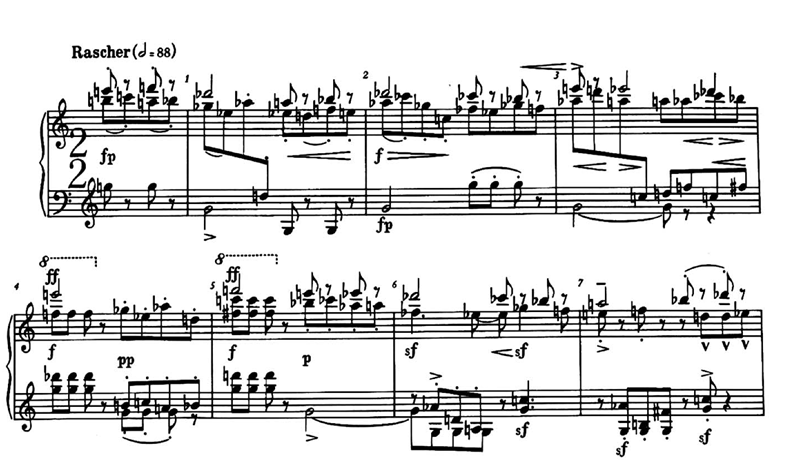
\includegraphics[width=\textwidth]{0.png}
            
			\vfill
			{\LARGE LA ESTRUCTURA MATEMÁTICA\\DEL SERIALISMO MUSICAL\par}
		
			\bigskip\bigskip\bigskip
			\large{Celia Rubio Madrigal\par}
            
	\end{center}

\newpage$\ $
\thispagestyle{empty}
\newpage
    
	\pagenumbering{Roman}
    \pagestyle{plain}
\thispagestyle{empty}

	\vspace*{\bigskipamount}
	\begin{flushright}
		\textit{Dedicado a mis dos \\
			grandes pasiones: \\
			las matemáticas \\
			y la música.} \\
		
		\vfill
		It has been observed that mathematics is the\\
		most abstract of the sciences, music\\
		the most abstract of the arts.\\
		\bigskip
		 --- David Wright \cite{wright}
	\end{flushright}
	
	\chapter*{Agradecimientos}
	
		Me gustaría dar las gracias a todos.
	
	
	\pagenumbering{Roman}
	\chapter*{INTRODUCCIÓN AL TEXTO}
		Todas las estructuras musicales están basadas en estructuras matemáticas. Los elementos musicales de los que están compuestas las obras, como las notas, las dinámicas o los timbres, están agrupados en conjuntos, y, como tales, cumplen ciertas propiedades al relacionarse consigo mismos o con otros conjuntos.
		
		A lo largo de la historia, los compositores han ido descubriendo e inventando estas propiedades musicales en las piezas que componían; por ejemplo, desde consonancias y disonancias entre notas, hasta la jerarquía según el pulso en el que la nota se encuentra. Las matemáticas son capaces de describir las propiedades de estos elementos musicales como para cualquier otro conjunto matemático.
		
		Por ejemplo, las músicas serialistas se basan en la continua reiteración de secuencias de elementos musicales. Es decir, un compositor serialista tomará una secuencia ordenada de notas, dinámicas o timbres y la usará como único bloque constructivo de su obra. Puede, además, serializar más de un conjunto de elementos musicales, o incluso pretender serializar el máximo número de conjuntos -- lo que a mediados del siglo XX se llamaría serialismo integral. Estas músicas se pueden describir matemáticamente por medio de permutaciones y grupos.
		
		Son en estas estructuras en las que se centrará el presente texto, y más específicamente en el dodecafonismo, el primer sistema compositivo serialista. Se explicarán los fundamentos matemáticos que lo posibilitan, las razones históricas por las que surgió y los postulados que lo definieron, proponiendo ejemplos analizados. Además, se investigará sobre el valor artístico del serialismo mediante el uso de escalas no cromáticas en busca de consonancia.
        % TODO
        
    
    \renewcommand*\contentsname{\begin{LARGE}\textbf{Índice general}\end{LARGE}\vspace{-\bigskipamount}}
	\begin{changemargin}{-0.5cm}{-0.5cm}
		\tableofcontents
	\end{changemargin}
	\newpage
	$\ $
	\thispagestyle{empty}
	\newpage
	$\ $
	\thispagestyle{empty}
	\newpage
	
	\pagenumbering{arabic}
	\pagestyle{fancy}
	
	\addtocounter{chapter}{-1}
	
	\chapter{INTRODUCCIÓN MATEMÁTICA}
	\section{Conjuntos y grupos}
		Un \emph{conjunto} es una colección de objetos bien definidos y distintos entre sí que se llaman \emph{elementos}. 
	
		Para definir un conjunto se puede o bien listar los objetos uno a uno, o bien describirlos por medio de un predicado: una o varias propiedades que caracterizan a todos los elementos de dicho conjunto.

		Por ejemplo, el conjunto K$_\text{i}$, formado por las doce notas de la escala cromática de una misma octava i, está bien definido porque podemos hacer una lista con ellas: por ejemplo, $\text{K}_\text{4} = $
		
		\full{$\{\text{Do}_\text{4}, \text{Do\#}_\text{4}, \text{Re}_\text{4}, \text{Re\#}_\text{4}, \text{Mi}_\text{4}, \text{Fa}_\text{4}, \text{Fa\#}_\text{4}, \text{Sol}_\text{4}, \text{Sol\#}_\text{4}, \text{La}_\text{4}, \text{La\#}_\text{4}, \text{Si}_\text{4}\}$}
		
		Por un lado, aun llamando a las notas de distinta manera, el conjunto, conceptualmente, es el mismo. Además, el hecho de listar algún elemento más de una vez no afecta a su definición. Como $\text{Do\#}_\text{4} = \text{Re}\flat_\text{4}$,\footnote{En este texto se trabajará siempre con temperamento igual por convenio.}  $\text{K}_\text{4}$ también puede ser listado así:
		
		\full{$\{\text{Do}_\text{4}, \text{Do\#}_\text{4}, \text{Re}\flat_\text{4}, \text{Re}_\text{4}, \text{Re\#}_\text{4}, \text{Mi}_\text{4}, \text{Fa}_\text{4}, \text{Fa\#}_\text{4}, \text{Sol}_\text{4}, \text{Sol\#}_\text{4}, \text{La}_\text{4}, \text{La\#}_\text{4}, \text{Si}_\text{4}\}$}
	
		En cambio, el conjunto D, formado por las duraciones rítmicas elementales -- sin ligaduras ni puntillos --, es infinito, por lo que no se puede listar de forma completa. Sin embargo, se puede expresar por medio de un predicado:
		
		\full{$\text{D} =\{2^n:n\in\mathbb{Z},\ n\le 2\} = \{4,\ 2,\ 1,\ \frac{1}{2},\ \frac{1}{4},\ \frac{1}{8},\ \ldots\} = \{\fullnote,\ \halfnote,\ \quarternote,\ \eighthnote,\ \ldots\}$}
		
		La notación $n\in\mathbb{Z}$ significa que $n$ pertenece a los números enteros. En este caso se han representado las duraciones mediante su ratio con la duración de la negra $\quarternote$.
	
		Los elementos de un conjunto pueden combinarse mediante \emph{operaciones} -- como la suma o la multiplicación en el caso de los números -- para dar otros objetos matemáticos. 
		
		Se dice que un conjunto G no vacío y una operación binaria ($\ast$) forman la estructura de un \emph{grupo} (G, $\ast$) cuando cumplen:
	
		\begin{enumerate}
			\item{Su operación es interna: Si $a,b\in$ G, entonces $a\ast b\in$ G.}		
			\item{Su operación es asociativa: Si $a,b,c\in$ G, $(a\ast b)\ast c=a\ast(b\ast c)$. }
			\item{Existe un elemento $e$ en G, llamado elemento neutro o identidad, tal que para todo $x\in$ G se cumple que $e\ast x = x\ast e = x$. Se puede probar que el neutro es único para cada grupo. A veces se incluye dentro de la definición del grupo: (G, $\ast$, $e$).}
			\item{Cada $x\in$ G tiene asociado otro elemento $x^{-1}\in$ G, llamado elemento inverso, tal que $x \ast x^{-1} = x^{-1}  \ast x = e$. Se puede probar que el inverso de cada elemento es único.}		
		\end{enumerate}
	
	($\mathbb{Z},+,0$) y ($\mathbb{Q},+,0$) son grupos, pero ($\mathbb{N},+,0$) no porque no existe el \textit{inverso} de 2 con la suma: $-2\notin\mathbb{N}$. ($\mathbb{R},*,1$) y ($\mathbb{Q},*,1$) son grupos, pero ($\mathbb{Z},*,1$) no porque no existe el \textit{inverso} de 2 con la multiplicación: $\frac12\notin\mathbb{Z}$.
	
	\section{Funciones y permutaciones}
		Una \emph{función} es una regla que asocia a cada elemento de un primer conjunto, llamado \emph{dominio}, un único elemento de un segundo conjunto. Si la función se llama $f$, el dominio A y el segundo conjunto B, se denota $f:\text{A}\to \text{B}$. El elemento asociado a un $x$ mediante $f$ se denota $f(x)$.
		
		Todos los $x\in$ A tienen que estar asociados a un $f(x)\in$ B, pero no todos los elementos de B tienen un elemento de A asociado. Los elementos de B que sí lo cumplen, es decir, los que se pueden escribir como $f(x)$ para algún $x$, forman el conjunto \emph{imagen} de la función: $im(f)=\{\ y\in \text{B}:\ \exists\ x \in \text{A},\ f(x)=y\ \}$
		
		Cuando varias funciones se aplican una detrás de la otra decimos que realizamos la operación de \textit{composición de funciones}. Se representa con el símbolo $\circ$. La imagen de la primera función será el dominio de la segunda, y así sucesivamente. Por ejemplo, aplicar una función $f(x)$ y después aplicar una función $g(x)$ se denota $g(f(x))=(g\circ f)(x)$.
		
		Una \emph{permutación} $\sigma$(X) es una función sobre un conjunto X que asocia sus elementos a los elementos del mismo conjunto X de manera unívoca. Es decir, asocia cada elemento a uno, y solo uno, de los elementos de su mismo conjunto ($\sigma:\text{X}\to \text{X}$).

		El conjunto de todas las posibles permutaciones sobre un determinado conjunto X, junto con la operación de composición de funciones ($\circ$), forma un grupo denotado por S$_\text{x}$. Para probarlo, se debe comprobar que cumple todas las propiedades de los grupos.

		\begin{enumerate}
			\item{Permutar dos veces es también una permutación.}
			\item{La composición de funciones es asociativa.}
			\item{La permutación que asigna un elemento a sí mismo es la función identidad.}
			\item{Como las permutaciones son biyectivas, cada una tiene una inversa que es también una permutación.}		
		\end{enumerate}

		Cuando X es el conjunto de números naturales desde 1 hasta $n$, el grupo S$_\text{x}$ se representa como S$_n$ y se le denomina el grupo simétrico de orden $n$. El número de elementos en S$_n$, es decir, de posibles permutaciones de $n$ números, es $n!$. 
		
		En los ejemplos musicales de este texto, los conjuntos estarán numerados desde 0 hasta $n-1$, siendo $n$ el número de elementos a permutar, en vez de desde 1 hasta $n$. Seguirán siendo grupos simétricos de orden $n$, pero con una numeración distinta.
		
		La notación utilizada para representar una permutación $\sigma$ perteneciente a S$_n$ con la numeración desde 0 y con $\sigma(m)$ siendo el elemento asociado a $m$ mediante $\sigma$, es:
		\[\sigma=\left(\begin{matrix}0&1&2&&n-3&n-2&n-1\\\sigma\left(0\right)&\sigma\left(1\right)&\sigma\left(2\right)&\cdots&\sigma\left(n-3\right)&\sigma\left(n-2\right)&\sigma\left(n-1\right)\\\end{matrix}\right)\]
		
	\section{Aritmética modular básica}
		Fijado un $n\in\mathbb{N}$, se dice que $a$ y $b$ son \textit{congruentes} (o equivalentes) módulo $n$ si tienen el mismo resto al dividirlos entre $n$; es decir, que todos los números con el mismo resto se agrupan y se toman como equivalentes. Se expresa como $a\equiv b$ (mod. $n$).
	
		De esta forma se pueden operar entre sí los números del 0 al $n-1$, ya que se conservan las operaciones de los números enteros, y si un resultado es $\geq n$ se puede seguir dividiendo entre $n$ para que cumpla $0\leq r<n$.
		
		Se conserva la suma (y la resta), ya que si $a=nq_a+r_a$ y $b=nq_b+r_b$, entonces $a+b=(nq_a+r_a)+(nq_b+r_b)=n(q_a+q_b)+(r_a+r_b)$, así que el resto de $a+b$ es igual al de $r_a+r_b$.
		
		La \textit{aritmética modular} también se llama aritmética del reloj, porque funciona de la misma manera que las horas en un reloj. Como el 3 tiene el mismo resto entre 12 que el 15, las 15h son las 3h: $3\equiv15$ (mod. $12$). O, por ejemplo, 2 horas después de las 11 dan las 13, es decir, la 1: $2+11=13\equiv1$ (mod. $12$). 
		
		También se conserva la multiplicación: si $a=nq_a+r_a$ y $b=nq_b+r_b$, entonces $ab=(nq_a+r_a)(nq_b+r_b)=n^2q_aq_b+nq_ar_b+nq_br_a+r_ar_b=n(nq_aq_b+q_ar_b+q_br_a)+r_ar_b$, así que el resto de $ab$ es igual al de $r_ar_b$.
		
		En música, la aritmética modular se puede encontrar en las escalas: todas las notas Do se toman como equivalentes, por ejemplo, y al sumarle 12 semitonos (una octava) se vuelve a obtener un Do. Si se asocian los números del 0 al 11 a las notas cromáticas del Do al Si, entonces $0+12=12\equiv0$ (mod. $12$).
	
    \part{DODECAFONISMO}

    \section{Introducci�n hist�rica del dodecafonismo}\label{ch:historia}

En esta secci�n describiremos cu�l fue el ambiente hist�rico y filos�fico en el que se cultiv� el primer modelo de serialismo musical: el \textbf{dodecafonismo}. A trav�s de su historia analizaremos por qu� el serialismo no fue una decisi�n aleatoria ni espont�nea, sino que surgi� de una necesidad est�tica de aquel periodo.
%
Vamos a comenzar con una breve cr�nica de la disonancia, tras lo cual describiremos las fases por las que el creador del dodecafonismo, Arnold Schoenberg, tuvo que pasar antes de concebirlo. %La disonancia desempe�� un papel fundamental en la g�nesis del dodecafonismo, como veremos enseguida.

\subsection{La historia de la disonancia}
La disonancia siempre ha formado parte de la experiencia musical. Con la m�sica ha venido siempre emparejada la disonancia, mano a mano, como instrumento de contraste, confrontaci�n y ruptura, pero tambi�n como elemento constructivo del discurso musical.

En la Antigua Grecia, la armon�a musical se consideraba unida al resto del universo. La rotaci�n de los astros emit�a sonidos arm�nicos, y era la armon�a la que apaciguaba el alma. Pero �qu� era la armon�a sino la uni�n de consonancia y disonancia? Como dijo Arist�teles:
\begin{quote}
\emph{El alma es armon�a porque la armon�a es mezcla y s�ntesis de contrarios, y de contrarios precisamente est� compuesto el cuerpo.}\\
{\footnotesize (Tomado de \cite{mha} J. de Aixquivel, \textit{Memorias de Historia Antigua}, 1989.)}
\end{quote}

Es bien sabido que la Escuela de Pit�goras, con su estudio sobre proporciones entre notas, buscaba encontrar cu�les eran los intervalos m�s consonantes: eran aquellos cuyo ratio formaba una relaci�n sencilla. El intervalo de octava era consonante porque su ratio era de 2:1, y de igual manera ocurr�a con los intervalos de quinta (3:2) y cuarta (4:3), a los que Arist�xeno comenz� a llamar \textit{s�mph$\bar{o}$nos} ($\sigma\acute{\upsilon}\mu\varphi\omega\nu o\varsigma$) \cite{cons}. En cambio, a los intervalos no tan sencillos se los llamaba \textit{di�ph$\bar{o}$nos} ($\delta\iota\acute{\alpha}\varphi\omega\nu o\varsigma$), y fue entonces cuando se le dio nombre a la disonancia.

Ya en la Edad Media, la polifon�a fue forjando normas sobre su uso. La primera regla compositiva de la m�sica occidental \textemdash seg�n Knud Jeppesen~\cite{jeppesen}\textemdash~fue la \emph{regla franconiana}, que expresaba que las disonancias deb�an ocurrir en la parte d�bil del comp�s, mientras que las consonancias en la parte fuerte. Es as� como los compositores trenzaban consonancia y disonancia al tejer los hilos de la m�sica.

Poco a poco la disonancia pas� a ser usada como floritura mel�dica: en notas de paso, apoyaturas o retardos, entre otras. Esta funci�n mel�dica fue impregnando el contrapunto hasta llegar a ser pieza clave en la continuidad de las voces. Adquiri� entonces una nueva funci�n contrapunt�stica, �y qui�n no se ha deleitado al escuchar una disonancia \textit{bachiana}?

Pero la disonancia estaba a�n inscrita a la tonalidad reinante. No fue hasta la introducci�n de acordes extra�os que la disonancia pas� a ser el centro del inter�s musical, y fue \textit{in crescendo} apropi�ndose del foco de atenci�n hasta llegar a ser m�s valiosa a�n que la consonancia. Para ello hubo que esperar hasta el siglo XIX, que fue testigo de un asombroso desarrollo del sistema arm�nico que acab� por quebrantar todas las preconcepciones musicales anteriores.

Para m�s informaci�n sobre la disonancia y su fascinante historia, recomendamos al lector el texto de Felipe Aguirre~\cite{aguirre}.

\subsection{Wagner, Mahler y la emancipaci�n de la disonancia}
Aunque las posibilidades que promet�a la tonalidad parec�an inagotables, sus l�mites comenzaron a percibirse hacia finales del siglo XIX. En palabras de Arnold Schoenberg:
\begin{quote}
\emph{El o�do se fue familiarizando gradualmente con gran n�mero de disonancias, hasta que lleg� a perder el miedo a su efecto perturbador.}\\
{\footnotesize Mencionado en \cite{scho} \emph{Composition with twelve tones}, de \emph{Style and Idea}, 1950.}
\end{quote}

Esta �poca culmin� con los dramas musicales de Richard Wagner, en los que todos los elementos de la obra estaban detalladamente estudiados por el compositor. A este concepto lo llamaba \emph{Gesamtkunstwerk} (``obra de arte total") \textemdash mencionado en \cite{wagner} \emph{Oper und Drama}, 1851\textemdash, ya que se aseguraba personalmente de que en sus �peras las artes esc�nicas, musicales, po�ticas y visuales se combinaran entre s� a la perfecci�n.

\begin{figure}[h]
\begin{center}
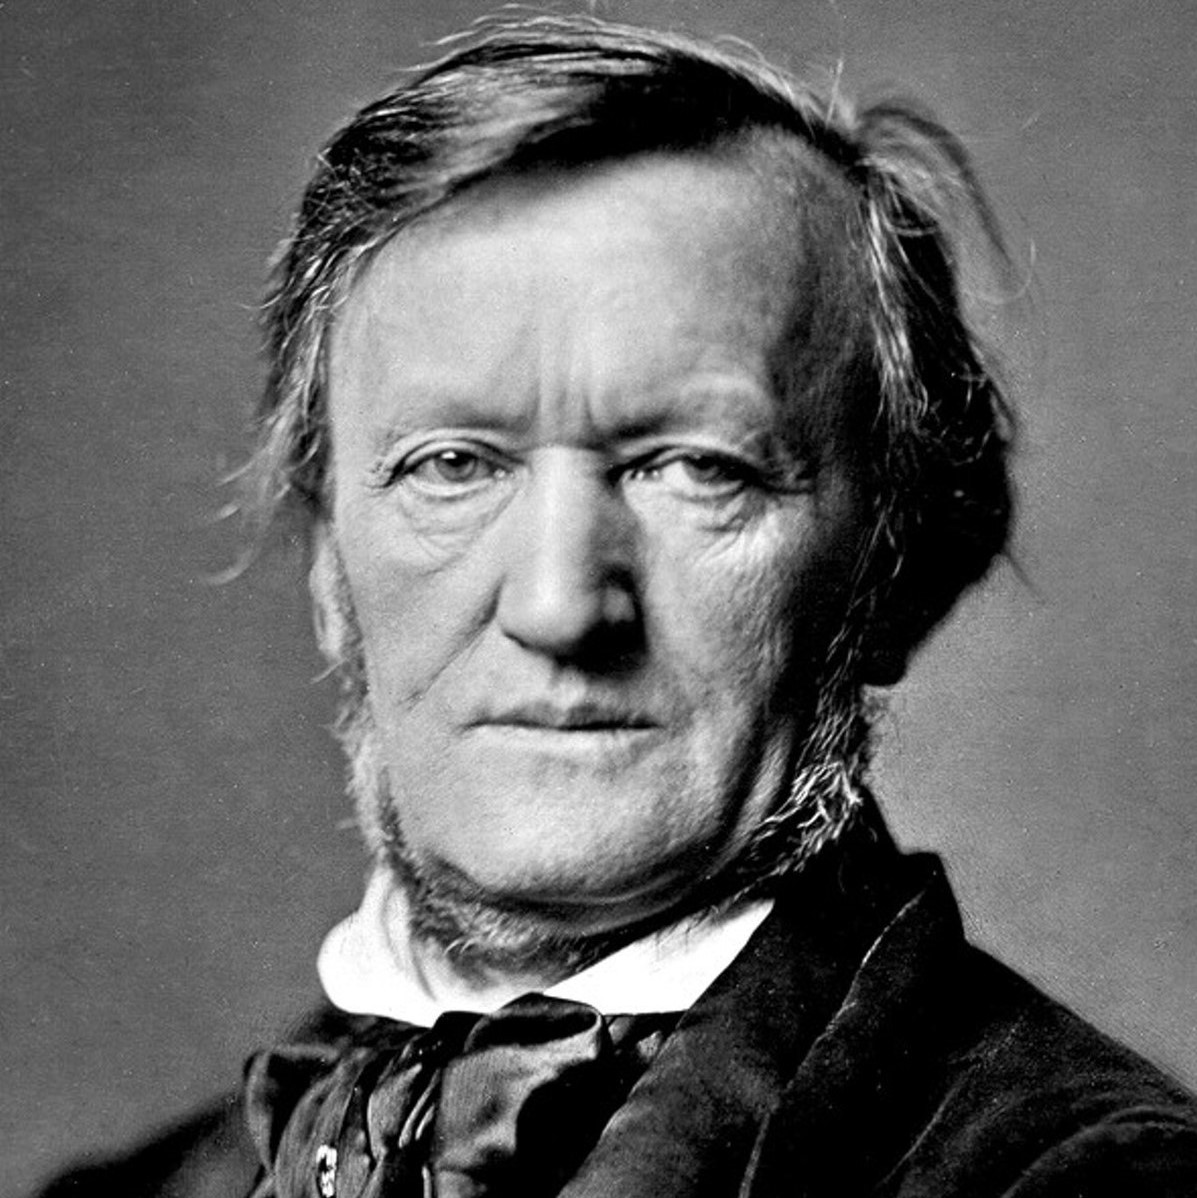
\includegraphics[width=5cm]{Richard_Wagner.jpg}\\
\caption{Richard Wagner (1813\textemdash1883); figura tomada de \href{https://www.nationalgeographic.com.es/historia/actualidad/richard-wagner-nacimiento-y-muerte_7014}{National Geographic}.}
\end{center}
\end{figure}

La idea del \emph{Gesamtkunstwerk} la desarroll� alrededor de 1850, y la plasm� en su totalidad en su ciclo de cuatro �peras \href{https://www.youtube.com/watch?v=1PBhlPeTJ_g}{\textit{Der Ring des Nibelungen}}, estrenado en 1876. Wagner control� y cre� cada aspecto de la tetralog�a, desde la m�sica hasta el libreto, el vestuario y la escenograf�a. Incluso mand� crear su propia sala de conciertos en Bayreuth, el \emph{Festspielhaus}, para que el escenario se adecuara a sus ideas sobre el pensamiento y la cultura musical; v�ase~\cite{kinney}.

As�, a ojos de compositores posteriores, se hab�an agotado todas las posibilidades de la m�sica tonal, y quiz�s ya hab�a comenzado el viraje hacia el predominio de la disonancia con su abundante uso del cromatismo, como en el famoso primer acorde del drama musical \href{https://www.youtube.com/watch?v=SF4zN-Okonc}{\textit{Tristan und Isolde}} (1865). Consta de las notas fa-si-$\mbox{re\#}$-$\mbox{sol\#}$, y sus intervalos desde el fa son una cuarta aumentada, una sexta aumentada y una novena aumentada.

Despu�s de Wagner, otros compositores tambi�n estuvieron a las puertas de emancipar la disonancia, de desatarla de las ataduras que impon�a la tonalidad. Por ejemplo, el gran compositor Gustav Mahler consegu�a reflejar en sus sinfon�as dos realidades paralelas: tanto la delicada fragilidad de la tradici�n anterior como la inminencia de su ruptura. El ejemplo m�s claro es el \href{https://www.youtube.com/watch?v=vHyV8noUXC0}{Adagio} de su D�cima Sinfon�a, que contiene una disonancia con once de las doce notas de la escala crom�tica. Y es que, sin lugar a dudas, la tonalidad ya preve�a que iba a ser reemplazada.

\begin{figure}[h]
\begin{center}
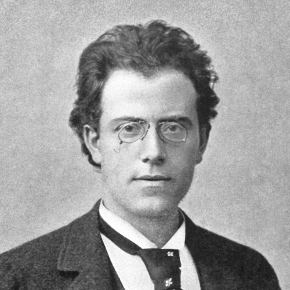
\includegraphics[width=5cm]{Gustav_Mahler.jpg}\\
\caption{Gustav Mahler (1860\textemdash1911); figura tomada de \href{http://www.planethugill.com/2018/09/mahler-distilled-iain-farrington-and.html}{Planet Hugill}.}
\end{center}
\end{figure}

Siguiendo la concepci�n del progreso como un camino ascendente, el paso siguiente para la composici�n musical deb�a consistir en deshacerse progresivamente de la tonalidad y desarrollar la ``{emancipaci�n de la disonancia}"  \textemdash mencionado tambi�n en \cite{scho} \emph{Composition with twelve tones}\textemdash. As�, en el marco expresionista del cambio de siglo, fue como Arnold Schoenberg ide� sus teor�as del pensamiento musical, y �stas dieron paso a la creaci�n de la atonalidad.

\subsection{Hacia el atonalismo de Schoenberg}
Fuertemente influido por Wagner y Mahler desde su adolescencia, Schoenberg comenz� componiendo al estilo posrom�ntico de su �poca, llevando el cromatismo y la orquestaci�n hasta el extremo. Sin embargo, y no espont�neamente, empez� a buscar en sus composiciones que cada sonido tuviera valor por s� mismo, un valor independiente de su funcionalidad tonal.

\begin{figure}[h]
\begin{center}
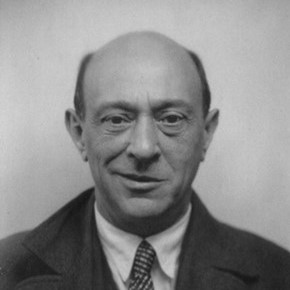
\includegraphics[width=5cm]{Arnold_Schoenberg.jpg}\\
\caption{Arnold Schoenberg (1874\textemdash1951); figura tomada de \href{http://es.nextews.com/59ce14c7/}{Nextews}.}
\end{center}
\end{figure}

Para �l, la m�sica no estaba intr�nsecamente dirigida a una t�nica. En las progresiones, lo importante era el paso de un acorde a otro, y no hacia d�nde se dirig�an estos. Adem�s, �l opinaba que se deb�an poder utilizar las notas de los modos eclesi�sticos libremente, por lo que consideraba las notas no diat�nicas tan v�lidas como las diat�nicas. Esto hac�a imposible distinguir unas de otras, y apenas se pod�a identificar la t�nica. De esta, y de otras muchas formas, Schoenberg consegu�a que la jerarqu�a tonal quedara desestabilizada~\cite{kinney}.

De esta �poca es su primera obra importante, \href{https://www.youtube.com/watch?v=vqODySSxYpc}{\emph{Verkl�rte Nacht}} ({\it Noche transfigurada}), Op. 4. Compuesto en 1899, este sexteto de cuerdas est� inspirado por el poema hom�nimo de Richard Dehmel. La m�sica, seg�n su autor, expresa el paseo de un hombre y una mujer en medio del abrazo de la naturaleza.  Aunque en la obra a�n prevalece la armon�a tradicional basada en acordes, Schoenberg sit�a al oyente en un terreno de indefinici�n tonal, no s�lo en el plano arm�nico sino tambi�n en el mel�dico. Adem�s, hace uso del acorde de novena invertido, inexistente hasta entonces y, por tanto, rechazado por la cr�tica~\cite{diaz}.

Tras pasar por la etapa tonal posrom�ntica, y debido a su convicci�n en la inexorabilidad de la evoluci�n de la m�sica hacia el cromatismo total, en 1908 Schoenberg se deslig� de la tonalidad completamente con el ciclo de canciones \href{https://www.youtube.com/watch?v=3iXsKhaZB2Q}{\emph{Das Buch der H�ngenden G�rten}}. 

A partir de entonces se dedic� a componer fragmentos muy breves cuya estructura era definida por motivos y no por la armon�a. Era esto lo que sol�a ocurrir en formas musicales anteriores como la forma sonata. A este periodo en sus composiciones se le llama atonalidad libre, aunque cabe destacar que Schoenberg rechazaba fervientemente este t�rmino:

\begin{quote}
\emph{La expresi�n ``m�sica atonal'' es de lo m�s desafortunada \textemdash es como llamar a volar ``el arte de no caer'' o nadar ``el arte de no ahogarse''.}\\
{\footnotesize Mencionado en \cite{hauer} A. Schoenberg, \emph{Hauer's Theories}, en \emph{Style and Idea}, 1923.}
\end{quote}

\noindent A este periodo pertenece tambi�n su famoso ciclo de canciones \href{https://www.youtube.com/watch?v=vQVkbKULKpI}{\emph{Pierrot Lunaire}}, Op. 21 (1912). Su nombre completo es \textit{Tres veces siete poemas de Pierrot Lunaire de Albert Giraud}, ya que est� dividida en 3 grupos de 7 canciones cada uno, cuyos textos son una selecci�n de 21 poemas del ciclo hom�nimo de Albert Giraud. 

Se encuentran en ella abundantes referencias al n�mero 7. Schoenberg hace un uso extensivo de motivos de 7 notas a lo largo de la obra, mientras que el conjunto musical que la interpreta, incluyendo al director, consta de 7 miembros. De hecho, a este conjunto de instrumentos \textemdash flauta, clarinete, viol�n, violonchelo, piano y voz\textemdash~se le ha dado el nombre de \textit{ensemble Pierrot} en su honor.  Otros n�meros importantes en la obra son el 3 y el 13. Cada poema consta de 13 l�neas, mientras que la primera l�nea de cada poema aparece 3 veces: en las l�neas 1, 7 y 13.

En esta obra no s�lo hay una ausencia total de relaciones tonales, sino que el tratamiento vocal evita tambi�n cualquier relaci�n est�tica con las t�cnicas tradicionales: es un \emph{Sprechgesang}, un canto hablado. De hecho, Schoenberg se refiere a estas piezas no como canciones, sino como melodramas. V�ase~\cite{diaz} para m�s informaci�n.

\subsection{El surgimiento del sistema dodecaf�nico}
Schoenberg no estaba a�n satisfecho con su t�cnica compositiva, ya que admiraba las obras extensas de los m�sicos rom�nticos y pensaba que su atonalidad no pod�a sostener una obra de gran envergadura. Es decir, necesitaba un hilo conductor mejor que los motivos para poder componer obras atonales m�s largas.

Por aquella �poca sufri� crisis en varios aspectos de su vida. En lo personal, su mujer Matilde Zemlinsky acababa de abandonarlo por otro hombre, aunque posteriormente volver�a junto al compositor. Y en lo profesional, sus obras no eran del gusto del p�blico, por lo que no contaba con suficiente dinero para mantener a su familia. Todas estas circunstancias, unidas al desarrollo de la Primera Guerra Mundial, no le permitieron componer apenas entre 1914 y 1923.

Tras el final de la guerra, en 1919, Schoenberg fund� la Sociedad para Interpretaciones Musicales Privadas junto a sus disc�pulos y amigos Alban Berg y Anton Webern. Schoenberg, Berg y Webern se autodenominaron la Segunda Escuela de Viena en honor al grupo de compositores del siglo XVIII Haydn, Mozart y Beethoven, quienes formaban la Primera Escuela de Viena.

En la Sociedad para Interpretaciones Musicales Privadas se presentaban m�sicas contempor�neas en circunstancias que favorecieran su adecuada apreciaci�n. As� se evitaba que dichas obras, al no ser entendidas por el p�blico, fueran inmediatamente rechazadas. Las obras de compositores como Mahler, Debussy, Bart�k, Ravel, Strauss y Stravinsky fueron incluidas en los programas de conciertos organizados por la Sociedad.

En este contexto Schoenberg pudo reflexionar sobre sus t�cnicas compositivas, y al fin public� en 1923 su ensayo \emph{M�todo de composici�n con doce sonidos}~\cite{scho}, donde se describ�an por primera vez los axiomas del dodecafonismo. Estos axiomas constitu�an la soluci�n al problema de la atonalidad libre que tanto le hab�a estado atormentando durante una d�cada.

Su primera obra �ntegramente dodecaf�nica, publicada tambi�n en 1923, es la Suite para piano Op. 25, que podr�n ver a continuaci�n. Es la pieza m�s temprana en la que Schoenberg usa series dodecaf�nicas en cada uno de los movimientos. En dos obras anteriores a ella usa series dodecaf�nicas, pero en movimientos aislados: la Op. 23, \href{https://www.youtube.com/watch?v=7A9HSlgDlQE}{\emph{5 St\"ucke}} (1920\textemdash23), en el movimiento de Waltz final; y su \href{https://www.youtube.com/watch?v=fzAFalLbXxg}{Serenata}, Op. 24, en su Soneto central.

Las series utilizadas en la Suite Op. 25 servir�n de ejemplo en este texto, y su tercer movimiento, \href{https://www.youtube.com/watch?v=scwNtGdop6w}{Musette}, ser� estudiado y analizado en el apartado \ref{musette} con el fin de entender una obra dodecaf�nica en toda su extensi�n. A continuaci�n el lector podr� escuchar la Suite para piano Op. 25:

\xxx{Incluir v�deo}
    \chapter[EL SISTEMA DODECAFÓNICO DE SCHOENBERG]{EL SISTEMA DODECAFÓ- NICO DE SCHOENBERG}
	\section{Los postulados del dodecafonismo}
		El dodecafonismo es un sistema compositivo que predetermina la melodía y la armonía a partir de una ordenación de las doce notas de la escala cromática, que se llama \textit{serie}. Ésta y algunas de sus transformaciones son los ladrillos con los que se construyen las alturas de las notas; son el único material que se puede utilizar. \cite{delgado}
		
		El resto de elementos de la pieza, como el número de instrumentos, el ritmo, el carácter, la textura o las dinámicas, se dejan a discreción del compositor. No serializar todos los conjuntos será la principal crítica al dodecafonismo por parte de los compositores serialistas que sucedieron a su creador, Arnold Schoenberg. Para los serialistas integrales, como Pierre Boulez, aquello restaba cohesión al modelo compositivo; para los dodecafonistas, aportaba libertad. \cite{boulez}
		
		Precisamente la predeterminación dodecafónica, aunque parece limitante, permite realizaciones musicales y estilos de composición muy diferentes: Schoenberg daba un tratamiento tradicional a sus obras, ya que aún admiraba las formas clásicas; Alban Berg iba más allá al utilizar series que recordaban a las tríadas tonales; y, en cambio, Anton Webern evitaba radicalmente cualquier asociación con la tradición. \cite{delgado}
		
		Schoenberg definió su sistema musical a partir de cuatro postulados que, en realidad, se basan en principios matemáticos \cite{dominguez}:
		
		\emph{1. La serie \emph{[sobre la que se construye la obra dodecafónica]} consta de las doce notas de la escala cromática dispuestas en un orden lineal específico.}
		
		\emph{2. Ninguna nota aparece más de una vez en la serie.}
		
		Los dos primeros postulados expresan que una obra dodecafónica fundamenta su estructura sobre una permutación de la escala de doce semitonos. Dicha permutación $\sigma$ es una biyección del conjunto numerado de las doce notas \{Do = 0, Do\# = 1, Re = 2, Re\# = 3, Mi = 4, Fa = 5, F\# = 6, Sol = 7, Sol\# = 8, La = 9, La\# = 10, Si = 11\} consigo mismo, y se representa de esta forma:
		
		\full{
			\drow{
				\sigma(0),\sigma(1),\sigma(2),\sigma(3),\sigma(4),\sigma(5),\sigma(6),\sigma(7),\sigma(8),\sigma(9),\sigma(10),\sigma(11)
			}
		}
	
		La permutación $\sigma(m)$, con $m\in \mathbb{Z} / (12)$\footnote{$\mathbb{Z} / (12)=\{0,\ 1,\ 2,\ 3,\ 4,\ 5,\ 6,\ 7,\ 8,\ 9,\ 10,\ 11\}$}, pertenece al grupo simétrico de orden 12: $\sigma\in$ S$_{12}$. Por ejemplo, en la Suite para piano Op. 25 Schoenberg utiliza como serie original en todos los movimientos de la obra la siguiente permutación $\sigma$:
		
		\[\sigma=\drow{4,5,7,1,6,3,8,2,11,0,9,10}\]	
		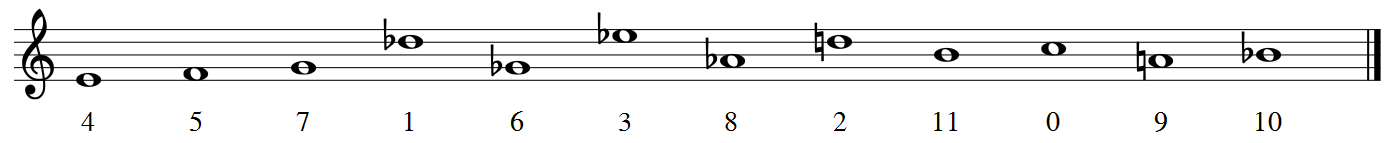
\includegraphics[width=\textwidth]{1.png}
		
		\emph{3. La serie será expuesta en cualquiera de sus aspectos lineales: original, inversión, retrogradación de la original y retrogradación de la inversión.}
		 
		\emph{4. La serie puede usarse en sus cuatro aspectos desde cualquier nota de la escala.}
		
		Los dos últimos postulados amplían los recursos compositivos al admitir la transformación de la serie original mediante \emph{inversión}, \emph{retrogradación}, \emph{inversión retrógrada} y \emph{transposición}\footnote{No confundir con un 2-ciclo. Una transposición musical se corresponde con una traslación matemática.}. El compositor puede utilizar cualquiera de las transformaciones de una serie al componer su obra dodecafónica. El conjunto de series que puede utilizar, que viene dado por la serie original y todas sus posibles transformaciones, se conoce como \emph{espectro serial}. \cite{dominguez}
		
	\section{Las transformaciones de una serie}
		\label{transPsi}
		Transformar una serie es matemáticamente equivalente a aplicar una función sobre la serie, y que asocie esa permutación a la permutación transformada. Por tanto, cualquier función transformativa $\Psi$ se aplica sobre el conjunto de las permutaciones, S$_{12}$.
		
	\subsection{Transposiciones}
		La \emph{transposición}, mencionada en el cuarto postulado, consiste en subir o bajar la serie original un número determinado de semitonos. Por tanto, no se modifican los intervalos entre las notas, sino solamente la altura a la que está la serie. Ya que consideraremos todas las octavas equivalentes, debemos trabajar módulo 12. 
		
		La serie transportada k semitonos (con k constante), T$^\text{k}\left(\sigma\right)$, se construye sumando k a $\sigma$ (mod. 12):
		\[\text{T}^\text{k}\left(\sigma\left(m\right)\right)=\sigma\left(m\right)+\text{k}\]		
		\full{$
		\text{T}^\text{k}=
		\left(\begin{matrix}
			0&1&2&&9&10&11\\
			\sigma\left(0\right)+\text{k}&\sigma\left(1\right)+\text{k}&\sigma\left(2\right)+\text{k}&
			\cdots&
			\sigma\left(9\right)+\text{k}&\sigma\left(10\right)+\text{k}&\sigma\left(11\right)+\text{k}\\
		\end{matrix}\right)
		$}
		
		A su vez, T$^\text{k}$ se forma al componer k transposiciones de 1 semitono: $\text{T}^\text{k}=\text{T}^1\circ\text{T}^1\circ\ldots\circ\text{T}^1$, k veces. Debido a que k es en realidad el exponente en la potencia de T, se coloca este número como superíndice.
		
		Históricamente, la notación $\Psi_\text{k}$, $\Psi^\text{k}$ o $\Psi(\text{k})$ se ha usado en sustitución de la composición de la transposición T$^\text{k}$ y otra función $\Psi$, en el respectivo orden: $\Psi^\text{k}=\Psi \circ \text{T}^\text{k} = \Psi(\text{T}^\text{k})$. Sin embargo, esta notación es especialmente ambigua y confusa, sobre todo al trabajar con funciones no conmutativas. Por ello, es preferible ceñirse a la notación estrictamente matemática; es decir, a la composición de funciones, aun omitiendo $\circ$: \cancel{$\Psi_\text{k}$}, \cancel{$\Psi^\text{k}$}, \cancel{$\Psi(\text{k})$} $\rightarrow \Psi\text{T}^\text{k}$
		
		Una posible serie transportada sobre la permutación $\sigma$ de la Suite para piano Op. 25, con k $= 6$, es la siguiente serie T$^6$:
		\[\text{T}^6=\drow{10,11,1,7,0,9,2,8,5,6,3,4}\]	
		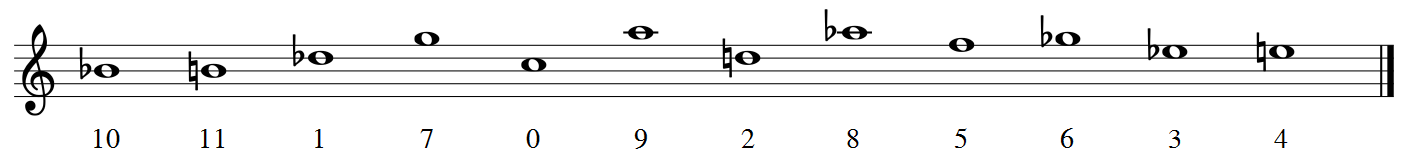
\includegraphics[width=\textwidth]{2.png}
		
	\subsection{Retrogradación}
		La \emph{retrogradación} consiste en leer la serie original desde la nota final hacia atrás, es decir, aplicar a la serie una simetría especular. De este modo, la primera nota irá al último puesto, la segunda al penúltimo, y así sucesivamente.
		
		La serie retrógrada se construye de esta forma:
		\[\text{R}\left(\sigma\left(m\right)\right)=\sigma\left(-1-m\right)\]
		\full{$\text{R}=\drow{\sigma(11),\sigma(10),\sigma(9),\sigma(8),\sigma(7),\sigma(6),\sigma(5),\sigma(4),\sigma(3),\sigma(2),\sigma(1),\sigma(0)}$}
			
		La serie retrógrada sobre la permutación $\sigma$ de la Suite Op. 25 es la siguiente serie R:	
		\[\text{R}=\drow{10,9,0,11,2,8,3,6,1,7,5,4}\]		
		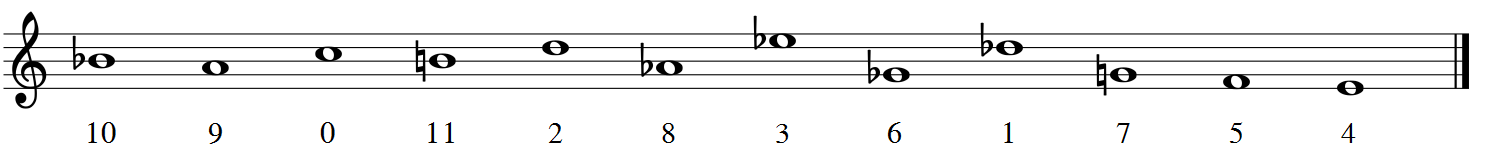
\includegraphics[width=\textwidth]{3.png}
		
	\subsection{Inversión}
		La \emph{inversión} consiste en cambiar la dirección --de ascendente a descendente, y viceversa-- de los intervalos entre cada nota de la serie. Si el primer intervalo en la serie original $\sigma$ es de $+k$, el primer intervalo en la serie invertida I será de $-k$ (mod. 12), por lo que debemos cambiar el signo de $\sigma$ para construir I. Además, queremos que la primera nota de ambas series, I(0) y $\sigma$(0), coincidan, así que debemos transportar la serie ($-\sigma$) un número $\lambda$ de semitonos para que esta condición se cumpla:
		\begin{align*}
		\text{I}(0)=-\sigma\left(0\right)+\lambda&=\sigma\left(0\right)\\
		\implies \lambda&=2\sigma(0)
		\end{align*}
		Por tanto, la serie invertida se construye de esta forma:
		\[\text{I}\left(\sigma\left(m\right)\right)=-\sigma\left(m\right)+2\sigma\left(0\right)\]
		\full{$
		\text{I}=\left(\begin{matrix}0&1&2&&10&11\\\sigma(0)&-\sigma(1)+2\sigma(0)&-\sigma(2)+2\sigma(0)&\ldots&-\sigma(10)+2\sigma(0)&-\sigma(11)+2\sigma(0)\\\end{matrix}\right)$}
		
		La serie invertida sobre la permutación $\sigma$ de la Suite Op. 25 es la siguiente serie I:
		\[\text{I}=\drow{4,3,1,7,2,5,0,6,9,8,11,10}\]		
		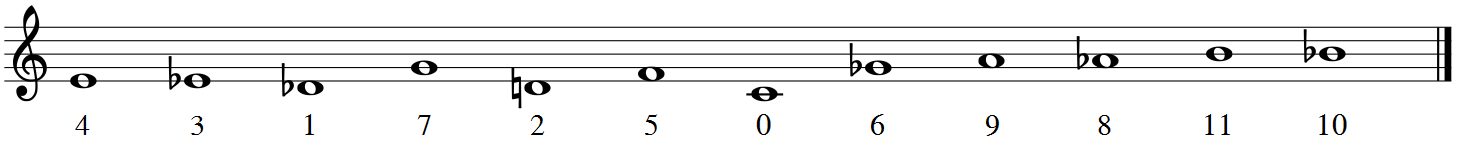
\includegraphics[width=\textwidth]{4.png}
				
		En total, obtendremos 48 series -- aunque no obligatoriamente distintas entre sí -- pertenecientes a un solo espectro serial. Hay 12 series originales sobre cada una de las doce notas, 12 series retrógradas, 12 invertidas y 12 series sobre las que se aplica tanto la retrogradación como la inversión. A continuación se muestra la sintaxis simple junto a la matemática:
		
		\begin{multicols}{2}
			\underline{Sintaxis simple}
			
			T$_0$, T$_1$, T$_2$\ldots
			
			R$_0$, R$_1$, R$_2$\ldots
			
			I$_0$, I$_1$, I$_2$\ldots
			
			IR$_0$, IR$_1$, IR$_2$\ldots
			
			\underline{Sintaxis matemática}
			
			T$^0$, T$^1$, T$^2$\ldots
			
			R, RT$^1$, RT$^2$\ldots
			
			I, IT$^1$, IT$^2$\ldots
			
			IR, IRT$^1$, IRT$^2$\ldots
		\end{multicols}
	
	\section{Matrices dodecafónicas}
		
		Dada una serie, su matriz dodecafónica es una representación visual de su espectro serial; es decir, del conjunto de series derivadas de esa serie. El espectro serial es todo el material compositivo sonoro del que se dispone para la composición de una obra dodecafónica. Al poder ordenar y disponer la información en una tabla, el compositor puede acceder a toda ella al mismo tiempo sin tener que calcular cada serie individualmente.		
		
		La matriz se lee en la dirección en la que aparece el nombre de la serie. Las series T se leen de izquierda a derecha, mientras que las series R de derecha a izquierda. Las series I se leen de arriba a abajo y las IR/RI de abajo a arriba.
		
		He creado un programa que devuelve en formato \LaTeX{} la matriz correspondiente a cualquier serie dodecafónica que se introduzca en teclado, además de producir la nomenclatura simple para cada serie. El código, escrito en C++, está incluido en el Anexo \ref{app:matrices}, página \pageref{app:matrices}.
		
		A continuación, se incluye la matriz dodecafónica de la serie P de la Suite Op. 25 de Schoenberg. Mientras que la mayoría de tablas tienen dos filas inferiores, que se corresponden con las distintas nomenclaturas de RI e IR para una misma serie – ya que normalmente no conmutan –, en la matriz de la serie P sí coinciden, como se mencionará en el apartado \ref{conmut}.
		
		\full{$\begin{array}{l|cccccccccccc|r}
		&\text{I}_{0}&\text{I}_{1}&\text{I}_{3}&\text{I}_{9}&\text{I}_{2}&\text{I}_{11}&\text{I}_{4}&\text{I}_{10}&\text{I}_{7}&\text{I}_{8}&\text{I}_{5}&\text{I}_{6}&\\
		\hline
		\text{T}_{0}&4&5&7&1&6&3&8&2&11&0&9&10&\text{R}_{0}\\
		\text{T}_{11}&3&4&6&0&5&2&7&1&10&11&8&9&\text{R}_{11}\\
		\text{T}_{9}&1&2&4&10&3&0&5&11&8&9&6&7&\text{R}_{9}\\
		\text{T}_{3}&7&8&10&4&9&6&11&5&2&3&0&1&\text{R}_{3}\\
		\text{T}_{10}&2&3&5&11&4&1&6&0&9&10&7&8&\text{R}_{10}\\
		\text{T}_{1}&5&6&8&2&7&4&9&3&0&1&10&11&\text{R}_{1}\\
		\text{T}_{8}&0&1&3&9&2&11&4&10&7&8&5&6&\text{R}_{8}\\
		\text{T}_{2}&6&7&9&3&8&5&10&4&1&2&11&0&\text{R}_{2}\\
		\text{T}_{5}&9&10&0&6&11&8&1&7&4&5&2&3&\text{R}_{5}\\
		\text{T}_{4}&8&9&11&5&10&7&0&6&3&4&1&2&\text{R}_{4}\\
		\text{T}_{7}&11&0&2&8&1&10&3&9&6&7&4&5&\text{R}_{7}\\
		\text{T}_{6}&10&11&1&7&0&9&2&8&5&6&3&4&\text{R}_{6}\\
		\hline
		&\text{IR}_{0}&\text{IR}_{1}&\text{IR}_{3}&\text{IR}_{9}&\text{IR}_{2}&\text{IR}_{11}&\text{IR}_{4}&\text{IR}_{10}&\text{IR}_{7}&\text{IR}_{8}&\text{IR}_{5}&\text{IR}_{6}&\\
		\hline
		&\text{RI}_{0}&\text{RI}_{1}&\text{RI}_{3}&\text{RI}_{9}&\text{RI}_{2}&\text{RI}_{11}&\text{RI}_{4}&\text{RI}_{10}&\text{RI}_{7}&\text{RI}_{8}&\text{RI}_{5}&\text{RI}_{6}&
		\end{array}$}
	
		Por otro lado, he escrito otro programa en el propio lenguaje \LaTeX{} que crea esta misma tabla con el comando \verb|\dmatrix|, y tiene cualquier serie como argumento: \verb|\dmatrix{4,5,7,1,6,3,8,2,11,0,9,10}|. El código se encuentra en el Anexo \ref{app:latex}, página \pageref{app:latex1}. La tabla aparece sin el orlado de nomenclaturas:
		\dmatrix{4,5,7,1,6,3,8,2,11,0,9,10}
	
		
		\bigbreak
		
		También he creado una página interactiva que genera matrices de cualquier serie para cualquier longitud serial, además de generar series aleatorias. Permite escoger entre dos numeraciones y dos nomenclaturas. Está escrita en Elm y el código puede encontrarse en \url{https://gitlab.com/dodecafonismo/matrices}.
		
		\begin{wrapfigure}{l}{0.2\textwidth}
			\vspace{-\bigskipamount}
			\qrcode{https://matrices.netlify.com/}
		\end{wrapfigure} En el código QR está el enlace de la aplicación web. Sus instrucciones de uso se encuentran al final de la página. El enlace es \url{https://matrices.netlify.com/}.
		
	\section{An�lisis de una obra dodecaf�nica: el opus 25}\label{ch:suite}
	\subsection{Series de la Suite op. 25}
		Lo primero que har� un compositor dodecaf�nico antes de empezar a componer ser� escoger su serie original. Su elecci�n nunca es una simple cuesti�n de azar; al contrario, ya que las singularidades de la serie dar�n un car�cter especial a toda la obra. Por ejemplo, el compositor puede escoger una serie con simetr�as, y as� tendr� series repetidas entre su espectro serial. Tambi�n puede tener simetr�as internas solo en un fragmento de tres o cuatro notas, y de este modo podr� el compositor oscilar entre varias series del espectro que se parezcan entre s�. Para un estudio m�s completo de las relaciones de similitud entre series se recomienda \emph{On the Similarity of Twelve-Tone Rows}, de Tuukka Ilom�ki \cite{ilomaki}.
		
		En la Suite para Piano Op. 25, Schoenberg escoge su serie $\sigma$ para resaltar el intervalo de tritono (6 semitonos). A continuaci�n se observan en negrita los intervalos entre las notas de esta serie, en unidad de semitono:
		
		\[\left(\begin{array}{*{24}c}
		0&&1&&2&&3&&4&&5&&6&&7&&8&&9&&10&&11&\\
		4&\mathbf{1}&5&\mathbf{2}&7&\mathbf{6}&1&\mathbf{5}&6&\mathbf{9}&3&\mathbf{5}&8&\mathbf{6}&2&\mathbf{9}&11&\mathbf{1}&0&\mathbf{9}&9&\mathbf{1}&10&\mathbf{6}\end{array}\right)\]
				
		Presenta repeticiones triples de los intervalos de tritono (6), de sexta mayor (9) y de segunda menor o semitono (1): los intervalos m�s disonantes; una repetici�n doble de cuarta justa (5), y un intervalo de segunda mayor (2); adem�s de una consecuci�n de intervalos repetida: 9--1--9--1. Como se forma el intervalo de tritono al enlazar la serie original con una serie que empiece por la misma nota, se tiene en cuenta el intervalo de tritono (6) al final. En el dodecafonismo se evitan deliberadamente los intervalos de tercera mayor (4), ya que estos son la base de la eludida armon�a tonal. \label{serie25}
		
		El intervalo de tritono tiene la particularidad de no modificarse en la inversi�n y transportaci�n k = 6, por lo que estos intervalos aparecen en los lugares originales, mientras que en los procedimientos de retrogradaci�n y retrogradaci�n inversa ocupan sus lugares en retr�grado. En particular, Schoenberg utiliza entre los seis movimientos de la Suite solamente las ocho series de todo el espectro serial que cumplen estos requisitos: $T^0$, $T^6$, $I$, $IT^6$, $R$, $RT^6$, $RI$ y $RIT^6$, que podemos observar a continuaci�n:
		
		\chapter{Series de la Suite Op. 25}
	\label{app:series}
	
	\newpage
	$$\text{T}^0=\left(\begin{matrix}0&1&2&3&4&5&6&7&8&9&10&11\\4&5&7&1&6&3&8&2&11&0&9&10\\\end{matrix}\right)$$
	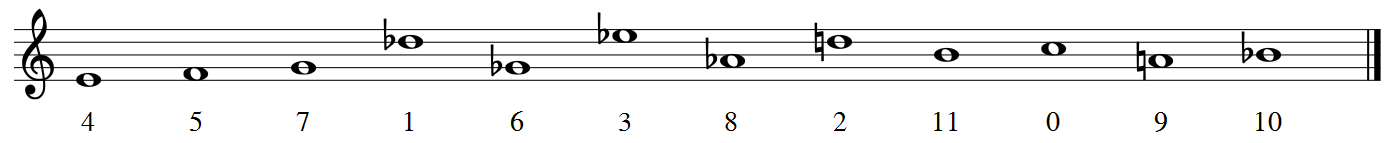
\includegraphics[width=\textwidth]{1.png}
	\bigskip\bigskip
	$$\text{T}^6=\left(\begin{matrix}0&1&2&3&4&5&6&7&8&9&10&11\\10&11&1&7&0&9&2&8&5&6&3&4\\\end{matrix}\right)$$
	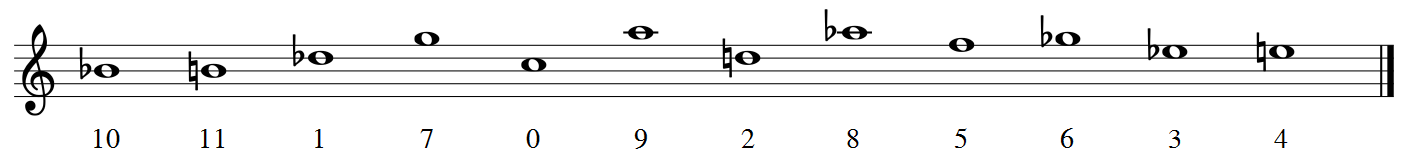
\includegraphics[width=\textwidth]{2.png}
	\bigskip\bigskip
	$$\text{IT}^0=\left(\begin{matrix}0&1&2&3&4&5&6&7&8&9&10&11\\4&3&1&7&2&5&0&6&9&8&11&10\\\end{matrix}\right)$$
	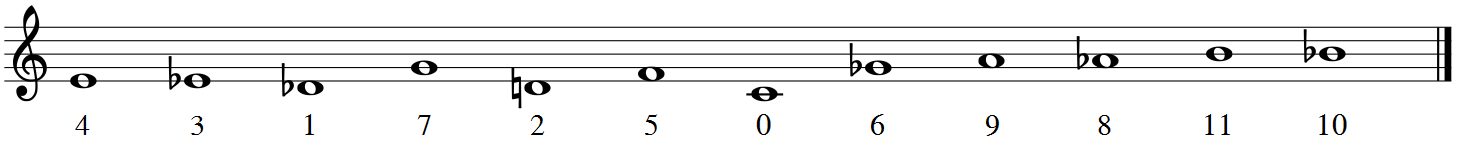
\includegraphics[width=\textwidth]{4.png}
	\bigskip\bigskip
	$$\text{IT}^6=\left(\begin{matrix}0&1&2&3&4&5&6&7&8&9&10&11\\10&9&7&1&8&11&6&0&3&2&5&4\\\end{matrix}\right)$$
	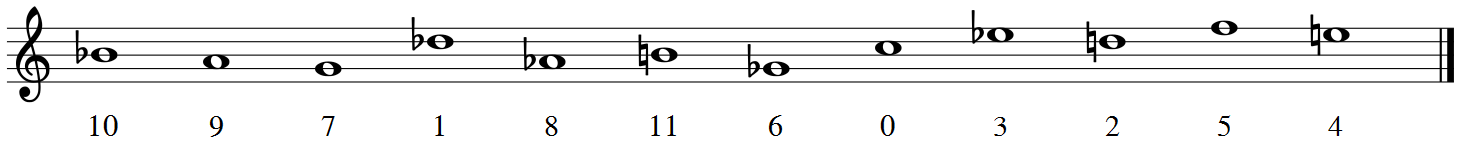
\includegraphics[width=\textwidth]{6.png}
	\newpage
	$$\text{RT}^0=\left(\begin{matrix}0&1&2&3&4&5&6&7&8&9&10&11\\10&9&0&11&2&8&3&6&1&7&5&4\\\end{matrix}\right)$$
	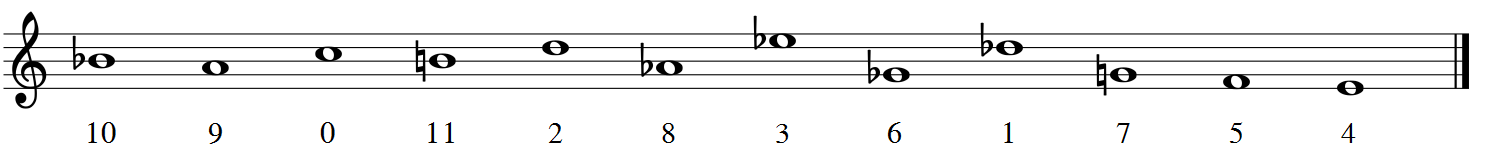
\includegraphics[width=\textwidth]{3.png}
	\bigskip\bigskip
	$$\text{RT}^6=\left(\begin{matrix}0&1&2&3&4&5&6&7&8&9&10&11\\4&3&6&5&8&2&9&0&7&1&11&10\\\end{matrix}\right)$$
	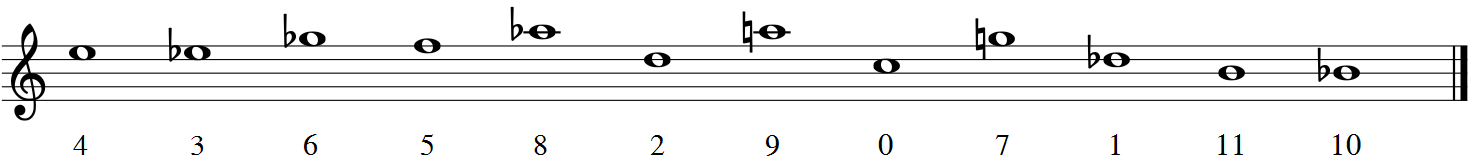
\includegraphics[width=\textwidth]{7.png}
	\bigskip\bigskip
	$$\text{IRT}^0=\left(\begin{matrix}0&1&2&3&4&5&6&7&8&9&10&11\\10&11&8&9&6&0&5&2&7&1&3&4\\\end{matrix}\right)$$
	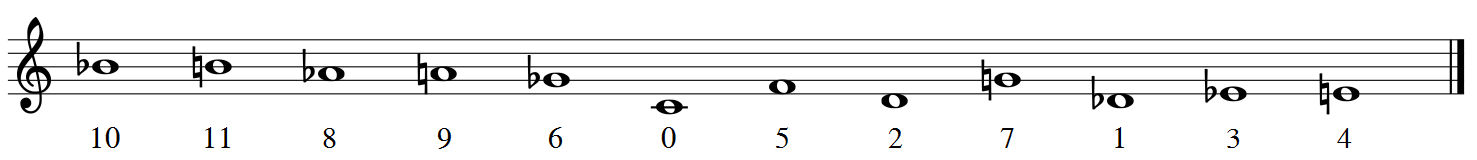
\includegraphics[width=\textwidth]{5.png}
	\bigskip\bigskip
	$$\text{IRT}^6=\left(\begin{matrix}0&1&2&3&4&5&6&7&8&9&10&11\\4&5&2&3&0&6&11&8&1&7&9&10\\\end{matrix}\right)$$
	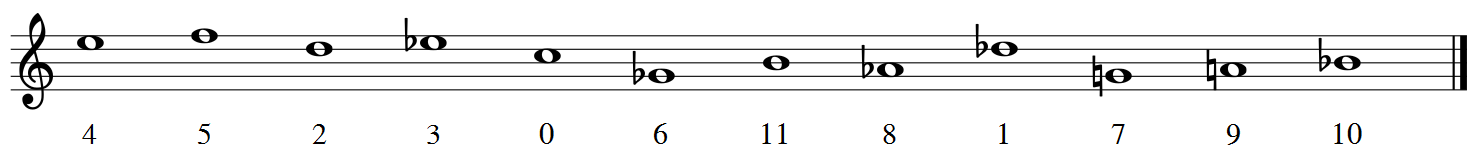
\includegraphics[width=\textwidth]{8.png}
		
		Estas series tienen muchos elementos en com�n: todas comienzan o acaban por mi$\natural$ o por si$\flat$, lo que permite enlazar unas series con otras por medio del un�sono o del tritono; se mantienen los intervalos de tritono en sus lugares originales o retr�grados, y coinciden en las dos primeras y las dos �ltimas notas dos a dos.
		
		Se han realizado estudios -- como el de Martha Hyde \cite{hyde} -- en los que se limitan las series utilizadas en la Suite a cuatro: $T^0$, $T^6$, $I$ e $IT^6$, pero ya que el objetivo de este texto no es analizar la obra entera se dejar� esta cuesti�n para an�lisis posteriores.
		
	\subsection{Descripci�n de la Suite op. 25}
		Schoenberg realiza en la serie $\sigma$ una partici�n triple; es decir, la serie se divide en tres tetracordios, y cada uno de ellos contiene un intervalo de tritono. El �ltimo tetracordio, si se retrograda, consta de las notas 10--9--0--11, que en notaci�n germ�nica es la secuencia BACH. Esto puede ser un homenaje al compositor Johann Sebastian Bach (1685\textemdash1750), ya que Schoenberg admiraba a los grandes compositores anteriores a �l por las estructuras formales de sus obras. Para m�s informaci�n, v�ase~\cite{xiao}.
		
		Otro posible homenaje a Bach y sus contempor�neos barrocos es precisamente la forma de la obra: es una Suite, g�nero cultivado durante los siglos XVII y XVIII que se compone de una variedad de danzas. La Suite de Schoenberg est� formada por seis danzas: un Preludio, una Gavota, una Musette, un Intermezzo \textemdash que no tiene influencia barroca sino m�s bien de Brahms, otro modelo para Schoenberg\textemdash, un Minueto con Tr�o y una Giga. Adem�s, el estilo, la textura \textemdash contrapunt�stica, t�picamente barroca\textemdash~ y la estructura de cada danza se corresponden con los estilos, texturas y estructuras de las danzas hom�nimas del periodo bachiano.
        
        Por ser �sta su primera obra totalmente dodecaf�nica, Schoenberg la utiliz� como una muestra al mundo de las posibilidades de su nuevo m�todo compositivo. Fue tambi�n por lo que tom� un formato tan variado como una Suite: as� pod�a en una misma obra componer con estilos tan distintos como los de las distintas danzas.
        
        Al componer la obra, Schoenberg trata cada tetracordio como una subunidad individual. Los superpone contra otras series del espectro tambi�n divididas, o utiliza sus notas como un solo acorde cuatr�ada. Estas divisiones no s�lo sirven para hacer la serie m�s reconocible o a�adir cohesi�n a la obra, sino que adem�s facilitan el desarrollo de la serie espec�ficamente en el estilo de cada danza.
		
	\subsection{An�lisis de la Musette}
	\label{musette}
		En el tercer movimiento de la Suite, la Musette, Schoenberg recrea la danza barroca que toma su nombre del instrumento hom�nimo: la \emph{cornamusa}, de la familia de la gaita. La m�sica compuesta para estos instrumentos suele consistir en una melod�a acompa�ada por una nota pedal, que se traduce aqu� en la presencia de un bord�n sobre el sol$\natural$ (nota 7). Esta nota se extrae de cada una de las series utilizadas y se forma con ella un ostinato r�tmico en la mano izquierda del piano. Con el resto de sonidos de cada serie, Schoenberg vuelve a emular el estilo de la danza barroca y articula un discurso polif�nico a dos voces con ritmos esencialmente cortos.
		
		A partir de la doble barra del comp�s 9, el re$\flat$ (nota 1) acompa�a a sol$\natural$ y ambos crean un doble bord�n en la mano izquierda. La elecci�n de esas dos notas est� estrechamente relacionada con la tradicional relaci�n de quinta justa formada por sol$\natural$ y re$\natural$ en la m�sica tonal. Schoenberg sustituye las quintas justas tonales por los tritonos dodecaf�nicos, subrayando a�n m�s su <<emancipaci�n de la disonancia>>.
		
		Adem�s de las similitudes texturales, r�tmicas y arm�nicas, la Musette de Schoenberg comparte estructura formal con las danzas barrocas. Y esta semejanza es quiz�s la m�s notable, ya que fue la b�squeda de estructura formal lo que inspir� a Schoenberg a desarrollar su m�todo compositivo. La Musette barroca, como todos los movimientos de danza, presenta una estructura binaria con simetr�a tonal: empieza y acaba por la misma tonalidad, mientras que el centro es zona de desarrollo. Schoenberg despoja de funcionalidad tonal a esa simetr�a, madre de la forma sonata, y la aplica a su composici�n dodecaf�nica.
		
		En este movimiento se pueden diferenciar a simple vista tres secciones, divididas en los compases 9 y 20, debido a cambios de textura, figuraci�n y tempo. En la segunda secci�n se le a�ade melod�a a la mano izquierda del piano, dejando m�s camuflado el bord�n que en la primera secci�n, adem�s de que �ste se vuelve doble, mientras que vuelve a aparecer claramente en la tercera secci�n. Tambi�n en la segunda secci�n aparece una nueva figuraci�n, que es la semicorchea; y, por �ltimo, en los dos compases de divisi�n aparecen dos \emph{a tempo}, que marcan el final de las dos primeras secciones tras dos zonas de variabilidad r�tmica.
		
		Para que esta estructura tr�ptica sea una forma binaria, la primera y la �ltima parte deben mantener un parecido, que se observa a trav�s del an�lisis de las series utilizadas en el movimiento. Estas series son $T^0$, $T^6$, $I$ e $IT^6$.
		
		En la Musette, Schoenberg hace un uso casi absoluto de la tripartici�n serial, hasta el punto de individualizar los tetracordios por separado y concederles privilegios seriales, como la retrogradaci�n. Por ejemplo, en el comp�s 7, en la voz inferior de la mano derecha aparece el tetracordio 4--5--2--3, que es o bien el primer tetracordio de $RIT^6$ o la retrogradaci�n del tercer tetracordio de $IT^6$, mientras que los otros dos tetracordios de $IT^6$, 10--9--7\footnote{La nota 7 aparece como bord�n y no en la misma voz que el resto del tetracordio, por lo que su posici�n es tambi�n excepcional.}--1 en la voz superior y 8--11--6--0 en la mano izquierda, aparecen en el orden correcto. Entonces no se puede analizar el comp�s como $RIT^6$, sino indicar que hay una alteraci�n puntual de $IT^6$.
		
		Por tanto, es muy complicado analizar esta obra en su totalidad, ya que la flexibilidad en la ordenaci�n de los tetracordios puede generar situaciones muy ambiguas. Debido a estas fragmentaciones y a las variadas combinaciones de tetracordios originales y retr�grados, se escucha un �rea de desarrollo hacia la secci�n media del movimiento. En cambio, las series al principio y al final de la pieza se presentan casi �ntegramente, como una exposici�n y reexposici�n. He aqu� un v�nculo con la simetr�a de las formas binarias tonales.
		
		Es m�s, incluso el orden de las series utilizadas en la primera y en la �ltima secci�n coinciden, exceptuando dos repeticiones consecutivas y las series $T^0$ finales, que act�an como una cadencia serial:
		
		\[\begin{array}{*{12}c}
			\mathbf{c}.\mathbf{1}&T^0&IT^6&T^6&I&T^0&I&T^6&
				\begin{matrix}IT^6&IT^6\\
				\end{matrix}
			&&&\mathbf{c}.\mathbf{9}\\
			\mathbf{c}.\mathbf{22}&T^0&IT^6&T^6&I&T^0&
				\begin{matrix}
				I&I\\
				\end{matrix}
			&T^6&IT^6&T^0&T^0&\mathbf{c}.\mathbf{31}\\\end{array}\]
		
		A continuaci�n se encuentra el an�lisis serial completo de la Musette:

\newpage
\begin{figure}[!h]
\begin{center}
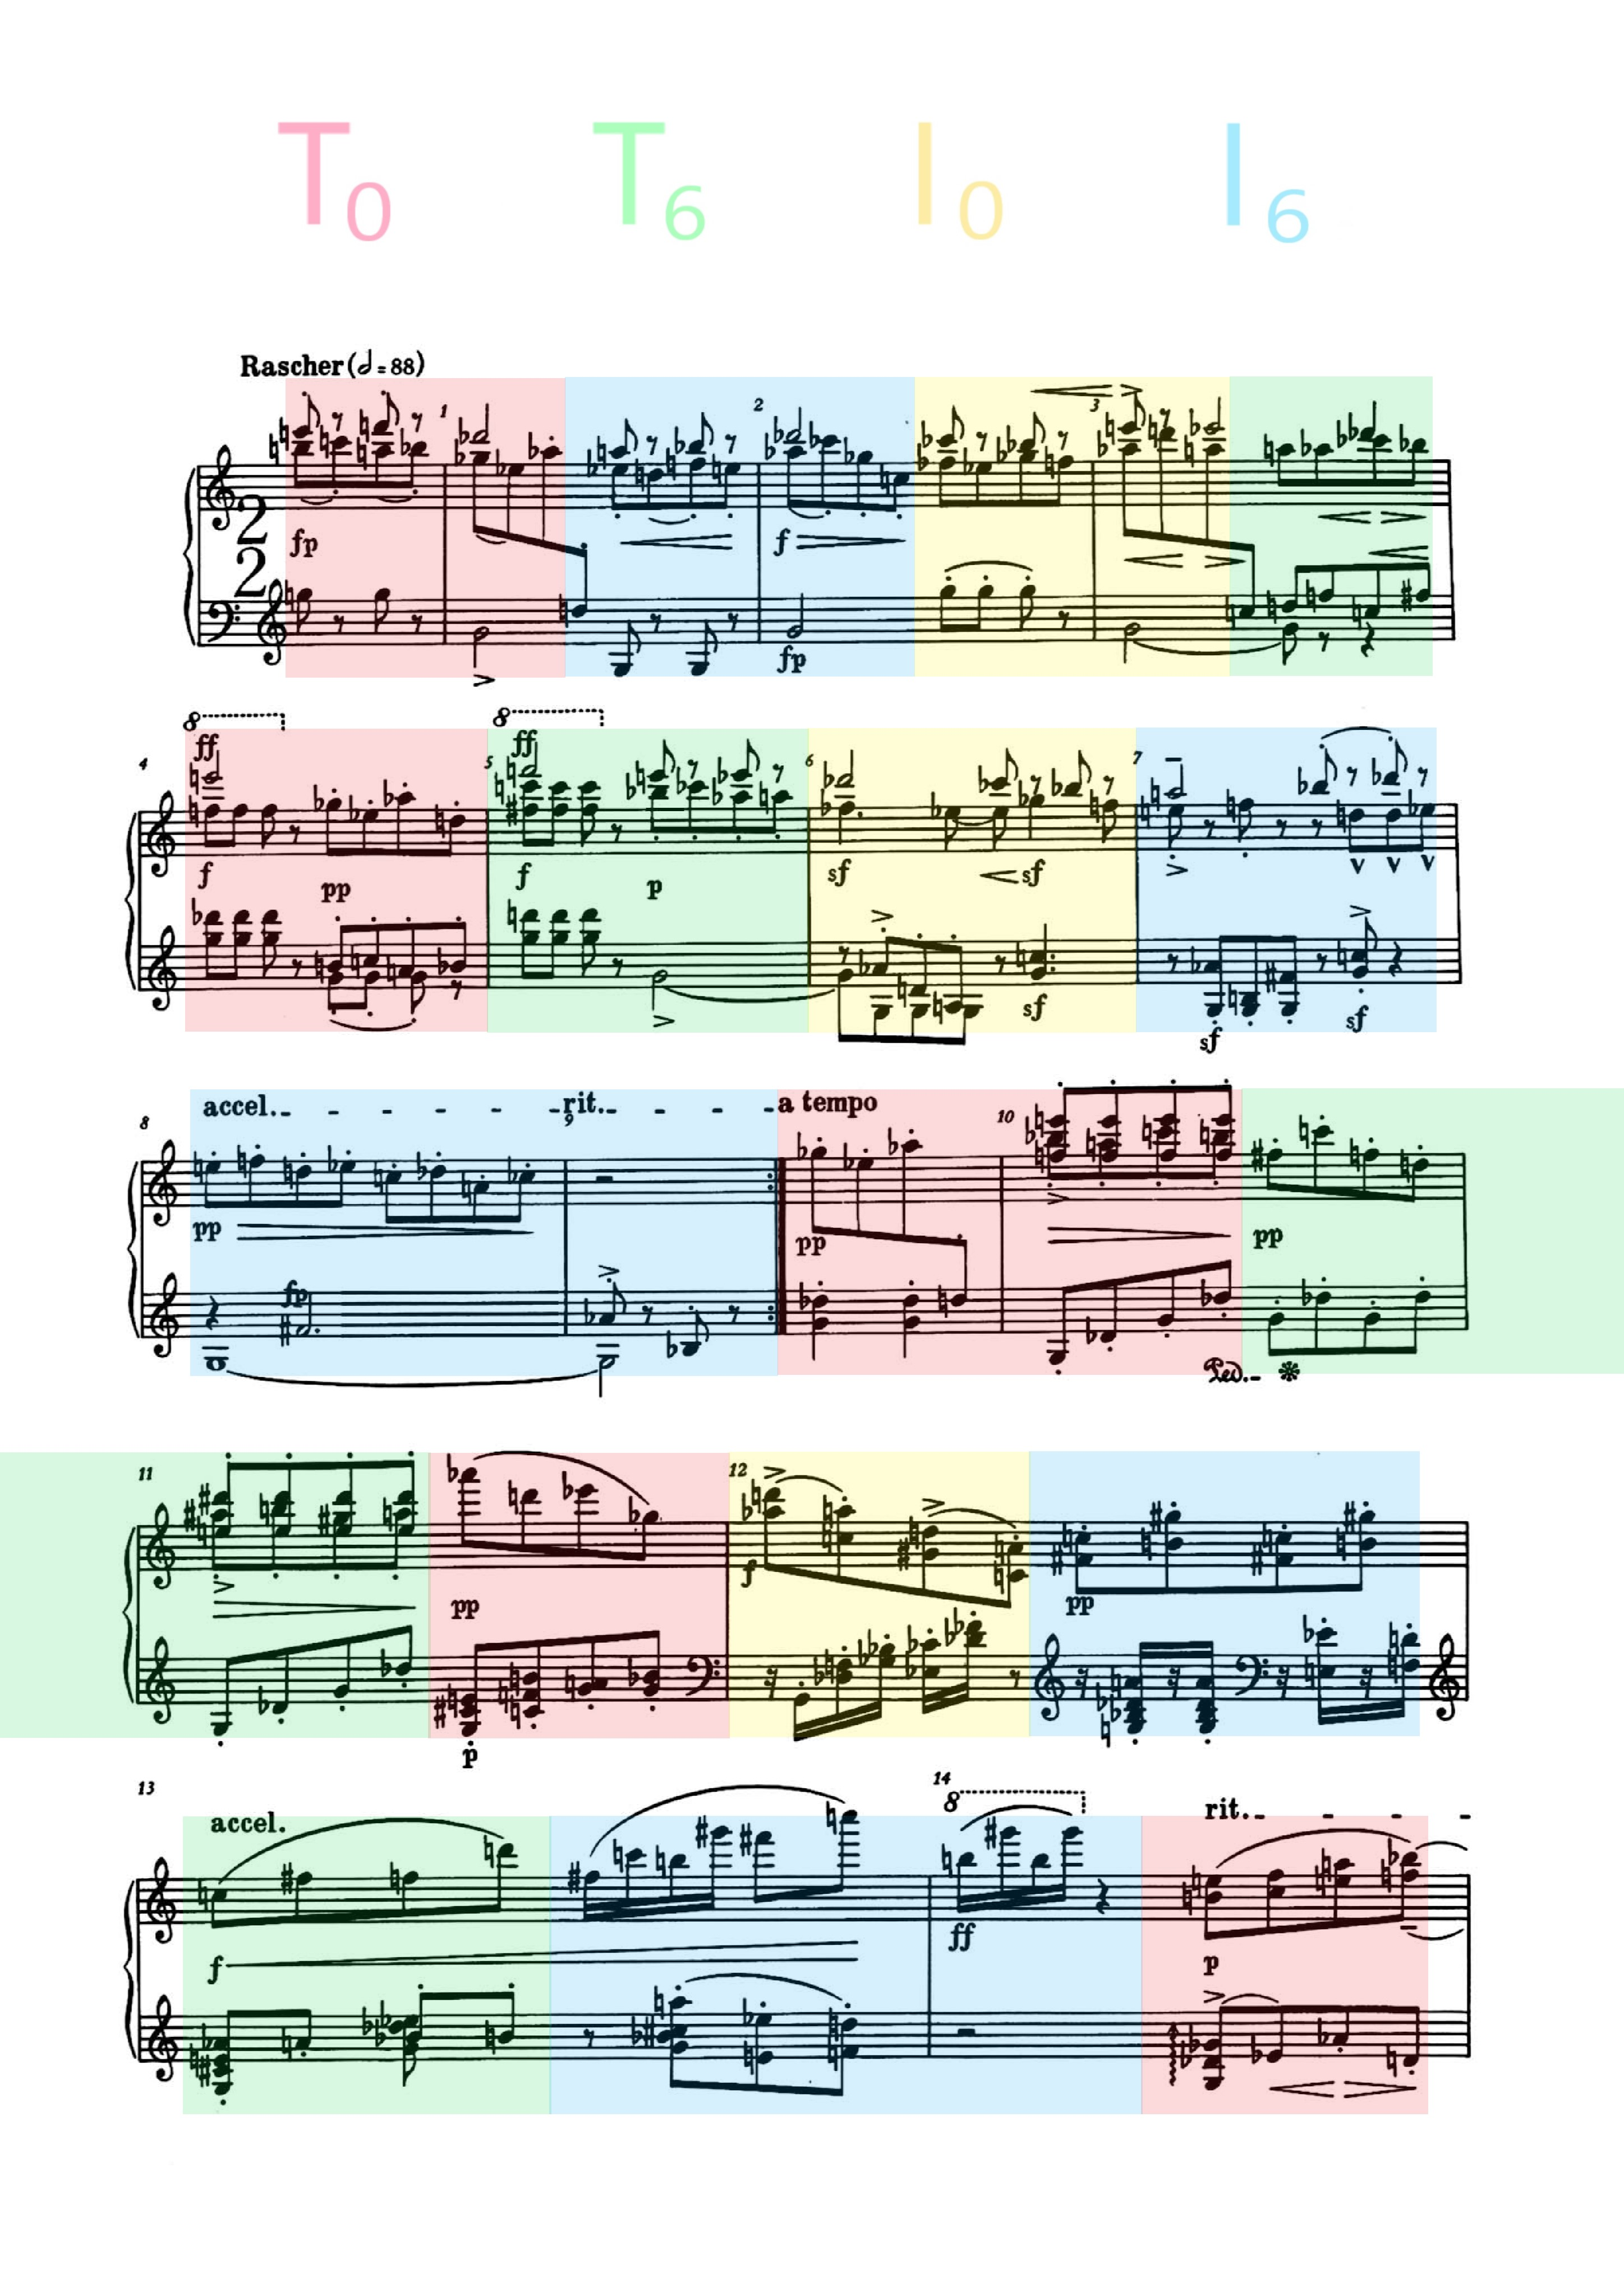
\includegraphics[width=14.5cm]{9.jpg}\\
\caption{An�lisis de la Musette (I)}
\end{center}
\end{figure}
$\,$


\newpage
\begin{figure}[!ht]
\begin{center}
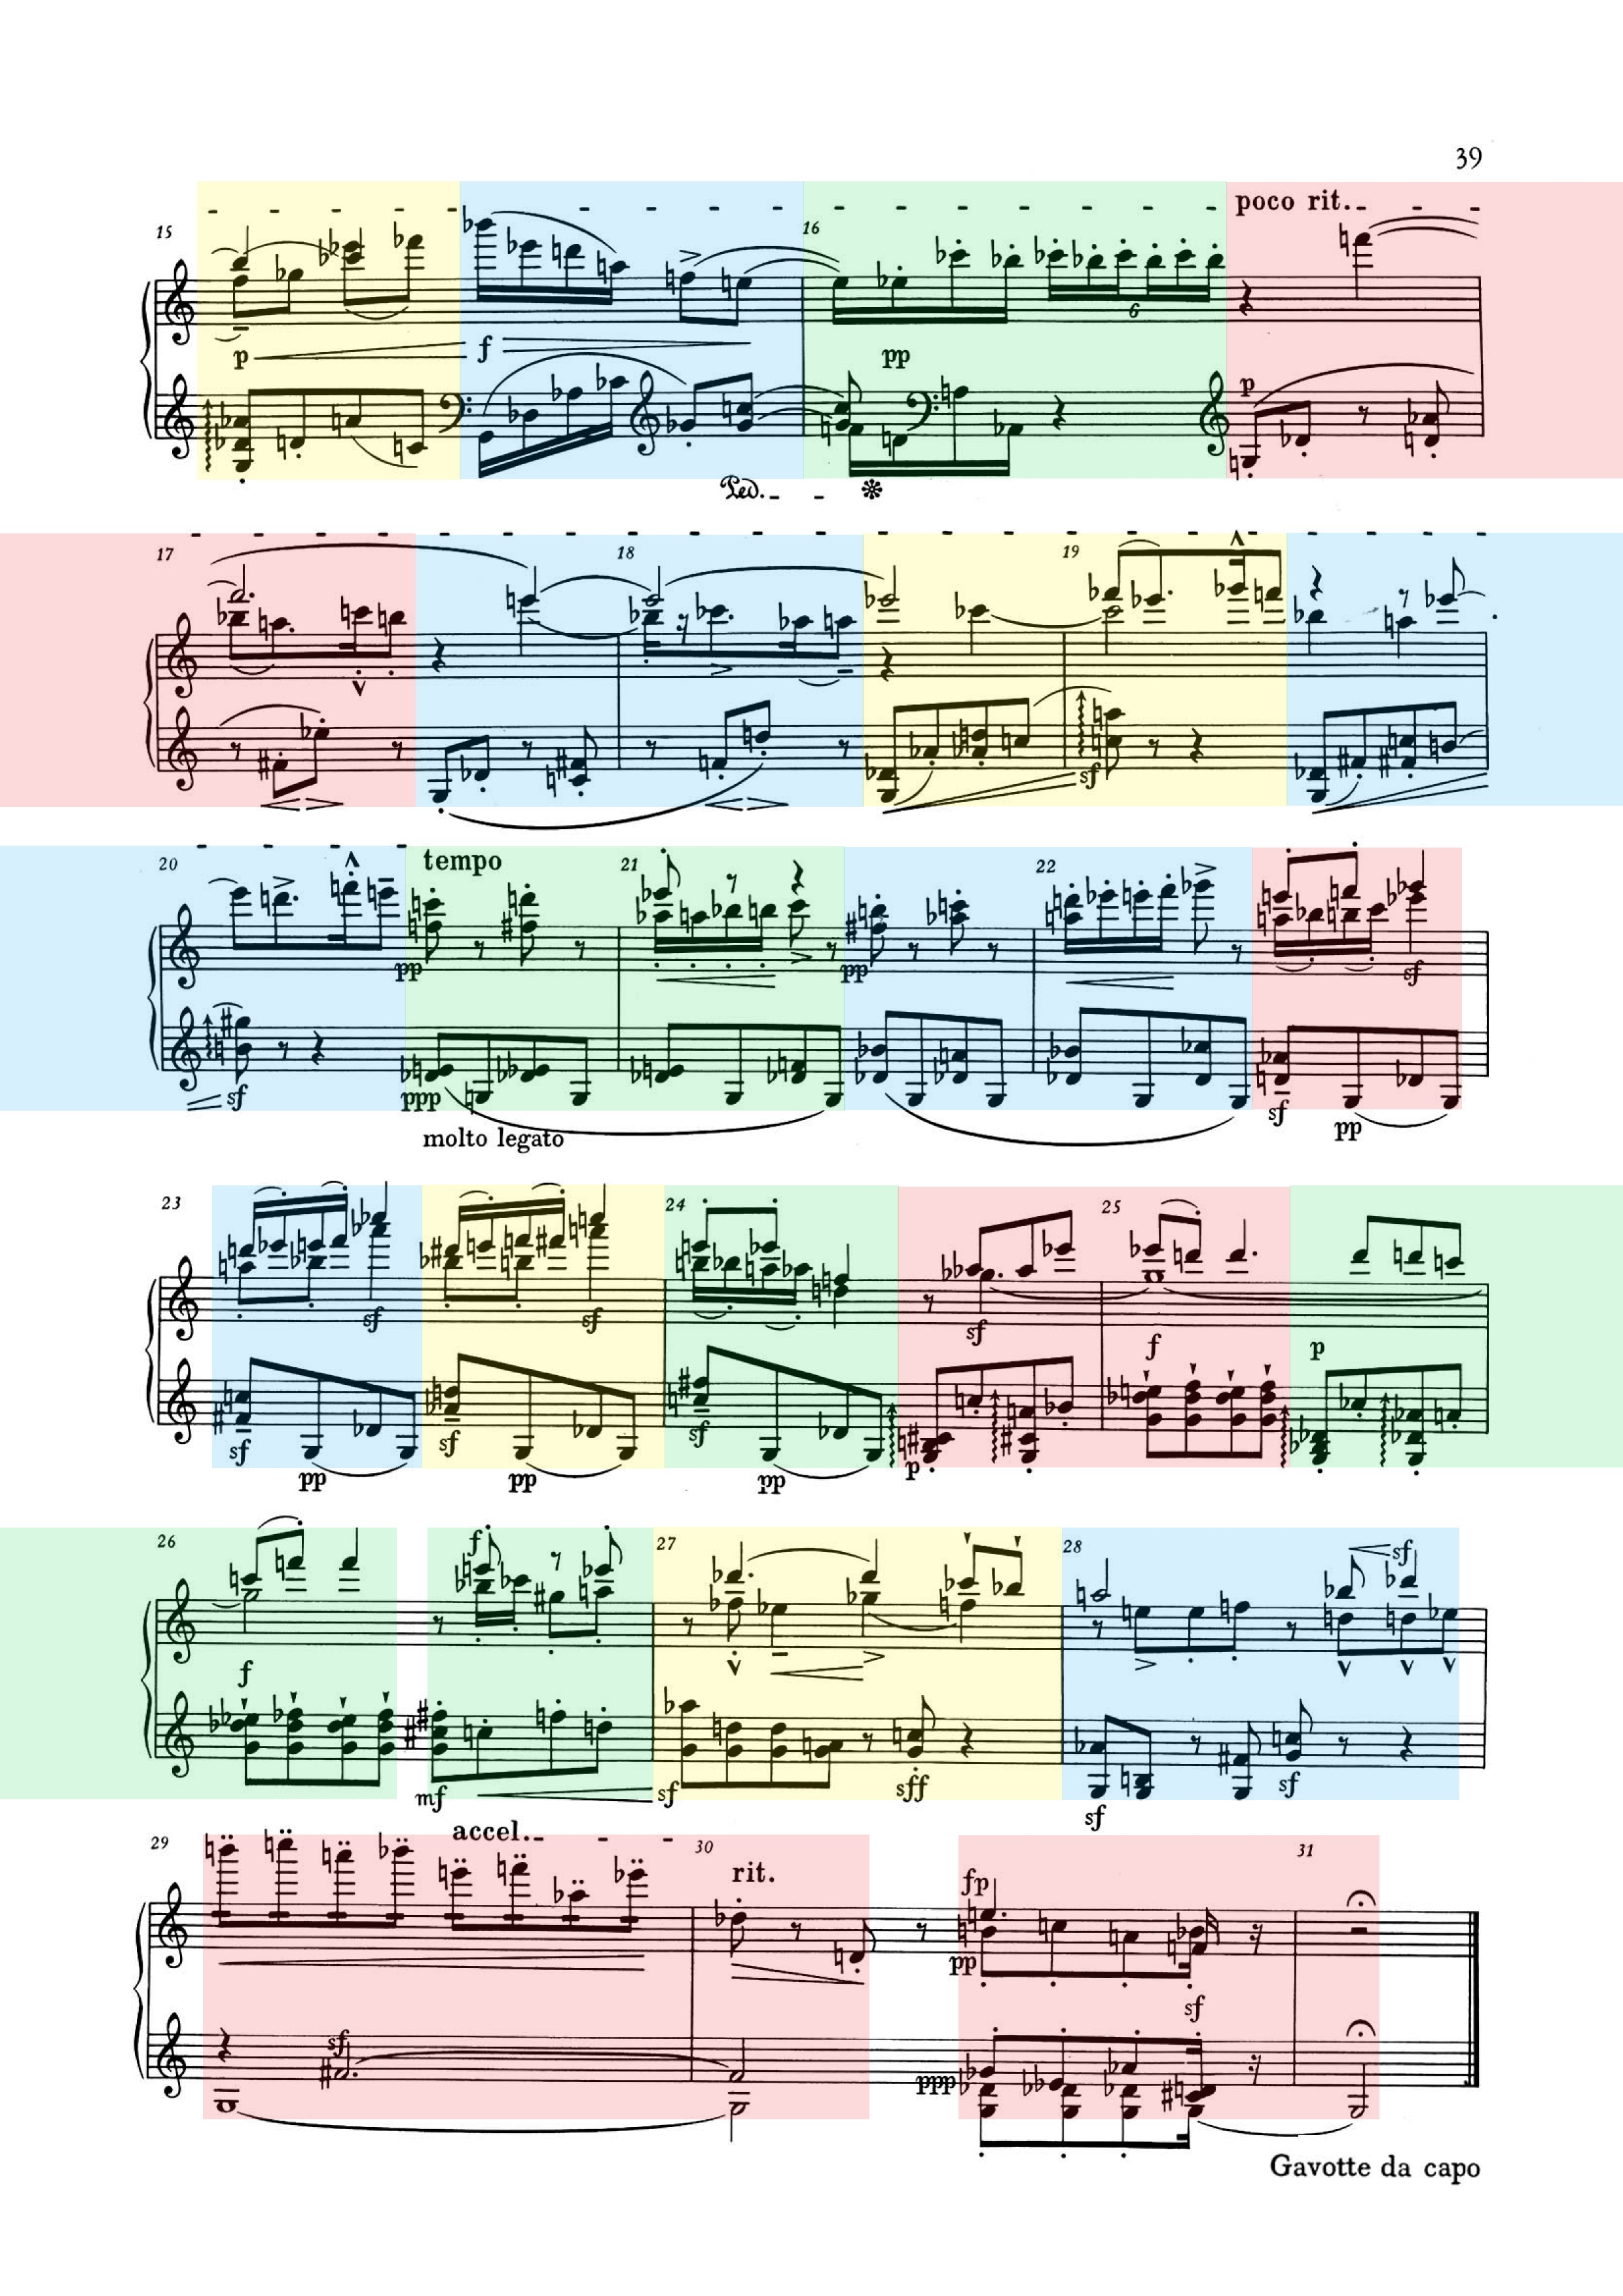
\includegraphics[width=14.5cm]{10.jpg}\\
\caption{An�lisis de la Musette (II)}
\end{center}
\end{figure}		

	\chapter{EL GRUPO DE LAS TRANSFORMACIONES}
	\section{Nuevas definiciones y nuevas transformaciones}
		\label{ciclico}
		Las fórmulas de las transformaciones del apartado \ref{transPsi} quedaron de esta manera:
		\vspace{-0.9cm}
		\begin{multicols}{3}
			$$\text{T}^\text{k}(\sigma(m)) = \sigma(m) + \text{k}$$
			
			$$\text{R}(\sigma(m)) = \sigma(-1-m)$$
			
			$$\text{I}(\sigma(m)) = -\sigma(m) + 2\sigma(0)$$
		\end{multicols} \vspace{-0.3cm}
		
		Sin embargo, la importancia de estas definiciones radica en qué espectro serial forman, y no en cómo se nombra cada serie específica. No es distinguible a un nivel musical y, de hecho, hay más de un convenio para ello.
		
		Han surgido a lo largo de la historia dos métodos para nombrar las series. El primero, el método tradicional, se ha usado desde al menos 1945, y es el método llamado \textit{histórico} en este texto. El segundo, el método de tonos absolutos, fue concebido por George Perle en su libro \emph{Twelve Tone Tonality} (1977).
		
		En el método tradicional, T$_0$ se usa para la primera serie que se encuentra en la composición; es decir, la serie original. En cambio, el método de tonos absolutos nombra las series T basándose solamente en la nota en la que comienzan: T$_0$ se usa para la serie que comienza por un Do, y así sucesivamente. Estas nomenclaturas no caracterizan adecuadamente el objeto matemático que deben representar, es decir, funciones aplicadas a las series. Son nombres arbitrarios que además producen ambigüedad al añadir otras funciones o al intentar describirlo matemáticamente.
		
		En todo caso, cualquier convenio de notación tendrá fórmulas matemáticas distintas al resto, pero todas preservan el material compositivo de la obra. Eso quiere decir que se pueden redefinir algunas de las transformaciones, siempre que preserven el sentido musical. 
		
		Por ejemplo, la inversión puede prescindir de ser transportada para que la primera nota coincida con la original. Para distinguirla de la primera definición, ésta se llamará S de simetría: $\text{S}(\sigma(m)) = -\sigma(m)$.
		
		E igual que la inversión es el cambio de signo por fuera, la retrogradación puede convertirse simplemente en el cambio de signo por dentro. Ésta se llamará V de volteo: $\text{V}(\sigma(m)) = \sigma(-m)$.
		
		Así quedan dos transformaciones que se asemejan a reflexiones: una por \textit{dentro} y otra por \textit{fuera}; y una adición por \textit{fuera}. Aquí \textit{dentro} significa \textit{antes} de aplicar $\sigma$ y \textit{fuera} significa \textit{después} de aplicar $\sigma$, ya que no se debe olvidar que $\sigma$, la permutación, es una función en sí misma. Y ahora surge una cuestión consecuentemente: ¿cuál sería entonces el resultado de sumar \textit{dentro}, es decir, \textit{antes}?
		
		Esta nueva transformación, cuya aparición resulta natural tras las otras tres, se llama \textit{desplazamiento cíclico}. Inventada y usada tan solo por Alban Berg, y en algunas obras primerizas de Schoenberg, C$^\text{k}$ desplaza el comienzo de la serie k posiciones más allá: $\text{C}^\text{k}\left(\sigma\left(m\right)\right)=\sigma\left(m+\text{k}\right)$.
		$$\text{C}^\text{k}=\left(\begin{matrix}0&1&2&&9&10&11\\\sigma\left(\text{k}\right)&\sigma\left(\text{k}+1\right)&\sigma\left(\text{k}+2\right)&\cdots&\sigma\left(\text{k}+9\right)&\sigma\left(\text{k}+10\right)&\sigma\left(\text{k}+11\right)\\\end{matrix}\right)$$
		
		La serie 4-cíclica sobre la permutación P de la Suite Op. 25 es la siguiente serie C$^4$:	
		$$\text{C}^4=\left(\begin{matrix}0&1&2&3&4&5&6&7&8&9&10&11\\6&3&8&2&11&0&9&10&4&5&7&1\\\end{matrix}\right)$$		
		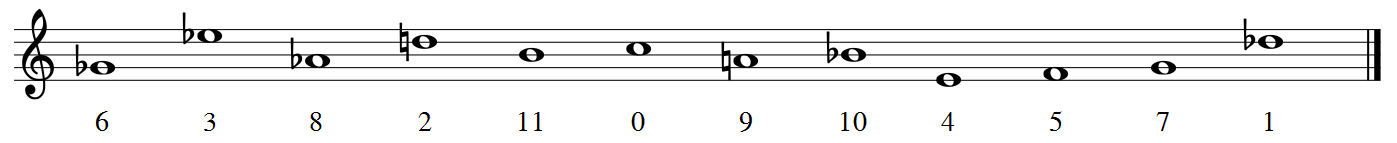
\includegraphics[width=138mm]{13.png}
		
		En resumen, se puede trabajar con un nuevo sistema de definiciones que mantienen el significado musical del serialismo pero varían la notación con la que se trabaja. 
		\vspace{-0.5cm}
		\begin{multicols}{2}
		$$\text{S}(\sigma(m)) = -\sigma(m)$$
		$$\text{T}^\text{k}(\sigma(m)) = \sigma(m) + \text{k}$$
		
		$$\text{V}(\sigma(m)) = \sigma(-m)$$
		$$\text{C}^\text{k}(\sigma(m))=\sigma(m+\text{k})$$
		\end{multicols}
		
		\newpage
	\section{Diagramas de reloj}
	\label{diagramas}
	
		\begin{wrapfigure}{R}{0.23\textwidth}
			\vspace{-0.5cm}
			\begin{tikzpicture}[rotate=30*4,minimum height=0pt,inner sep=0pt,outer sep=0pt,scale=0.75]
			\foreach \x in {0,...,11} {\node at (90-30*\x:2) {\x}; \node (\x) at (90-30*\x:1.6) {};};
			
			\draw [style=flechita] (4)--(5)--(7)--(1)--(6)--(3)--(8)--(2)--(11)--(0)--(9)--(10)--(4);
			
			\node at (0,0) [circle,fill=white] {T$^0$};
			\end{tikzpicture}
			\vspace{-0.5cm}
		\end{wrapfigure}
		Para visualizar mejor cómo actúan las distintas transformaciones, las series se pueden representar mediante \textit{diagramas de reloj}: una sucesión de aristas con una orientación establecida que conecta los vértices de un dodecágono en el orden de la serie. Ya que el desplazamiento cíclico actúa como si la serie fuese circular, hay añadida una arista desde la última nota a la primera. El comienzo de la serie y su orientación se marcan con una flecha.		
		
		A la derecha se incluye el diagrama de la serie original $\sigma$ de la Suite Op. 25. Se pueden distinguir las características de la serie ya comentadas en el apartado \ref{serie25}, como las tres diagonales, que son los tres intervalos de tritono. A continuación se incluyen los diagramas de las transformaciones del apartado \ref{transPsi}: la transposición, la inversión y la retrogradación; así como el nuevo desplazamiento cíclico.
		\begin{multicols}{4}
		\begin{tikzpicture}[scale=0.75,rotate=30*4,minimum height=0pt,inner sep=0pt,outer sep=0pt]
		\foreach \x in {0,...,11} {\node at (90-30*\x:2) {\x}; \node (\x) at (90-30*\x:1.6) {};};
		
		\draw [style=flechita] (5)--(6)--(8)--(2)--(7)--(4)--(9)--(3)--(0)--(1)--(10)--(11)--(5);
		
		\node at (0,0) [circle,fill=white] {T$^1$};
		\end{tikzpicture}		
		\begin{tikzpicture}[scale=0.75,rotate=30*4,minimum height=0pt,inner sep=0pt,outer sep=0pt]
		\foreach \x in {0,...,11} {\node at (90-30*\x:2) {\x}; \node (\x) at (90-30*\x:1.6) {};};
		
		\draw [style=flechita] (4)--(3)--(1)--(7)--(2)--(5)--(0)--(6)--(9)--(8)--(11)--(10)--(4);
		
		\node at (0,0) [circle,fill=white] {I};
		\end{tikzpicture}		
		\begin{tikzpicture}[scale=0.75,rotate=30*4,minimum height=0pt,inner sep=0pt,outer sep=0pt]
		\foreach \x in {0,...,11} {\node at (90-30*\x:2) {\x}; \node (\x) at (90-30*\x:1.6) {};};
		
		\draw [style=flechita] (10)--(9)--(0)--(11)--(2)--(8)--(3)--(6)--(1)--(7)--(5)--(4)--(10);
		
		\node at (0,0) [circle,fill=white] {R};
		\end{tikzpicture}		
		\begin{tikzpicture}[rotate=30*4,minimum height=0pt,inner sep=0pt,outer sep=0pt,scale=0.75]
		\foreach \x in {0,...,11} {\node at (90-30*\x:2) {\x}; \node (\x) at (90-30*\x:1.6) {};};
		
		\draw [style=flechita] (5)--(7)--(1)--(6)--(3)--(8)--(2)--(11)--(0)--(9)--(10)--(4)--(5);
		
		\node at (0,0) [circle,fill=white] {C$^1$};
		\end{tikzpicture}	
		\end{multicols}
		
		La transposición es una rotación en el sentido en el que apunta la flecha; la inversión es una reflexión con el eje de simetría en la diagonal que pasa por la flecha; la retrogradación es un cambio de orientación de la flecha; y el desplazamiento cíclico es el avance interno de la flecha por el recorrido de la serie.
		
		La diferencia entre las inversiones I y S es precisamente la transposición de $2\sigma(0)=8$ semitonos. Comparando S con T$^0$ se puede además observar que S es una reflexión con el eje de simetría en 0, en vez de que el eje dependa de la propia permutación.
		
		\begin{center}
		\begin{multicols}{2}
		\hspace{1.5cm}
		\begin{tikzpicture}[scale=0.75,rotate=30*4,minimum height=0pt,inner sep=0pt,outer sep=0pt]
		\foreach \x in {0,...,11} {\node at (90-30*\x:2) {\x}; \node (\x) at (90-30*\x:1.6) {};};
		
		\draw [style=flechita] (4)--(3)--(1)--(7)--(2)--(5)--(0)--(6)--(9)--(8)--(11)--(10)--(4);
		
		\node at (0,0) [circle,fill=white] {I};
		\end{tikzpicture}
		
		\hspace{-2cm}
		\begin{tikzpicture}[scale=0.75,rotate=30*4,minimum height=0pt,inner sep=0pt,outer sep=0pt]
		\foreach \x in {0,...,11} {\node at (90-30*\x:2) {\x}; \node (\x) at (90-30*\x:1.6) {};};
		
		\draw [style=flechita] (8)--(7)--(5)--(11)--(6)--(9)--(4)--(10)--(1)--(0)--(3)--(2)--(8);
		
		\node at (0,0) [circle,fill=white] {S};
		\end{tikzpicture}
		\end{multicols}
		\end{center}
	
		Por otro lado, la comparación entre las retrogradaciones R y V muestra que, aunque en principio más arbitraria, V es una transformación más natural, ya que deja fija la flecha. La diferencia entre ellas es en realidad un desplazamiento cíclico de -1.
		
		\begin{center}
			\begin{multicols}{2}
				\hspace{1.5cm}
				\begin{tikzpicture}[scale=0.75,rotate=30*4,minimum height=0pt,inner sep=0pt,outer sep=0pt]
				\foreach \x in {0,...,11} {\node at (90-30*\x:2) {\x}; \node (\x) at (90-30*\x:1.6) {};};
				
				\draw [style=flechita] (10)--(9)--(0)--(11)--(2)--(8)--(3)--(6)--(1)--(7)--(5)--(4)--(10);
				
				\node at (0,0) [circle,fill=white] {R};
				\end{tikzpicture}
				
				\hspace{-2cm}
				\begin{tikzpicture}[scale=0.75,rotate=30*4,minimum height=0pt,inner sep=0pt,outer sep=0pt]
				\foreach \x in {0,...,11} {\node at (90-30*\x:2) {\x}; \node (\x) at (90-30*\x:1.6) {};};
				
				\draw [style=flechita] (4)--(10)--(9)--(0)--(11)--(2)--(8)--(3)--(6)--(1)--(7)--(5)--(4);
				
				\node at (0,0) [circle,fill=white] {V};
				\end{tikzpicture}
			\end{multicols}
		\end{center}		
		
	\section[El grupo: D$_{12}$ x D$_{12}$]{El grupo: D$_{\textbf{12}}$ x D$_{\textbf{12}}$}
		\label{grupoD}
		El conjunto de transformaciones \{S, T, V, C\} está compuesto por dos parejas con semejanzas entre sí. S es una reflexión y T una rotación de orden 12 -- es decir, que al aplicarla 12 veces se vuelve a la identidad -- y ambas se aplican a la figura entera; es como mover el diagrama por el papel. En cambio, V es una reflexión de la flecha en sí, y C una rotación -- también de orden 12 -- de la flecha sobre la línea; ambas aplicadas al interior de la figura.
		
		Cada pareja genera un grupo muy conocido: el grupo diédrico o diedral. Se denota por D$_{12}$\footnote{En otros ámbitos, D$_n$ también se denota por D$_{2n}$, ya que $2*n$ es el número de elementos que tiene el grupo.} y representa el grupo de simetrías de un polígono regular; en este caso, un dodecágono. Por ejemplo, aquí se muestran todas las simetrías de un octógono, que son los 16 elementos de D$_{8}$, aplicados a una señal de STOP.
		
		{\scriptsize\begin{tikzpicture}		
		\foreach \i in {0,...,7}
		\node[regular polygon,regular polygon sides=8,draw,rotate=-45*\i] at (1.75*\i,1.75) {STOP};
		\foreach \i in {0,...,7}
		\node[regular polygon,regular polygon sides=8,draw,rotate=-45*\i,xscale=-1] at (1.75*\i,0) {STOP};		
		\end{tikzpicture}}
	
		De igual manera, el conjunto de series de un espectro serial se consigue aplicando a la serie las distintas funciones transformativas; se obtiene entonces un grupo diédrico para ambas parejas de funciones. 
		
		Al haber dos parejas distintas que actúan por separado dentro y fuera de la figura, el grupo completo que forman las cuatro transformaciones es el producto directo de dos copias del diédrico: D$_{12}\times\text{D}_{12}$.
		
		Podemos observarlo claramente si representamos la serie de una segunda forma: como la correspondencia entre vértices de dos dodecágonos. La serie original, que es en realidad una permutación de 12 elementos, se representa como una función: los vértices del dodecágono interno se envían biyectivamente a los vértices externos. Así, $m \longmapsto \sigma(m)$. Este diagrama es similar al matricial pero enroscado en sí mismo, de tal forma que se aprecia la permutación escogida mediante las flechas, que son fijas, y facilita un significado del antes y el después de aplicarla.
		
		Las dos primeras figuras describen esto mismo: la representación de la serie original y la representación de la permutación mediante las flechas, que se mantendrán constantes en el resto de figuras.
		
			
		\begin{multicols}{2}
			\begin{tikzpicture}[minimum height=18pt,inner sep=0]
			\draw foreach \x in {0,...,11} {(90-30*\x:2.5) node[very thin,circle,draw] (\x) {\x}};
			\draw foreach \x in {0,...,11} {(90-30*\x:1.25) node[very thin,circle,draw] {\x}};
			\foreach \y/\x in {0/4,1/5,2/7,3/1,4/6,5/3,6/8,7/2,8/11,9/0,10/9,11/10} {\draw [style=flache] (90-30*\y:1.25) -- (\x);};		
			
			\node at (0,0) [very thin,draw,circle,fill=white] {T$^0$};
			\end{tikzpicture}
			
			\begin{tikzpicture}[minimum height=18pt,inner sep=0]
			\draw foreach \x in {0,...,11} {(90-30*\x:2.5) node (\x) {}};
			\foreach \y/\x in {0/4,1/5,2/7,3/1,4/6,5/3,6/8,7/2,8/11,9/0,10/9,11/10} {\draw [style=flache] (90-30*\y:1.25) -- (\x);};
			
			
			\node at (-3,0) {};
			\end{tikzpicture}
		\end{multicols}
	
		Las cuatro siguientes figuras representan las cuatro funciones transformativas, que son en realidad la reflexión y la rotación del grupo diédrico de cada dodecágono. Aplicarlo al de dentro es aplicarlo antes de las flechas; antes de la permutación. Aplicarlo fuera es transformar después de las flechas; después de la permutación.
			
		\newpage
	
		\begin{multicols}{2}
			\begin{tikzpicture}[minimum height=18pt,inner sep=0]
			\draw foreach \x in {0,...,11} {(90-30*\x:2.5) node[circle] (\x) {}};
			\foreach \y/\x in {0/4,1/5,2/7,3/1,4/6,5/3,6/8,7/2,8/11,9/0,10/9,11/10} {\draw [style=flache] (90-30*\y:1.25) -- (\x);};
			
			\draw foreach \x in {0,...,11} {(90+30*\x:2.5) node[very thin,circle,draw] {\x}};
			\draw foreach \x in {0,...,11} {(90-30*\x:1.25) node[very thin,circle,draw] {\x}};
			
			\draw [red,very thick,dash pattern={on 1pt off 4pt on 10pt off 3pt}] (0,-3.5) -- (0,3.5);
			
			\node at (0,0) [very thin,draw,circle,fill=white] {S};
			\end{tikzpicture}
			
			\begin{tikzpicture}[minimum height=18pt,inner sep=0]
			\draw foreach \x in {0,...,11} {(90-30*\x:2.5) node[circle] (\x) {}};
			\foreach \y/\x in {0/4,1/5,2/7,3/1,4/6,5/3,6/8,7/2,8/11,9/0,10/9,11/10} {\draw [style=flache] (90-30*\y:1.25) -- (\x);};
			
			\draw foreach \x in {0,...,11} {(120-30*\x:2.5) node[very thin,circle,draw] {\x}};
			\draw foreach \x in {0,...,11} {(90-30*\x:1.25) node[very thin,circle,draw] {\x}};
			
			\draw [style=flocho,thick,red,dashed] (90:3) to [bend right=45] (180:3);
			\node at (0,3.25) {};
			
			\node at (0,0) [very thin,draw,circle,fill=white] {T$^1$};
			\end{tikzpicture}
		\end{multicols}
		
		\begin{multicols}{2}
			\begin{tikzpicture}[minimum height=18pt,inner sep=0]
			\draw foreach \x in {0,...,11} {(90-30*\x:2.5) node (\x) [circle] {}};
			\foreach \y/\x in {0/4,1/5,2/7,3/1,4/6,5/3,6/8,7/2,8/11,9/0,10/9,11/10} {\draw [style=flache] (90-30*\y:1.25) -- (\x);};
			
			\draw foreach \x in {0,...,11} {(90-30*\x:2.5) node[very thin,circle,draw] {\x}};
			\draw foreach \x in {0,...,11} {(90+30*\x:1.25) node[very thin,circle,draw] {\x}};
			
			\draw [red,very thick,dash pattern={on 1pt off 3pt on 7pt off 2pt}] (0,-2) -- (0,2);
			
			\node at (0,0) [very thin,draw,circle,fill=white] {V};
			\end{tikzpicture}
			
			\begin{tikzpicture}[minimum height=18pt,inner sep=0]
			\draw foreach \x in {0,...,11} {(90-30*\x:2.5) node[circle] (\x) {}};
			\foreach \y/\x in {0/4,1/5,2/7,3/1,4/6,5/3,6/8,7/2,8/11,9/0,10/9,11/10} {\draw [style=flache] (90-30*\y:1.25) -- (\x);};
			
			\draw foreach \x in {0,...,11} {(90-30*\x:2.5) node[very thin,circle,draw] {\x}};
			\draw foreach \x in {0,...,11} {(60-30*\x:1.25) node[very thin,circle,draw] {\x}};
			
			\draw [style=flocho,thick,red,dashed] (90:1.75) to [bend left=45] (0:1.75);
			
			\node at (0,0) [very thin,draw,circle,fill=white] {C$^1$};
			\end{tikzpicture}
		\end{multicols}
		
		
	\section{Conmutatividad entre los elementos del grupo}
	\label{conmut}
		% comprobar cosos que conmutan, mencionar cosos que conmutan en el otro sistema
		
		La rotación (r) y la reflexión (s) de un grupo diédrico no conmutan, sino que cumplen esta relación: $r\cdot s=s\cdot r^{-1}$. Por otro lado, en los productos directos los elementos de un lado conmutan con los del otro. De esta forma, \{S, T\} no conmutan y \{V, C\} tampoco, pero el resto de parejas de transformaciones deben conmutar. Las verificaciones de estas afirmaciones, que confirman que el grupo formado es D$_{12}\times\text{D}_{12}$, se encuentran en el Anexo \ref{app:commm}, página \pageref{app:commm}.
		
		Volviendo a las definiciones originales, al conjunto de transformaciones \{I, T, R, C\}, la estructura interna es bien distinta. El problema de I, a un nivel matemático, es que depende de la permutación escogida, por lo que a veces tiene unas propiedades y a veces otras. En cambio, la definición de V con respecto a R es meramente estética. Ya que no depende de la permutación, su conmutatividad se mantiene invariante. 
		
		Viendo cómo conmutan los elementos de este sistema se aprecia la dificultad definitoria de I. Curiosamente, la conmutatividad de \{I, R\} e \{I, C\} se pierde, pero se gana la de \{I, T\}. Así, T conmuta con todo en el sistema. Esto refleja que en realidad la motivación de la definición de I viene por esta conmutatividad.
		
		\underline{I y R ya no conmutan:}
		
		$\text{I}\circ\text{R}(\sigma(m))=\text{I}(\text{R}(\sigma(m)))=-\text{R}(\sigma(m))+2\text{R}(\sigma(0))=-\sigma(-1-m)+2\sigma(-1-0)=-\sigma(-1-m)+2\sigma(-1)$
		
		$\text{R}\circ\text{I}(\sigma(m))=\text{R}(\text{I}(\sigma(m)))=\text{R}(-\sigma(m)+2\sigma(0))\overset{\footnote{R y T conmutan}}{=}\text{R}(-\sigma(m))+2\sigma(0)=-\sigma(11-m)+2\sigma(0)$
		
		Los únicos casos en los que podrían conmutar ocurrirían cuando $2\sigma\left(0\right)\equiv2\sigma(11)$ (mod. 12): $12+2\sigma\left(0\right)=2\sigma\left(11\right)\implies\ 6+\sigma\left(0\right)=\sigma\left(11\right)\implies \sigma\left(11\right)-\sigma\left(0\right)=6$. Es decir, cuando la primera y la última nota de la serie original se distancian en 6 semitonos, como es el caso de la permutación en la Suite Op. 25:
		
		$$
		\text{IR}=\text{RI}=\left(\begin{matrix}0&1&2&3&4&5&6&7&8&9&10&11\\10&11&8&9&6&0&5&2&7&1&3&4\\\end{matrix}\right)
		$$	
		
		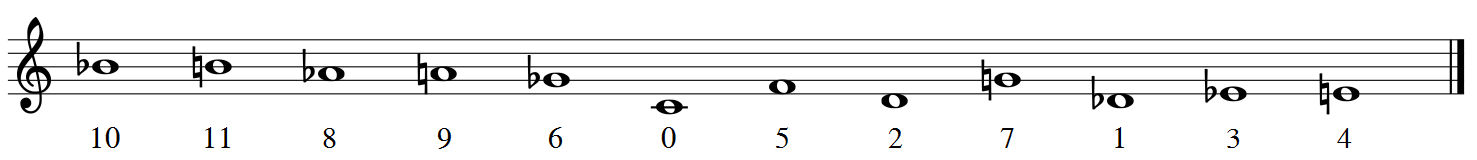
\includegraphics[width=138mm]{5.png}\\
		
		\underline{I y C ya no conmutan:}
		
		$\text{I}\circ\text{C}(\sigma(m))=\text{I}(\sigma(m+1))=-\sigma(m+1)+2\sigma(1)$
		
		$\text{C}\circ\text{I}(\sigma(m))=\text{C}(-\sigma(m)+2\sigma(0))\overset{\footnote{C y T conmutan}}{=}\text{C}(-\sigma(m))+2\sigma(0)=-\sigma(m+1)+2\sigma(0)$
		
		Los únicos casos en los que podrían conmutar ocurrirían cuando $2\sigma\left(0\right)\equiv2\sigma(1)$ (mod. 12): $12+2\sigma\left(0\right)=2\sigma\left(1\right)\implies\ 6+\sigma\left(0\right)=\sigma\left(1\right)\implies \sigma\left(1\right)-\sigma\left(0\right)=6$. Es decir, cuando la primera y la segunda nota de la serie original se distancian en 6 semitonos.
		
		Si se echan las cuentas con C$^\text{k}$ en vez de con C$^1$, pueden conmutar si $\sigma\left(\text{k}\right)-\sigma\left(0\right)=6$. Como $\sigma$ es una permutación, devuelve todos los valores de 0 a 11 y solamente una vez cada uno. Por tanto, también devuelve 6 + $\sigma(0)$, así que siempre existe un único k para el que I y C$^\text{k}$ conmutan. En el caso de la permutación de la Suite Op. 25, como $\sigma\left(0\right)=4$ hay que encontrar el $m$ para el que $\sigma\left(m\right)=4+6=10$. En este caso, $m=11$, pero depende por completo de la permutación original.\\
		
		\underline{I y T ahora sí conmutan:}
		
		$\text{I}\circ\text{T}(\sigma(m))=\text{I}(\sigma(m)+1)=-(\sigma(m)+1) + 2(\sigma(0)+1)=-\sigma(m)-1+2\sigma(0)+2=-\sigma(m)+2\sigma(0)+1$
		
		$\text{T}\circ\text{I}(\sigma(m))=\text{T}(-\sigma(m)+2\sigma(0))=-\sigma(m)+2\sigma(0)+1$\\
		
		\underline{R y C no conmutan:}
		
		$\text{R}\circ\text{C}(\sigma(m))=\text{R}(\sigma(m+1))=\sigma(-(m+1)-1)=\sigma(-m-2)$
		
		$\text{C}\circ\text{R}(\sigma(m))=\text{C}(\sigma(-m-1))=\sigma(-m-1+1)=\sigma(-m)$\\
		
		\underline{T y R conmutan:}
		
		$\text{T}\circ\text{R}(\sigma(m))=\text{T}(\sigma(-m-1))=\sigma(-m-1)+1$
		
		$\text{R}\circ\text{T}(\sigma(m))=\text{R}(\sigma(m)+1)=\sigma(-m-1)+1$\\
		
		\underline{T y C conmutan:}
		
		$\text{T}\circ\text{C}(\sigma(m))=\text{T}(\sigma(m+1))=\sigma(m+1)+1$
		
		$\text{C}\circ\text{T}(\sigma(m))=\text{V}(\sigma(m)+1)=\sigma(m+1)+1$

	\newpage$\ $
	\thispagestyle{empty}
	\cleardoublepage
    
	\part{ENEFONISMO}
	\chapter{EL SURGIMIENTO DEL SERIALISMO INTEGRAL}
	\section{Alban Berg y Anton Webern: la Segunda Escuela de Viena}
	\label{berweb}
	Además de Schoenberg, hubo dos compositores más que contribuyeron al desarrollo del dodecafonismo y que demostraron con sus diferentes estilos la versatilidad del sistema. Éstos fueron los discípulos de Schoenberg: Alban Berg y Anton Webern. 
	
	El maestro y sus dos alumnos formaron la autodenominada Segunda Escuela de Viena, llamada así en honor a los miembros de la Primera Escuela de Viena: Haydn, Mozart y Beethoven. Aparte del hecho de que Schoenberg, Berg y Webern nacieron y se formaron en Viena, el nombre también simboliza su autoproclamación como herederos legítimos de la tradición musical alemana proveniente del siglo XVIII.
	
	La Segunda Escuela de Viena formó parte de las vanguardias artísticas europeas, opuestas a la tendencia neoclásica de Stravinsky o Prokofiev. Los tres integrantes siguieron carreras compositivas similares en cuanto a estilo y concepción artística: una época tonal, una ruptura atonal y un desarrollo dodecafónico.
	
	Con el ascenso del nazismo, Schoenberg, que era judío, se vio obligado a exiliarse a Estados Unidos. Sus discípulos se quedaron en Austria, pero pasaron penurias económicas debido a la censura impuesta por el gobierno: la música dodecafónica se descalificó como \emph{Entartete Musik} (<<música degenerada>>).
	
	\begin{wrapfigure}{L}{0.3\textwidth}
		\captionsetup{justification=centering, font=footnotesize}
		\vspace{-\bigskipamount}
		\centering{
			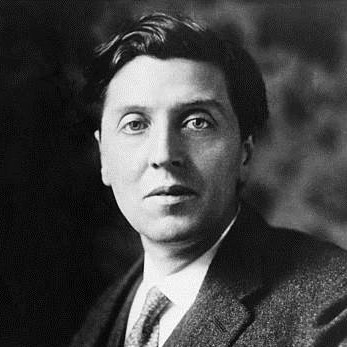
\includegraphics[width=0.22\textwidth]{Alban_Berg.jpg}			
			\caption*{Alban Berg\\(1885--1935)}	}
	\end{wrapfigure}
	Alban Berg se centró en la efusión emocional y el interés por lo humano, utilizando el método dodecafónico libremente y acercándose a formatos tonales. Su etapa atonal fue especialmente relevante, ya que compuso entonces su primera obra dramática, Wozzeck (1925). Es una ópera basada en la pieza teatral de Georg Büchner, en la cual Berg plasmó parte de sus propias experiencias como soldado en la Primera Guerra Mundial. Su segunda ópera, Lulú, quedó inconclusa debido a su muerte por septicemia en 1935, a los 50 años.
	
	Anton Webern fue un compositor más riguroso en cuanto a las formas, siempre leal al sistema dodecafónico y a su maestro. Se deleitaba en los procedimientos formales más sutiles, aquellos que solo podían ser descubiertos al estudiar detenidamente la obra. Esto quedó reflejado en su dodecafónico Concierto para 9 instrumentos, Op. 24 (1934), cuya serie está construida por segmentos derivados de las tres primeras notas de la obra. Además, muestra tendencias a asignar duraciones, timbres y articulaciones a segmentos aislados, lo que más tarde inspiraría el serialismo integral.
        
	Durante la ocupación de Viena, Webern salió de su casa una noche tras el toque de queda, y un soldado norteamericano, probablemente en estado de embriaguez, lo mató a tiros. Así, Schoenberg, el maestro y el más mayor de los tres, sobrevivió a sus dos alumnos exiliado en Estados Unidos.
    
	\section{La escuela de Darmstadt}
	Tras la Segunda Guerra Mundial, el mundo artístico estaba totalmente destruido. La violencia, la censura y la incomunicación habían impedido cualquier posible desarrollo creativo, y los artistas de la generación anterior se habían aislado, exiliado o habían fallecido. Volver a construir los pilares del arte era el cometido de la nueva generación de artistas, quienes compartían la sensación de que el mundo había renacido y el tiempo había comenzado de nuevo.
	
	En 1946 se fundaron los Cursos de Verano de Darmstadt, fundados por Wolfgang Steinecke y patrocinados por las fuerzas americanas, con el objetivo de retomar la actividad musical en la Alemania de la posguerra. Los cursos se centraron en dar a conocer las técnicas compositivas de las generaciones anteriores. Aunque el primer año estuvo enfocado en el movimiento neoclásico, fue en los años posteriores cuando se desarrolló un mayor interés por las técnicas serialistas.
	
	Los cursos resultaron en la aparición de una nueva escuela de compositores cuya finalidad artística era crear un lenguaje musical distinto y alejado de la tradición para, de esta forma, obtener una mayor libertad compositiva. Como dijo Karlheinz Stockhausen:
	
	\begin{quote}
%		\textit{New methods change the experience, and new experiences change man. Whenever we hear sounds, we are changed, we are no longer the same, and this is more the case when we hear organized sounds; music.}
		\textit{Los métodos nuevos cambian la experiencia, y las experiencias nuevas cambian al hombre.}\footnote{Karlheinz Stockhausen en el documental autobiográfico \textit{Tuning In} (1981).}
	\end{quote}
	
	Esta escuela tomó el nombre de la ciudad donde se realizaban los cursos: se llamó la Escuela de Darmstadt. El término fue acuñado por el compositor Luigi Nono en una de sus clases magistrales en 1957, y con él se describía a sí mismo y a sus compañeros compositores: Pierre Boulez, Karlheinz Stockhausen y Bruno Maderna. Para estos compositores, la tradición artística estaba demasiado relacionada con los fracasos políticos y las penurias sociales pasadas, y precisamente por ello creían necesario romper con todos los vínculos heredados.
	
	\pagebreak
	
	\begin{wrapfigure}{R}{0.3\textwidth}
		\captionsetup{justification=centering, font=footnotesize}
		\centering{
			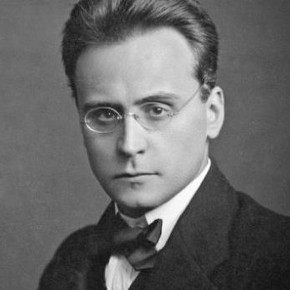
\includegraphics[width=0.22\textwidth]{Anton_Webern.jpg}			
			\caption*{Anton Webern\\(1883--1945)}	}
	\end{wrapfigure}
    Sin embargo, para crear aquel nuevo lenguaje no tomaron como referencia el dodecafonismo de Schoenberg, ya que él veía su sistema como parte de la tradición musical, como un elemento más en la evolución de la música. Se centraron, en cambio, en la formalidad y abstracción del serialismo de Anton Webern, y desarrollaron a partir de sus métodos el denominado \emph{serialismo integral}.
    
    Para la Escuela de Viena, el estilo compositivo de Webern era tan solo un posible enfoque del amplio abanico que abarcaba el dodecafonismo, pero la Escuela de Darmstadt lo consideró como un avance de éste.
	
	El serialismo integral es un sistema de composición musical que predetermina los materiales compositivos -- la melodía, la armonía, el ritmo, el timbre -- a partir de la ordenación serial de los diferentes parámetros musicales: alturas, intensidades, duraciones, ataques o instrumentos, entre otros. 
	
	Es un desarrollo del serialismo dodecafónico de Schoenberg, que serializa solamente las alturas, hacia los demás parámetros sonoros. Tiene, por tanto, un alto grado de planificación pre-composicional: se pretende que la determinación compositiva sea absoluta; y se tiende al automatismo del arte y sus formas, alejándolo de cualquier evocación decimonónica.

	Desde sus comienzos, el serialismo integral suscitó numerosas críticas, incluso desde el propio colectivo vanguardista. Una de ellas fue la falta de elección del intérprete a la hora de transmitir la obra. El intérprete serialista debe reproducir con total exactitud cada detalle de la partitura, y, por tanto, no puede aportar carácter alguno. 
	
	Otra de las críticas más extendidas fue la incapacidad para interpretar estas obras correctamente debido a su complejidad técnica. Además, los detalles que precisamente las hacen complejas son, en su mayor parte, inapreciables por parte del oyente.
	
	\pagebreak
	
	\section{Pierre Boulez}
	\label{boulez}
     \begin{wrapfigure}{L}{0.3\textwidth}
		\captionsetup{justification=centering, font=footnotesize}
		\vspace*{-\bigskipamount}
		\centering{
			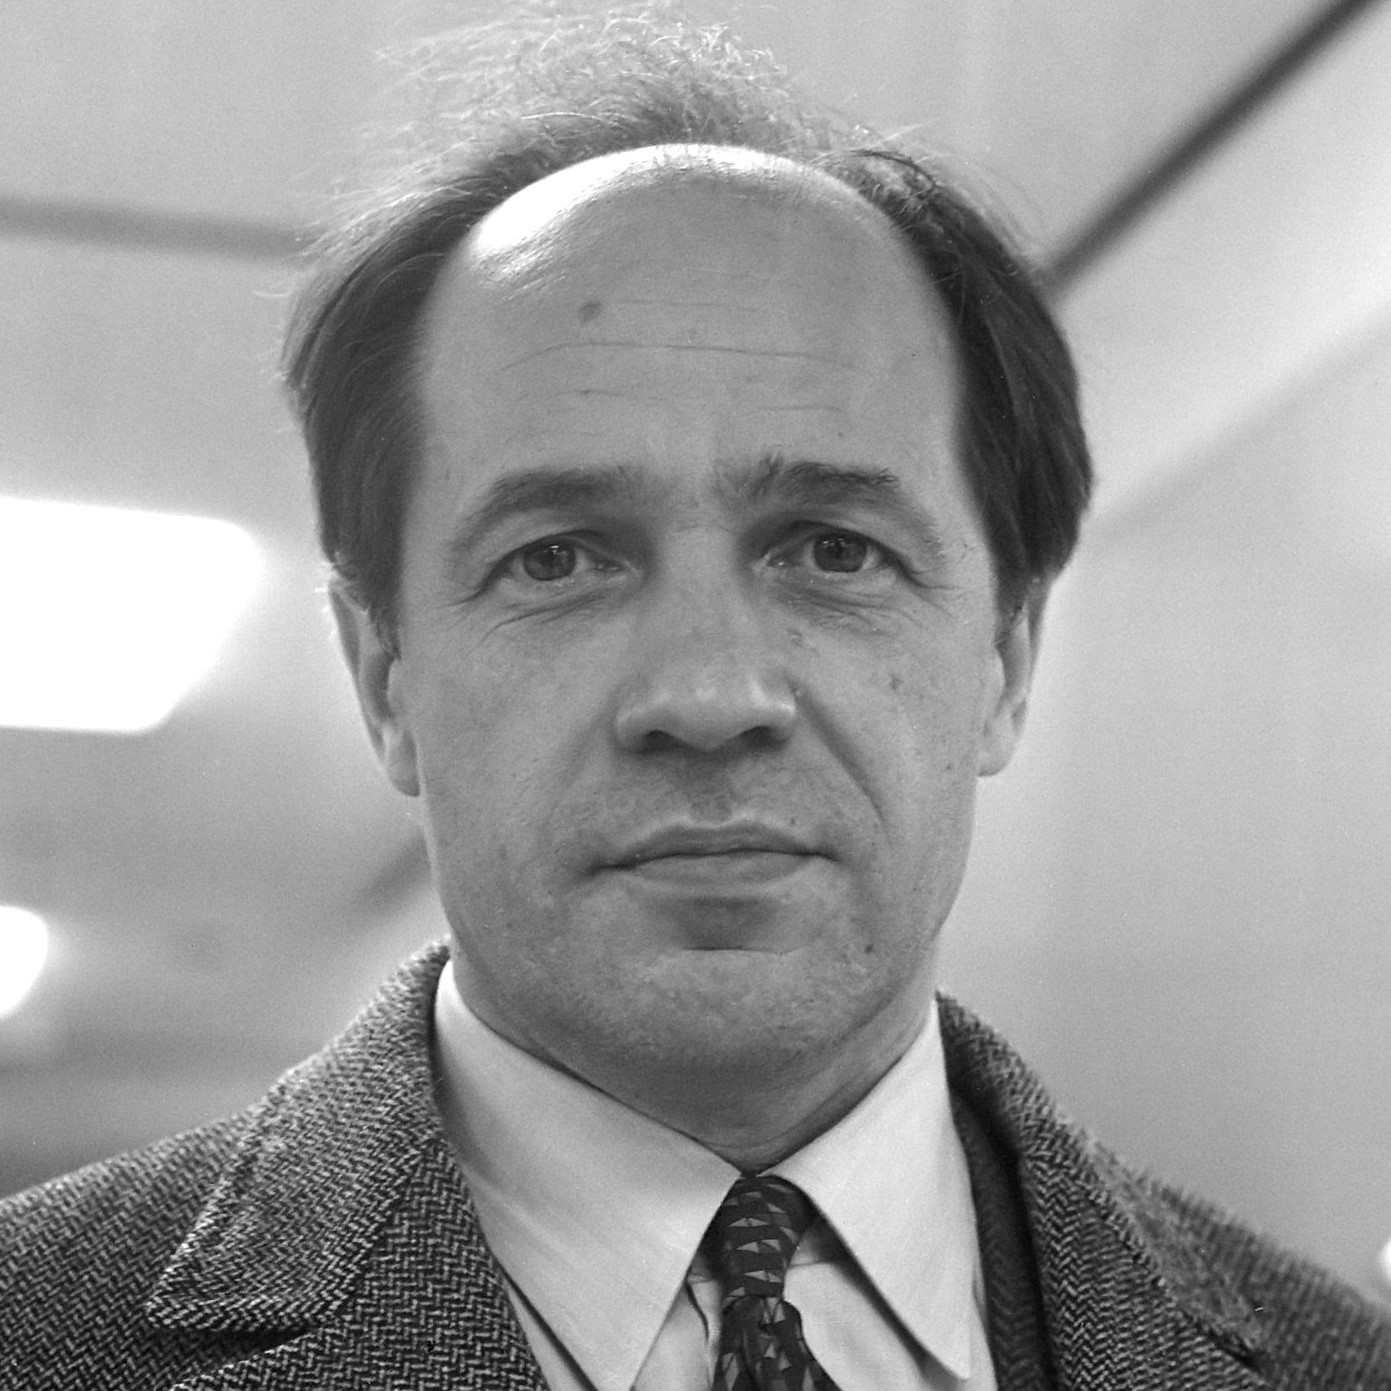
\includegraphics[width=0.22\textwidth]{Pierre_Boulez.jpg}			
			\caption*{Pierre Boulez\\(1925--2016)}	}
	\end{wrapfigure}
    El compositor que creó y utilizó por primera vez el serialismo integral, además de instruirlo y difundirlo a los demás compositores de Darmstadt, fue el compositor francés Pierre Boulez. Otros músicos habían compuesto obras con tendencias serialistas y elementos predeterminados, como Olivier Messiaen en \emph{Mode de valeurs et d’intensités}, pero fue Boulez quien sentó sus bases y su técnica. De hecho, los compositores precedentes influyeron prominentemente en la música de Boulez gracias a las clases impartidas en los cursos de Darmstadt.
    
    Boulez consideraba necesaria y evidente la extensión de elementos a predeterminar más allá de la melodía, y le parecía incoherente el sistema dodecafónico de Schoenberg, que para él estaba incompleto. En su controvertido ensayo \emph{Schoenberg ha muerto}, publicado un año después de la muerte del compositor, comentó:
    
    \begin{quote}\emph{En primer lugar, la exploración del campo serial ha sido conducida unilateralmente: allí falta el plano rítmico, e incluso el plano sonoro propiamente dicho: las intensidades y los ataques.} [$\ldots$] 
    	
    \emph{Pero la causa esencial de su fracaso reside en el desconocimiento profundo de las FUNCIONES seriales propiamente dichas, las funciones engendradas por el principio mismo de la serie.} \cite{boulez}\end{quote}
    
   Es decir, que para ampliar el concepto de serialismo se debía primeramente conocer el fundamento matemático de las series y sus funciones transformativas. Además de ser músico y compositor, Boulez había estudiado matemáticas, lo que le llevó a querer analizar matemáticamente el sistema compositivo y generalizarlo para series de longitudes arbitrarias. Para él, el serialismo no debía ser un mero recurso compositivo, sino la ley que rige todos los elementos de la obra. De hecho, más adelante en su ensayo declara:
    
    \begin{quote}[\ldots] \emph{desde el descubrimiento de la Escuela de Viena, todo compositor alejado de los experimentos seriales ha resultado inútil.}\end{quote}

	Su obra \emph{Structures I} (1952), para dos pianos, fue compuesta siguiendo las técnicas de serialismo integral: tiene series de doce alturas, doce ataques, doce duraciones y
doce tipos dinámicos, aunque más tarde reduciría algunas a diez.
	\chapter{MÁS HERRAMIENTAS MATEMÁTICAS}\label{ch:acciones}
	\section{Acciones de grupos sobre conjuntos}
		Dado un grupo (G, $*$) y un conjunto X, la \emph{acción} de (G, $*$) sobre X es una función $\phi$ que asocia un elemento $g \in$ G y un elemento $x \in$ X -- el par ($g$, $x$) -- a otro elemento $g\cdot x$ que también pertenece a X \cite{armstrong}. $\ \ \phi :(g,x) \to g\cdot x$
	
		La acción $\phi$, expresada mediante la operación ($\cdot$), debe cumplir dos condiciones:
		\begin{enumerate}
			\item{Para todo $x\in$ X, $e\cdot x=x$, siendo $e$ el elemento neutro del grupo.}
		
			\item{Para todo $x\in$ X y para todo par $g,h\in$ G, se debe cumplir que $(g*h)\cdot x=g\cdot (h\cdot x)$. La primera operación ($*$) es la interna del grupo G, y la segunda operación ($\cdot$) es la acción.}
		\end{enumerate}
		Como ya se ha visto en el apartado \ref{grupoD}, las funciones \{S,T,V,C\} forman el grupo diédrico $\text{D}_{n}\times\text{D}_{n}$, con $n$ la longitud de la serie. Se podrá definir entonces la acción $\phi$ de este grupo sobre el conjunto de permutaciones de orden $n$, tal que $\phi(\Psi,\ \sigma)=\Psi\circ\sigma=\Psi(\sigma)=\tau$, con $\Psi\in\text{D}_{n}\times\text{D}_{n}$ y $\sigma,\tau\in\text{S}_n$.
		
		De igual manera, se puede definir el grupo que forman solamente I y R, que servirá más adelante. Como son dos reflexiones, forman el conocido grupo de Klein -- a partir de ahora denotado por $\Xi$, con elementos Id, I, R e IR.

	\section{Órbitas y estabilizadores}	
		Dada una acción de (G, $*$) sobre X, la \emph{órbita} de un determinado elemento $x_0\in$ X es el subconjunto de elementos $x$ de X que pueden ser alcanzados desde $x_0$ mediante algún $g_0\in$ G. Es decir, todos los $x$ para los que existe un $g_0$ que al actuar sobre $x_0$ da $x$. Trivialmente, $x_0\in Orb(x_0)$ ya que $e\cdot x_0=x_0$.
		\[Orb(x_0)=\{x\in X :\ \exists \ g_0\in \text{G},\ g_0\cdot x_0 =x\}\]
	
		Por ejemplo, dada una permutación $\sigma$, todas las permutaciones a las que se llega desde $\sigma$ mediante algún $\Psi\in\text{D}_{n}\times\text{D}_{n}$ -- que son las transformaciones de series del apartado \ref{ciclico} -- conforman la órbita de $\sigma$. Por definición, las series a las que se puede llegar desde una serie original conforman su espectro serial, por lo que \textbf{la órbita es en realidad el espectro serial}.
	
		Para el mismo $x_0$ se define su \emph{estabilizador} como el conjunto de elementos $g\in$ G que fijan $x_0$, es decir, que mandan $x_0$ a sí mismo. Mientras que una órbita es un subconjunto de X, un estabilizador es un subgrupo de G. Trivialmente, $e\in Stab(x) \ \forall x\in$ X, porque el elemento identidad fija cualquier otro elemento por definición.
		\[Stab(x_0)=\{g\in \text{G}\ :\ g\cdot x_0 =x_0 \}\]
	
		Si cada $g\in$ G llevara a $x_0$ a un $x$ distinto, el número de elementos de $Orb(x_0)$ sería igual al número de elementos de G. Sin embargo, si un elemento $g_0\in$ G fija $x_0$, entonces no dará nuevos elementos en la órbita de $x$. Por tanto, el tamaño de la órbita disminuye. De hecho,  el teorema de Órbita--Estabilizador dice que el tamaño de una órbita ($|Orb(x_0)|$) será el tamaño de G ($|$G$|$) entre el número de elementos que fijan $x_0$; es decir, el tamaño de su estabilizador ($|Stab(x_0)|$). Además, es cierto para todo $x\in$ X.
		\[|Orb(x)|=\frac{|\text{G}|}{|Stab(x)|}\text{, o lo que es lo mismo, }|\text{G}|=|Orb(x)||Stab(x)|\]
		
		\def\arraystretch{1.5}
		Este teorema implica que los tamaños de cada órbita y cada estabilizador son divisores del tamaño del grupo. Por ejemplo, como el tamaño del grupo $\Xi$ es 4, cualquier estabilizador y cualquier órbita tendrán tamaño 1, 2 o 4. En concreto, como Id está siempre en el estabilizador, para  todo $\sigma$ será de una de estas formas:
		\[\begin{matrix}|Stab|=1&&&\{\text{Id}\}&\\\hline|Stab|=2&&\{\text{Id, R}\}&\{\text{Id, I}\}&\{\text{Id, RI}\}\}\\\hline|Stab|=4&&&\{\text{Id, R, I, RI}\}&\\\end{matrix}\]
		
		\def\arraystretch{1}
		Una serie $\sigma$ sin simetrías tendrá una serie distinta para cada una de sus transformaciones. Por tanto, su órbita será \{$\sigma$, R($\sigma$), I($\sigma$), RI($\sigma$)\} y su estabilizador será solamente \{Id\}. Cumple entonces el teorema: $4\cdot 1 = 4$.
	
	\section{El lema de Burnside}
		\label{burnside}
		Las órbitas, que son subconjuntos de X, forman una \emph{partición} de X. Esto significa que son subconjuntos disjuntos: ningún $x$ puede estar en dos órbitas distintas. Interesa entonces saber cuántos subconjuntos hay; es decir, el número de órbitas ($\#Orb$). El lema de Burnside\footnote{Aunque Burnside demostró este lema en una ocasión, citó a Frobenius como su autor. Sin embargo, Cauchy era conocedor del lema décadas antes. Para no confundirlo con otros lemas que sí son de Burnside, a veces se le llama \emph{el lema que no es de Burnside.}} afirma que se pueden calcular así:
		\[\#Orb=\frac{1}{|\text{G}|}\sum_{x\in\text{X}}|\text{Stab}(x)|\]	
		Se prueba de esta forma: por el teorema de Órbita--Estabilizador, $|\text{Stab}(x)|=\frac{|\text{G}|}{|Orb(x)|}$, por lo que la parte derecha se puede expresar así:
		\[\frac{1}{|\text{G}|}\sum_{x\in\text{X}}|\text{Stab}(x)|=
		\frac{1}{|\text{G}|}\sum_{x\in\text{X}}\frac{|\text{G}|}{|Orb(x)|}=
		\sum_{x\in\text{X}}\frac{1}{|Orb(x)|}\]

		Como las órbitas forman una partición de X, la suma sobre todo el conjunto X puede ser dividida en sumas separadas para cada órbita. Además, si por cada elemento de una órbita se suma el inverso del número de elementos de la órbita, esa suma dará uno. Solo queda ahora sumar uno por cada órbita.
		\[\sum_{x\in\text{X}}\frac{1}{|Orb(x)|}=\sum_{\text{O}\in\text{Órbitas}}\left(\sum_{x\in\text{O}}\frac{1}{|\text{O}|}\right)=\sum_{\text{O}\in\text{Órbitas}}1=\#Orb \qed\]	
	
		Este lema permite calcular el número de posibles espectros seriales distintos, ya que el espectro de una serie es igual al espectro de sus series transformadas. Un compositor serialista debe entonces escoger no una serie original, sino el espectro con el que construir la obra. O, más bien, si escoge una serie original está escogiendo el mismo material que si escogiera otra serie de ese mismo espectro.
    \section{Conteo de espectros seriales}\label{ch:espectros}
	\subsection{Espectros de las funciones $\{I,\ T,\ R\}$}
		\label{s:itr}
		Es interesante conocer el n�mero de espectros seriales distintos que un compositor puede escoger. Al fin y al cabo, es irrelevante qu� serie se escoge como la original dentro de su espectro serial, ya que produce el mismo material compositivo que cualquiera de su mismo espectro.
		
		Para calcular el n�mero de espectros seriales se redefinir�n las funciones transformativas para una longitud serial arbitraria, $n$, que ser� mayor que 2. Para $n=0,\ 1$ y 2 se realizar� el c�lculo en el apartado \ref{s:trivcase}.
	
		Adem�s, como las transposiciones siempre son distintas entre s�, siempre pertenecen al mismo espectro. Se tomar�n a partir de ahora todas ellas como equivalentes, de manera que solo se necesita hacer el c�lculo para $\{I,\ R\}$.
		
		Al calcular con permutaciones se trabajar� m�dulo $n$. La retrogradaci�n sigue siendo $R(\sigma(m))=\sigma(-1-m)$. La inversi�n ser� $I(\sigma(m))=-\sigma(m)$, omitiendo la transposici�n habitual, ya que se toman las series transpuestas como equivalentes. De esta forma $-\sigma(m)+2\sigma(0)\equiv-\sigma(m)$. La retrogradaci�n invertida es, por tanto, la composici�n de ambas: $RI(\sigma(m))={I}\circ{R}(\sigma(m))={I}\left({R}(\sigma(m))\right)=-\sigma(-1-m)$.			
		
		La retrogradaci�n, la inversi�n y la composici�n de ambas cumplen que al aplicarlas dos veces se vuelve a la serie original. En teor�a de grupos se dice que tienen \textit{orden 2}. Entonces $\{Id,\ I,\ R,\ IR\}$ forma el ya mencionado grupo de Klein ($\Xi$), donde $RI$ $\equiv$ $IR$, ya que estamos tomando las series transpuestas como equivalentes. 
		
		En general, un grupo de Klein es el formado por cuatro elementos donde cada elemento es inverso de s� mismo. El grupo de Klein, llamado as� en honor al matem�tico alem�n Felix Klein, es el grupo $\mathbb{Z}/(2)\times\mathbb{Z}/(2)$, producto directo de dos grupos c�clicos de orden 2.
		
		Por el lema de Burnside:
		\[\#\mbox{Espectros}=\frac{1}{|\mathbb{Z}/(2)\times\mathbb{Z}/(2)|}\sum_{\sigma\in{S}_n}|{Stab}(\sigma)|=\frac{1}{4}\sum_{\sigma\in{S}_n}|{Stab}(\sigma)|\]
		
		Es decir, se deben calcular para cada posible serie $\sigma\in{S}_n$ cu�ntas funciones transformativas lo dejan igual o equivalente bajo transposici�n.
		
		Como los estabilizadores son subgrupos, por el teorema de Lagrange su tama�o debe ser divisor del tama�o del grupo total. Entonces se pueden agrupar los estabilizadores por sus tama�os: 1, 2 o 4, y as� calcular $\sum|{Stab}(\sigma)|$ agrupando todas las permutaciones con igual tama�o de estabilizador. Si $\#\sigma_i$ es el n�mero de permutaciones cuyos estabilizadores tienen tama�o $i$:		
		\[\sum_{\sigma\in{S}_n}|{Stab}(\sigma)|=1\cdot(\#\sigma_1)+2\cdot(\#\sigma_2)+4\cdot(\#\sigma_4)\]
	
		Primero, se ha de ver que una permutaci�n nunca va a ser igual ni equivalente mediante transposiciones a su inversa.

%		\begin{align*}
%		-\sigma(m)&\equiv\sigma(m)\Longleftrightarrow\\
%		0&\equiv2\sigma(m)\Longleftrightarrow\\
%		n&\equiv2\sigma(m)\Longleftrightarrow\\
%		\frac{n}{2}&\equiv\sigma(m)
%		\end{align*}
\begin{center}
		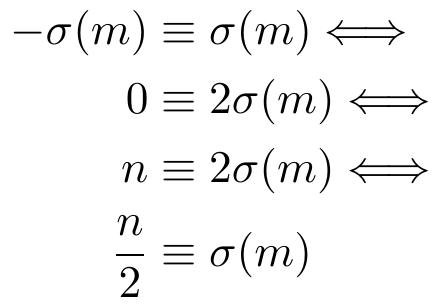
\includegraphics{Serialismo-matematicas-diagrama-2}
\end{center}
		
		As�, $\sigma(m)$ ser�a constante para todo $m\in \mathbb{Z} / (n)$, lo cual es imposible. Esto implica que ninguna permutaci�n va a tener a $I$ en su estabilizador, por lo que $\#\sigma_4=0$. Queda entonces calcular cu�ntas permutaciones son equivalentes a su retrogradaci�n y cu�ntas a su retrogradaci�n inversa. La suma de ambas dar� $\#\sigma_2$.
	
	\subsubsection[Elementos estables mediante $R$]{Elementos estables mediante ${R}$}
		Las permutaciones que coinciden con alguna transposici�n de su retrogradaci�n cumplen, para $\gamma$ constante:
		
		\hspace*{8.5\bigskipamount} $\gamma+\sigma(m) = {R}(m) = \sigma(-1-m)$
		
		Aplic�ndolo a $(-1-m)$:
		$\gamma+\sigma(-1-m) = \sigma(m)$
		
		De ambas ecuaciones: $\quad\gamma=\sigma(-1-m)-\sigma(m)=\sigma(m)-\sigma(-1-m)$
		
		$2\sigma(m)\equiv2\sigma(-1-m)\implies2\sigma(m)-2\sigma(-1-m)\equiv0$
		
		$2\sigma(m)-2\sigma(-1-m)=n \implies \sigma(m)-\sigma(-1-m)=\frac{n}{2}$
		
		Entonces $n$ debe ser par. Cuando $n$ es impar este tipo de permutaciones no existe. Adem�s, cumplen que sus elementos sim�tricos se distancian entre s� un intervalo de $\frac{n}{2}$ unidades: son series con simetr�a par.
		\[\gamma=\sigma(m)-\sigma(-1-m)=\frac{n}{2}\]
		
		En una serie de longitud $n$, existen $\frac{n}{2}$ intervalos que miden $\frac{n}{2}$. Como no importa por cu�l de ellos comience la serie, ya que las transportaciones son equivalentes, se fija el primero de los intervalos. Quedan los otros $\frac{n}{2}-1$ intervalos por escoger, as� que el n�mero de series con simetr�a par cuenta las permutaciones de $\frac{n}{2}-1$ intervalos y las dos posibles posiciones de cada intervalo \textemdash creciente y decreciente~\cite{reiner}\textemdash. Por ello, el n�mero de series con simetr�a par es de:
		
		\[2! \cdot \left(\frac{n}{2}-1\right)! = 2\left(\frac{n-2}{2}\right)!=(n-2)(n-4)\ldots=(n-2)!!\]
		
		Por definici�n, si $n$ es par $n!!=n(n-2)(n-4)\ldots4\cdot2$ y si $n$ es impar $n!!=n(n-2)(n-4)\ldots3\cdot1$.

	\subsubsection[Elementos estables mediante $RI$]{Elementos estables mediante ${RI}$}
		Las permutaciones que coinciden con alguna transposici�n de su retrogradaci�n inversa cumplen, para un $\gamma$ constante:
		\[\sigma(m)={RI}(\sigma(m))+\gamma=-\sigma(-1-m)+\gamma\]
		\[\gamma=\sigma(m)+\sigma(-1-m)\]
		
		Sus elementos sim�tricos suman una cantidad constante: son series con simetr�a impar. Tal y como se ha hecho en el apartado anterior, se puede fijar una de las notas, ya que las transportaciones son equivalentes. Si $n$ es impar, la nota central es $\sigma(\frac{n-1}{2})$, que es igual a $\sigma(-1-\frac{n-1}{2})$. Por tanto, $\gamma=2\cdot\sigma(\frac{n-1}{2})$. Si se escoge esta nota para ser fijada a 0, entonces $\gamma=2\cdot0=0$. Es decir, $\gamma$ puede ser fijada a 0 sin p�rdida de generalidad.
		
		Para el resto de notas, $\sigma(m)=-\sigma(-1-m)$. Ya escogida la nota central, permite $n-1$ posibilidades para $\sigma(0)$. Ya escogidas la nota central, la primera y su sim�trica, permiten $n-3$ posibilidades para $\sigma(1)$, y as� sucesivamente hasta llegar a la nota anterior a la central, que es $\frac{n-3}{2}$. Por ello, para $n$ impar, el n�mero de series con simetr�a impar es de:	
		\[(n-1)(n-3)\ldots(n-2\cdot\frac{n-5}{2}-1)(n-2\cdot\frac{n-3}{2}-1)=\]
		\[=(n-1)(n-3)\ldots(n-(n-5)-1)(n-(n-3)-1)=\]
		\[=(n-1)(n-3)\ldots4\cdot2=(n-1)!!\]
		
		Si $n$ es par, $\sigma(m)\neq\sigma(-1-m)\ \forall m\in \mathbb{Z} / (n)$, ya que no hay elemento central. Sea ahora $\gamma=2k$ un n�mero par. Como $2k\leq n$ y las permutaciones son suprayectivas, para alg�n $m$ se cumple que $\sigma(m)=k$. Se tiene entonces $k+\sigma(-1-m)=2k\implies\sigma(-1-m)=k=\sigma(m)$. Como esto es una contradicci�n, $\gamma$ debe ser impar.
		
		Fijando, por ejemplo, $\sigma(0)=0$, se tienen $\frac{n}{2}$ posibilidades para $\sigma(-1-m)$, es decir, solamente las posibilidades para las que $\gamma$ es impar. Para $\sigma(1)$ hay $(n-2)$ posibilidades, y ahora su sim�trico ya viene determinado por el $\gamma$ escogido. Para $\sigma(2)$ hay $(n-4)$, y as� sucesivamente~\cite{reiner}. Por tanto, para $n$ par, el n�mero de series con simetr�a impar es de: 
		\[\frac{n}{2}\cdot(n-2)(n-4)\ldots(n-2\cdot\frac{n-4}{2})(n-2\cdot\frac{n-2}{2})=\]
		\[=\frac{n}{2}\cdot(n-2)(n-4)\ldots(n-(n-4))(n-(n-2))=\]
		\[=\frac{n}{2}\cdot(n-2)(n-4)\ldots4\cdot2=\frac{n}{2}\cdot(n-2)!!\]
			
	\subsubsection*{Suma completa}
		Como ya se ha podido observar, el n�mero de espectros seriales var�a seg�n la paridad de la longitud de las series.		
		\def\arraystretch{1.5}
		\[\begin{array}{c|c|c|c|c}
		&\{Id,\ I\}&\{Id,\ R\}&\{Id,\ RI\}&\#\sigma_2\\\hline
		n\mbox{ impar}&0&0&(n-1)!!&(n-1)!!\\\hline
		n\mbox{ par}&0&(n-2)!!&\frac{n}{2}\cdot(n-2)!!&\frac{1}{2}(n+2)(n-2)!!\\
		\end{array}\]
		\def\arraystretch{1}
		
		Una vez se tiene $\#\sigma_2$, solo falta calcular $\#\sigma_1$. Como las permutaciones contadas $\#\sigma$ son todas las de ${S}_n$ exceptuando las transportaciones, $\#\sigma=\frac{\#\mbox{S}_n}{n}=\frac{n!}{n}=(n-1)!$. Por otro lado, $\#\sigma_1 +\#\sigma_2=\#\sigma$. Entonces $\#\sigma_1=(n-1)!-\#\sigma_2$.
		
		Recuperando la f�rmula del apartado \ref{s:itr}:
		
		\[\#\mbox{Espectros}=
		\frac{1}{4}\left(\#\sigma_1+2\cdot(\#\sigma_2)\right)=
		\frac{(n-1)!+\#\sigma_2}{4}\]
		
		Para $n$ impar:
		\[\frac{(n-1)!+(n-1)!!}{4}=\frac{(n-1)!!\cdot\left((n-2)!!+1\right)}{4}\]
		
		Para $n$ par:
		\[\frac{(n-1)!+\left(\frac{1}{2}(n+2)(n-2)!!\right)}{4}=\frac{2(n-1)!+(n+2)(n-2)!!}{8}\]
		
		Para $n=12$, es decir, para el dodecafonismo, la �ltima f�rmula proporciona el dato de 9985920 espectros seriales a escoger por el compositor.
		
		Como ejemplo perteneciente al serialismo integral, podemos numerar las din�micas del 0 al 6:
		\[\{ppp,\ pp,\ p,\ m\!f,\ f,\ f\!\!f,\ f\!\!f\!\!f\} \equiv \{0,\ 1,\ 2,\ 3,\ 4,\ 5,\ 6\} = \mathbb{Z} / (7)\]
		
		As�, con la f�rmula para $n$ impar, se obtiene que hay 192 espectros seriales con series de longitud 7.
	
	
	\subsection{Espectros del grupo ${D_n\times D_n}$}\label{s:stvc}
	
		Este apartado es una explicaci�n detallada del art�culo \cite{polygons} y aplicada al caso musical. La secuencia de n�meros dada por las f�rmulas que obtendremos se encuentra en la OEIS: \url{https://oeis.org/A000940}.
	
		\begin{figure}[h]
			\begin{center}
%			\ddiagram[no numbers, no arrow]{4,5,7,1,6,3,8,2,11,0,9,10}
			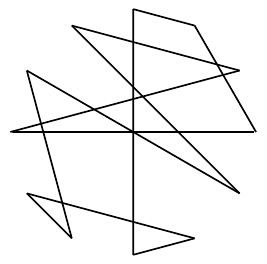
\includegraphics{Serialismo-matematicas-diagrama-3}
			\end{center}
		\end{figure}
		Ahora calcularemos los espectros formados mediante todas las transformaciones del grupo generado por $\{S,\ T,\ V,\ C\}$; es decir, por ${D}_{n}\times {D}_{n}$. Volviendo a la representaci�n mediante diagramas de reloj, el problema es equivalente a averiguar cu�ntos diagramas distintos, sin n�meros ni flechas, se pueden dibujar. La flecha indica lo transformado por $V$ y $C$, mientras que los n�meros indican lo transformado por $S$ y $T$. Un diagrama sin estos dos elementos representa entonces todo un espectro serial. ¿Cu�ntos diagramas esencialmente distintos hay? De nuevo, por el lema de Burnside:
		\[\#\mbox{Espectros}=\frac{1}{|{D}_{n}\times{D}_{n}|}\sum_{\sigma\in{S}_n}|{Stab}(\sigma)|=\frac{1}{2n\cdot2n}\sum_{\sigma\in{S}_n}|{Stab}(\sigma)|\]
		
		En vez de expresar el sumatorio como ``para cada $\sigma$, el n�mero de $\Psi$ que fijan $\sigma$'', se puede expresar como ``para cada $\Psi$, el n�mero de $\sigma$ fijados por $\Psi$''. La f�rmula queda de esta manera:
		
		\[\#\mbox{Espectros}=\frac{1}{4n^2}\sum_{\Psi\in{D}_{n}\times{D}_{n}}{Fij}(\Psi)\] 
		
		Ahora hay que averiguar para cada elemento de ${D}_{n}\times{D}_{n}$ cu�ntas series estabiliza. Por ejemplo, trivialmente no hay permutaciones estables mediante $C$ y $V$ solamente.
		
		
		\subsubsection[Elementos estables mediante $T$]{Elementos estables mediante ${T}$}
		
		Los elementos estables mediante $T^{k}$ son a los que, tras aplicar una rotaci�n de $\uptheta_{k}=\frac{2\pi k}{n}$, para $1\leq k\leq n$, quedan igual. Por tanto, los sumandos que aportan a la suma total son $\sum\limits_{k=1}^{n}{Fij}(\uptheta_{k})$.
		
		Por otro lado, si $1\leq p,q\leq n$ y $gcd(p,n)=gcd(q,n)$ entonces ${Fij}(\uptheta_p)={Fij}(\uptheta_q)$, ya que por el lema de B�zout lo que genera la rotaci�n $\uptheta_p$ es igual a lo que genera la rotaci�n $\uptheta_{{gcd}(p,n)}$. Esto permite que se puedan agrupar los sumandos con igual m�ximo com�n divisor con respecto a $n$. Es decir, $\sum\limits_{k=1}^{n}{Fij}(\uptheta_{k})=\sum\limits_{d|n}\left(\mathcal{C}\cdot{Fij}(\uptheta_d)\right)$, con $d$ divisor de $n$.
		Por ejemplo, si $n=6$:
		\begin{align*}
			&{Fij}(\uptheta_{1})+{Fij}(\uptheta_{2})+{Fij}(\uptheta_{3})+{Fij}(\uptheta_{4})+{Fij}(\uptheta_{5})+{Fij}(\uptheta_{6})=\\
			&{Fij}(\uptheta_{1})+{Fij}(\uptheta_{2})+{Fij}(\uptheta_{3})+{Fij}(\uptheta_{2})+{Fij}(\uptheta_{1})+{Fij}(\uptheta_{6})=\\
			&2\cdot{Fij}(\uptheta_{1})+2\cdot{Fij}(\uptheta_{2})+1\cdot{Fij}(\uptheta_{3})+1\cdot{Fij}(\uptheta_{6})
		\end{align*}
		
		
		Ahora queremos encontrar el coeficiente $\mathcal{C}$ de ${Fij}(\uptheta_d)$, es decir, el n�mero de $k\leq n$ con igual m�ximo com�n divisor $d$. Pero que $k\leq n$ y $gcd(k,n)=d$ es equivalente a que $ \frac{k}{d}\leq\frac{n}{d}$ y $gcd\left(\frac{k}{d},\frac{n}{d}\right)=1$. Por tanto, el n�mero de $k$ con m�ximo comun divisor $d$ es $\varphi\left(\frac{n}{d}\right)$. La funci�n $\varphi(x)$ se llama la funci�n \textit{phi} de Euler, y muestra precisamente la cantidad de n�meros menores que �l y coprimos con �l. Entonces $\sum\limits_{{k}=1}^{n}{Fij}(\uptheta_{{k}})=\sum\limits_{d|n}\left(\varphi(\frac{n}{d})\cdot{Fij}(\uptheta_d)\right)$.
		
		Para calcular ${Fij}(\uptheta_d)$ hay que analizar c�mo se construyen los diagramas invariantes respecto a una rotaci�n. Estos diagramas deben tener varios \textit{ciclos} iguales entre s� \textemdash para que queden invariantes al rotarlos\textemdash~pero cada uno desde un punto distinto: desde cada m�ltiplo de $d$. El n�mero de ciclos es, por tanto, $\frac{n}{d}$.
		
		Al construir uno de estos diagramas, se escoge la primera nota entre las $n$. Despu�s se escoge la segunda, pero no se pueden escoger los v�rtices m�ltiplos de $d$ (de los que hay $\frac{n}{d}$), ya que van a ser el comienzo de los sucesivos ciclos. Hay entonces $n-\frac{n}{d}$ posibilidades. Despu�s se escoge la tercera, pero sin escoger los m�ltiplos de $d$ ni los m�ltiplos de $d\ +$ la segunda posici�n. Hay $n - 2\cdot\frac{n}{d}$ posibilidades, y as� sucesivamente hasta terminar el primer ciclo:
		\[n\left(n-\frac{n}{d}\right)\left(n-\frac{2n}{d}\right)\cdots\left(n-\frac{(d-1)n}{d}\right)=\] 
		\[=n^d\left(1-\frac{1}{d}\right)\left(1-\frac{2}{d}\right)\cdots\left(1-\frac{d-1}{d}\right)=\]
		\[=n^d\left(\frac{d-1}{d}\right)\left(\frac{d-2}{d}\right)\cdots\left(\frac{1}{d}\right)=n^d\cdot\frac{(d-1)!}{d^{d-1}}\cdot\frac{d}{d}=\left(\frac{n}{d}\right)^d\cdot d!\]
		
		Por ejemplo, si $d=2$ y $n=8$, supongamos que escogemos el punto 0$^{(0)}$ como el primero. Despu�s, si cogi�ramos alguno de los puntos 0$^{(*)}$ luego no podr�amos tener simetr�a al rotarlo un �ngulo de $\uptheta_2$. Entonces hay que escoger alguno de los 1$^{(*)}$. Supongamos que es 1$^{(1)}$. En este ejemplo nuestro \textit{ciclo} quedar�a de la siguiente manera:
		
%		\begin{figure}[h]
			\begin{center}
%				\begin{tikzpicture}
%			\node [draw,circle,inner sep=0,minimum height=2cm] at (0,0) {};
%			\foreach\y in {0,1,2,3} {
%				\foreach\x in {0,1} {
%					\draw[thin] (90-45*\x-90*\y:0.85) -- (90-45*\x-90*\y:1.35) node[fill=white,inner sep=0pt] {\x$^{(\y)}$};
%				}
%			}
%			\draw (90:1) -- (-45:1);
%			\end{tikzpicture}
			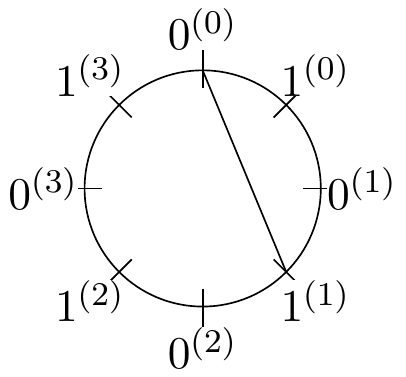
\includegraphics{Serialismo-matematicas-diagrama-4}
			\end{center}
%		\end{figure}
		
		Para escoger el segundo ciclo, su primera nota debe caer en el conjunto de v�rtices m�ltiplos de $d$ \textemdash de los que hay $\frac{n}{d}$. En el ejemplo ser�an los 0$^{(*)}$. Sin embargo, no podr�a ser cualquier m�ltiplo, ya que si se escoge uno con posici�n no coprima, el pol�gono se cerrar�a antes de tiempo sin pasar por todos los v�rtices. Entonces hay que escoger entre los v�rtices coprimos, de los que hay $\varphi\left(\frac{n}{d}\right)$. Tras esto el pol�gono est� totalmente determinado, y se puede formar de $\sum\limits_{d|n}\left(\varphi^2(\frac{n}{d})\cdot\left(\frac{n}{d}\right)^d\cdot d!\right)$ maneras.
		
		En nuestro ejemplo, si escogemos el siguiente comienzo del ciclo como el 0$^{(2)}$, como 2 no es coprimo con $\frac{n}{d}=4$, quedar�a de esta manera:
		
		\begin{center}
%			\begin{multicols}{2}
%				\begin{tikzpicture}
%				\node [draw,circle,inner sep=0,minimum height=2cm] at (0,0) {};
%				\foreach\y in {0,1,2,3} {
%					\foreach\x in {0,1} {
%						\draw[thin] (90-45*\x-90*\y:0.85) -- (90-45*\x-90*\y:1.35) node[fill=white,inner sep=0pt] {\x$^{(\y)}$};
%					}
%				}
%				\draw (90:1) -- (-45:1) -- (-90:1);
%				\end{tikzpicture}
%				
%				\begin{tikzpicture}
%				\node [draw,circle,inner sep=0,minimum height=2cm] at (0,0) {};
%				\foreach\y in {0,1,2,3} {
%					\foreach\x in {0,1} {
%						\draw[thin] (90-45*\x-90*\y:0.85) -- (90-45*\x-90*\y:1.35) node[fill=white,inner sep=0pt] {\x$^{(\y)}$};
%					}
%				}
%				\draw (90:1) -- (-45:1) -- (-90:1);
%				\draw[rotate=-180] (90:1) -- (-45:1) -- (-90:1);
%				\end{tikzpicture}
%			\end{multicols}
		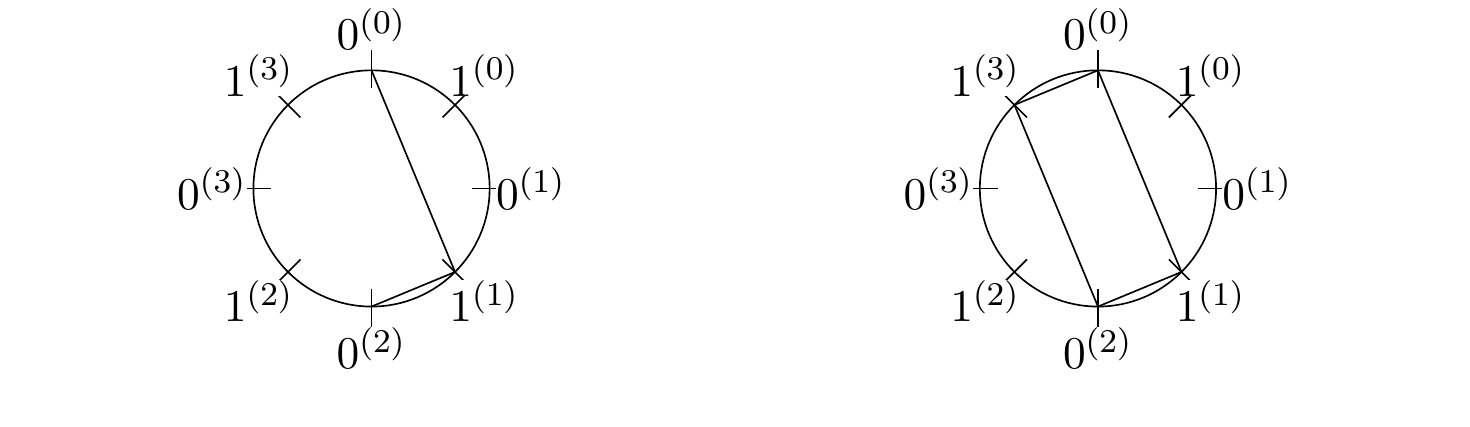
\includegraphics{Serialismo-matematicas-diagrama-5}
		\end{center}

		Efectivamente, el diagrama se cierra antes de pasar por todos los v�rtices. En cambio, si escogemos 0$^{(1)}$:
%		\begin{multicols}{4}			
%			\begin{tikzpicture}
%			\node [draw,circle,inner sep=0,minimum height=2cm] at (0,0) {};
%			\foreach\y in {0,1,2,3} {
%				\foreach\x in {0,1} {
%					\draw[thin] (90-45*\x-90*\y:0.85) -- (90-45*\x-90*\y:1.35) node[fill=white,inner sep=0pt] {\x$^{(\y)}$};
%				}
%			}
%		\draw (90:1) -- (-45:1) -- (0:1);
%%		\draw[rotate=-90] (90:1) -- (-45:1) -- (0:1);
%%		\draw[rotate=180] (90:1) -- (-45:1) -- (0:1);
%%		\draw[rotate=90] (90:1) -- (-45:1) -- (0:1);
%			\end{tikzpicture}
%			
%			\begin{tikzpicture}
%			\node [draw,circle,inner sep=0,minimum height=2cm] at (0,0) {};
%			\foreach\y in {0,1,2,3} {
%				\foreach\x in {0,1} {
%					\draw[thin] (90-45*\x-90*\y:0.85) -- (90-45*\x-90*\y:1.35) node[fill=white,inner sep=0pt] {\x$^{(\y)}$};
%				}
%			}
%			\draw (90:1) -- (-45:1) -- (0:1);
%			\draw[rotate=-90] (90:1) -- (-45:1) -- (0:1);
%%			\draw[rotate=180] (90:1) -- (-45:1) -- (0:1);
%%			\draw[rotate=90] (90:1) -- (-45:1) -- (0:1);
%			\end{tikzpicture}
%			
%			\begin{tikzpicture}
%			\node [draw,circle,inner sep=0,minimum height=2cm] at (0,0) {};
%			\foreach\y in {0,1,2,3} {
%				\foreach\x in {0,1} {
%					\draw[thin] (90-45*\x-90*\y:0.85) -- (90-45*\x-90*\y:1.35) node[fill=white,inner sep=0pt] {\x$^{(\y)}$};
%				}
%			}
%			\draw (90:1) -- (-45:1) -- (0:1);
%			\draw[rotate=-90] (90:1) -- (-45:1) -- (0:1);
%			\draw[rotate=180] (90:1) -- (-45:1) -- (0:1);
%%			\draw[rotate=90] (90:1) -- (-45:1) -- (0:1);
%			\end{tikzpicture}
%			
%			\begin{tikzpicture}
%			\node [draw,circle,inner sep=0,minimum height=2cm] at (0,0) {};
%			\foreach\y in {0,1,2,3} {
%				\foreach\x in {0,1} {
%					\draw[thin] (90-45*\x-90*\y:0.85) -- (90-45*\x-90*\y:1.35) node[fill=white,inner sep=0pt] {\x$^{(\y)}$};
%				}
%			}
%			\draw (90:1) -- (-45:1) -- (0:1);
%			\draw[rotate=-90] (90:1) -- (-45:1) -- (0:1);
%			\draw[rotate=180] (90:1) -- (-45:1) -- (0:1);
%			\draw[rotate=90] (90:1) -- (-45:1) -- (0:1);
%			\end{tikzpicture}
%		\end{multicols}
\begin{center}
	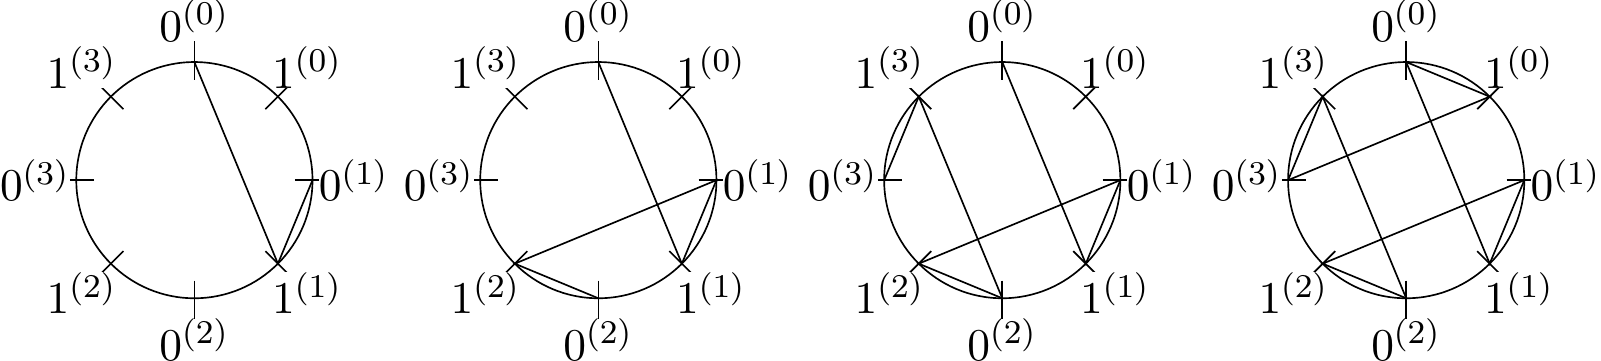
\includegraphics{Serialismo-matematicas-diagrama-6}
\end{center}
	
		Y con 0$^{(3)}$:
%		\begin{multicols}{4}			
%			\begin{tikzpicture}
%			\node [draw,circle,inner sep=0,minimum height=2cm] at (0,0) {};
%			\foreach\y in {0,1,2,3} {
%				\foreach\x in {0,1} {
%					\draw[thin] (90-45*\x-90*\y:0.85) -- (90-45*\x-90*\y:1.35) node[fill=white,inner sep=0pt] {\x$^{(\y)}$};
%				}
%			}
%			\draw (90:1) -- (-45:1) -- (180:1);
%	%		\draw[rotate=-90] (90:1) -- (-45:1) -- (180:1);
%	%		\draw[rotate=180] (90:1) -- (-45:1) -- (180:1);
%	%		\draw[rotate=90] (90:1) -- (-45:1) -- (180:1);
%			\end{tikzpicture}
%			
%			\begin{tikzpicture}
%			\node [draw,circle,inner sep=0,minimum height=2cm] at (0,0) {};
%			\foreach\y in {0,1,2,3} {
%				\foreach\x in {0,1} {
%					\draw[thin] (90-45*\x-90*\y:0.85) -- (90-45*\x-90*\y:1.35) node[fill=white,inner sep=0pt] {\x$^{(\y)}$};
%				}
%			}
%			\draw (90:1) -- (-45:1) -- (180:1);
%			\draw[rotate=-90] (90:1) -- (-45:1) -- (180:1);
%	%		\draw[rotate=180] (90:1) -- (-45:1) -- (180:1);
%	%		\draw[rotate=90] (90:1) -- (-45:1) -- (180:1);
%			\end{tikzpicture}
%			
%			\begin{tikzpicture}
%			\node [draw,circle,inner sep=0,minimum height=2cm] at (0,0) {};
%			\foreach\y in {0,1,2,3} {
%				\foreach\x in {0,1} {
%					\draw[thin] (90-45*\x-90*\y:0.85) -- (90-45*\x-90*\y:1.35) node[fill=white,inner sep=0pt] {\x$^{(\y)}$};
%				}
%			}
%			\draw (90:1) -- (-45:1) -- (180:1);
%			\draw[rotate=-90] (90:1) -- (-45:1) -- (180:1);
%			\draw[rotate=180] (90:1) -- (-45:1) -- (180:1);
%	%		\draw[rotate=90] (90:1) -- (-45:1) -- (180:1);
%			\end{tikzpicture}
%			
%			\begin{tikzpicture}
%			\node [draw,circle,inner sep=0,minimum height=2cm] at (0,0) {};
%			\foreach\y in {0,1,2,3} {
%				\foreach\x in {0,1} {
%					\draw[thin] (90-45*\x-90*\y:0.85) -- (90-45*\x-90*\y:1.35) node[fill=white,inner sep=0pt] {\x$^{(\y)}$};
%				}
%			}
%			\draw (90:1) -- (-45:1) -- (180:1);
%			\draw[rotate=-90] (90:1) -- (-45:1) -- (180:1);
%			\draw[rotate=180] (90:1) -- (-45:1) -- (180:1);
%			\draw[rotate=90] (90:1) -- (-45:1) -- (180:1);
%			\end{tikzpicture}
%		\end{multicols}
\begin{center}
		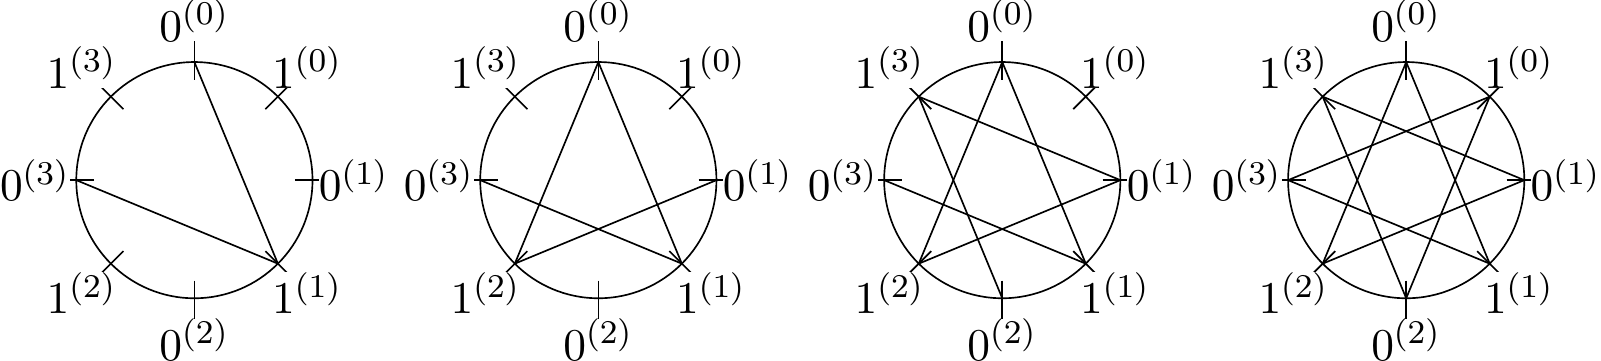
\includegraphics{Serialismo-matematicas-diagrama-7}
\end{center}
		
		Sea $d=3$ y $n=6$. Escogiendo el primer n�mero como 0$^{(0)}$, el segundo como 1$^{(0)}$ y el tercero como 2$^{(1)}$, no queda m�s remedio que escoger como comienzo del segundo ciclo el 0$^{(1)}$.
		
%	\begin{multicols}{3}
%		\begin{tikzpicture}
%		\node [draw,circle,inner sep=0,minimum height=2cm] at (0,0) {};
%		\foreach\y in {0,1} {
%			\foreach\x in {0,1,2} {
%				\draw[thin] (90-60*\x-180*\y:0.85) -- (90-60*\x-180*\y:1.35) node[fill=white,inner sep=0pt] {\x$^{(\y)}$};
%			}
%		}
%		\draw (90:1) -- (30:1) -- (150:1);
%		\end{tikzpicture}
%		
%		\begin{tikzpicture}
%		\node [draw,circle,inner sep=0,minimum height=2cm] at (0,0) {};
%		\foreach\y in {0,1} {
%			\foreach\x in {0,1,2} {
%				\draw[thin] (90-60*\x-180*\y:0.85) -- (90-60*\x-180*\y:1.35) node[fill=white,inner sep=0pt] {\x$^{(\y)}$};
%			}
%		}
%		\draw (90:1) -- (30:1) -- (150:1) -- (-90:1);
%		%		\draw[rotate=180] (90:1) -- (30:1) -- (150:1) -- (-90:1);
%		\end{tikzpicture}
%		
%		\begin{tikzpicture}
%		\node [draw,circle,inner sep=0,minimum height=2cm] at (0,0) {};
%		\foreach\y in {0,1} {
%			\foreach\x in {0,1,2} {
%				\draw[thin] (90-60*\x-180*\y:0.85) -- (90-60*\x-180*\y:1.35) node[fill=white,inner sep=0pt] {\x$^{(\y)}$};
%			}
%		}
%		\draw (90:1) -- (30:1) -- (150:1) -- (-90:1);
%		\draw[rotate=180] (90:1) -- (30:1) -- (150:1) -- (-90:1);
%		\end{tikzpicture}
%	\end{multicols}
\begin{center}
	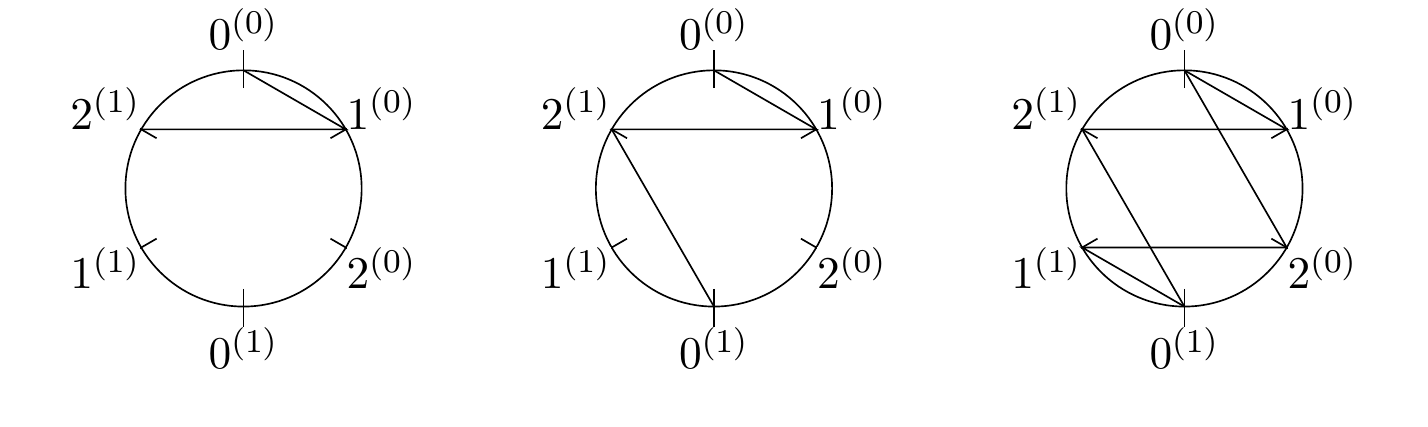
\includegraphics{Serialismo-matematicas-diagrama-8}
\end{center}

		Pero tambi�n podr�a aparecer este mismo comienzo con la parte final dada la vuelta, sim�trica, de esta manera: 0$^{(0)}$, 1$^{(0)}$, 2$^{(1)}$, 2$^{(0)}$, 1$^{(1)}$, 0$^{(1)}$. Esta construcci�n no est� incluida en lo descrito anteriormente, y sin embargo es invariante con respecto a T, V y C a la vez. 
		
%		\begin{multicols}{3}
%			\begin{tikzpicture}
%			\node [draw,circle,inner sep=0,minimum height=2cm] at (0,0) {};
%			\foreach\y in {0,1} {
%				\foreach\x in {0,1,2} {
%					\draw[thin] (90-60*\x-180*\y:0.85) -- (90-60*\x-180*\y:1.35) node[fill=white,inner sep=0pt] {\x$^{(\y)}$};
%				}
%			}
%			\draw (90:1) -- (30:1) -- (150:1);
%			\end{tikzpicture}
%			
%			\begin{tikzpicture}
%			\node [draw,circle,inner sep=0,minimum height=2cm] at (0,0) {};
%			\foreach\y in {0,1} {
%				\foreach\x in {0,1,2} {
%					\draw[thin] (90-60*\x-180*\y:0.85) -- (90-60*\x-180*\y:1.35) node[fill=white,inner sep=0pt] {\x$^{(\y)}$};
%				}
%			}
%			\draw (90:1) -- (30:1) -- (150:1);
%			\draw[rotate=180] (90:1) -- (30:1) -- (150:1);
%			\end{tikzpicture}
%			
%			\begin{tikzpicture}
%			\node [draw,circle,inner sep=0,minimum height=2cm] at (0,0) {};
%			\foreach\y in {0,1} {
%				\foreach\x in {0,1,2} {
%					\draw[thin] (90-60*\x-180*\y:0.85) -- (90-60*\x-180*\y:1.35) node[fill=white,inner sep=0pt] {\x$^{(\y)}$};
%				}
%			}
%			\draw (90:1) -- (30:1) -- (150:1);
%			\draw[rotate=180] (90:1) -- (30:1) -- (150:1);
%			\draw[] (-90:1) -- (90:1);
%			\draw[] (150:1) -- (-30:1);
%			\end{tikzpicture}
%		\end{multicols}
\begin{center}
		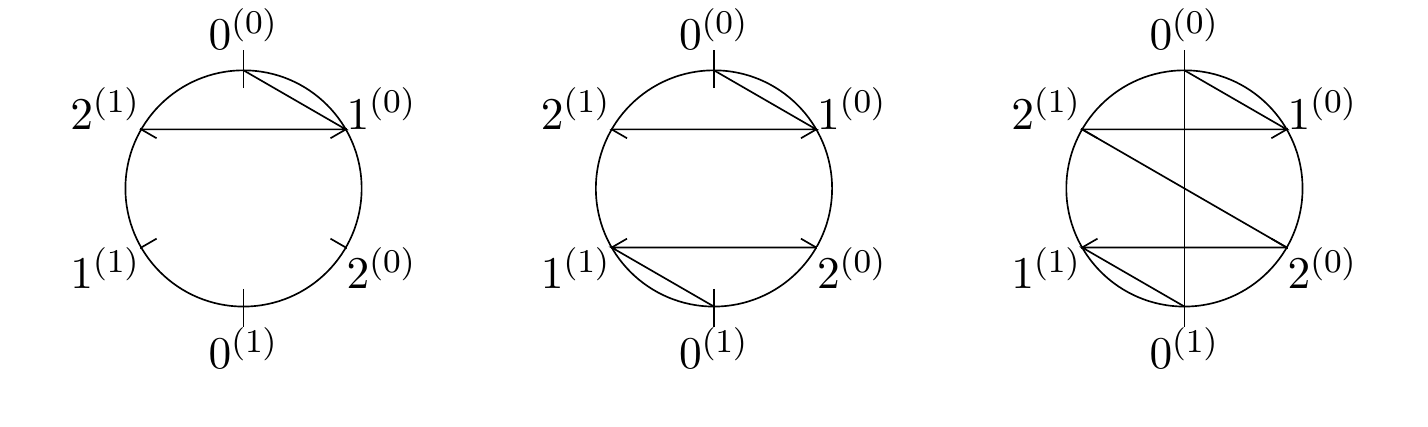
\includegraphics{Serialismo-matematicas-diagrama-9}
\end{center}
		
		Y es que con $n$ par, al rotar $\uptheta_{{n}/{2}}$ el diagrama, �ste puede llegar con la orientaci�n cambiada. Esto puede ocurrir cuando haya una diagonal; es decir, cuando entre dos notas haya un intervalo de $\frac{n}{2}$.
		
		\begin{center}
%		\begin{tikzpicture}[ddiagram]
%		\ddiagram[no tikz]{0,1,5,2,4,3}
%		
%		\draw[style=ddihedralArrow] (2.5,0) -- node[above=5pt] {T$^3$} (4,0);
%		
%		\ddiagram[no tikz, xshift=4cm]{3,4,2,5,1,0}
%		
%		\draw[style=ddihedralArrow,xshift=6cm] (2.5,0) -- node[above=5pt] {V} (4,0);
%		
%		\ddiagram[no tikz, xshift=8cm, arrow shift=1.25]{3,0,1,5,2,4}
%		
%		\draw[style=ddihedralArrow] (12.3,-2.5) -- (12.3,-3.25) -- node [fill=white] {C} (0,-3.25) -- (0,-2.5);
%		\end{tikzpicture}
		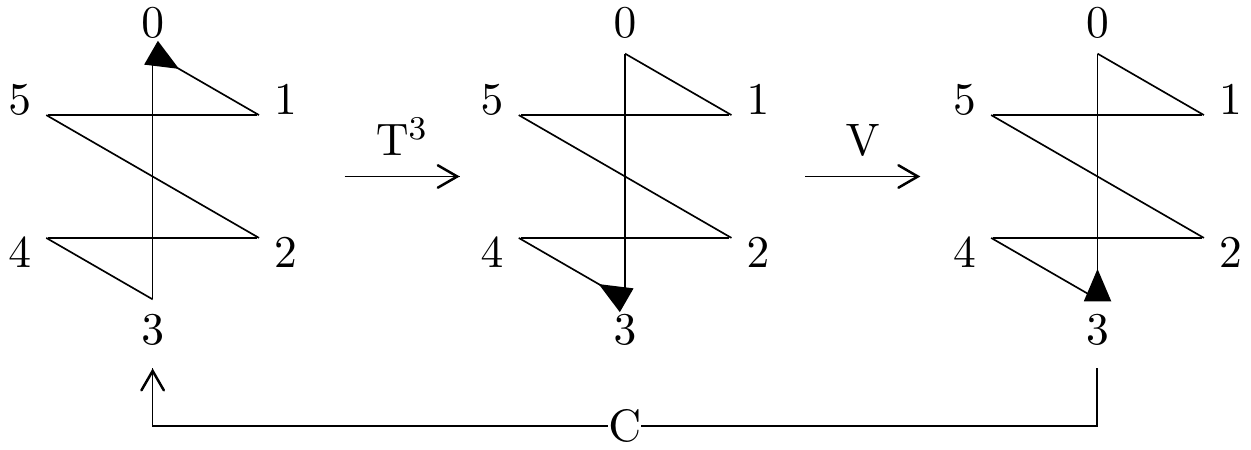
\includegraphics{Serialismo-matematicas-diagrama-10}
		\end{center}
		
		Se escoge el primer punto de entre $\frac{n}{2}$ posibilidades. No son $n$ ya que saldr�a la misma figura si se escoge el punto antipodal.
		Con una rotaci�n de $\uptheta_{{n}/{2}}$, el primer ciclo se escoge igual que antes, de $\left(\frac{n}{n/2}\right)^{\frac{n}{2}}\cdot \frac{n}{2}!=2^{\frac{n}{2}}\cdot \frac{n}{2}!$ maneras. Y con esto ya queda la figura determinada. Esto lleva a las $\frac{n}{2}\cdot2^{\frac{n}{2}}\cdot\frac{n}{2}!$ formas de dibujar un pol�gono con las caracter�sticas buscadas.
		
		\subsubsection[Elementos estables mediante $S$]{Elementos estables mediante ${S}$}
		
		Los elementos estables mediante $S$ son aquellos que quedan invariantes mediante reflexiones. En este punto se ha de separar por paridad de $n$. 
		
		Para $n$ impar, existen $n$ reflexiones para cada uno de los ejes de simetr�a que pasan por cada v�rtice. Despu�s, hay $n$ formas de escoger el primer v�rtice de la secuencia. Ahora hay $\frac{n-1}{2}$ parejas de v�rtices; se escoge los primeros miembros entre ellos de $2^{\frac{n-1}{2}}$ formas, tras lo cual �stos se ordenan de $\frac{n-1}{2}!$ formas. Esto da un resultado de  $n^2\cdot2^{\frac{n-1}{2}}\cdot\frac{n-1}{2}!$ pol�gonos invariantes.
		
		Para $n$ par se tienen dos simetr�as: con ejes que pasan por v�rtices y con ejes que pasan por lados. De manera similar a la anterior, se escoge el eje, el primer v�rtice, los primeros miembros de las parejas de v�rtices y se ordenan. Para las simetr�as con ejes que pasan por v�rtices, da un resultado de  $\frac{n^2}{2}\cdot2^{\frac{n}{2}}\cdot\left(\frac{n}{2}-1\right)!$. Para las simetr�as con ejes que pasan por lados, da un resultado de $\frac{n^2}{2}\cdot2^{\frac{n}{2}-1}\cdot\frac{n}{2}!$.
		
		\subsubsection*{Suma completa}
		
		En resumen, estos a continuaci�n son los numeradores $\sum%_{\Psi\in\mbox{D}_{n}\times\mbox{D}_{n}}
		{Fij}(\Psi)$. El resultado final del n�mero de diagramas posibles, o espectros seriales distintos, es dicho numerador entre $4n^2$, el tama�o del grupo. 	
		\def\arraystretch{1.5}
		\[\begin{array}{c||c}
		&\textbf{\textit{n} IMPAR}\\\hline\hline
		\mbox{Rotaci�n}&\sum\limits_{d|n}\left(\varphi^2(\frac{n}{d})\cdot\left(\frac{n}{d}\right)^d\cdot d!\right)\\\hline
		\mbox{Reflexi�n}&n^2\cdot2^{\frac{n-1}{2}}\cdot\frac{n-1}{2}!\\\hline
		&\sum\limits_{d|n}\left(\varphi^2(\frac{n}{d})\cdot\left(\frac{n}{d}\right)^d\cdot d!\right)+n^2\cdot2^{\frac{n-1}{2}}\cdot\frac{n-1}{2}!\\
		\end{array}\]
		
		\[\begin{array}{c||c}
		&\textbf{\textit{n} PAR}\\\hline\hline
		\mbox{Rotaci�n I}&\sum\limits_{d|n}\left(\varphi^2(\frac{n}{d})\cdot\left(\frac{n}{d}\right)^d\cdot d!\right)\\\hline
		\mbox{Rotaci�n II}&\frac{n}{2}\cdot2^{\frac{n}{2}}\cdot\frac{n}{2}!\\\hline
		\mbox{Reflexi�n v�rtices}&\frac{n^2}{2}\cdot2^{\frac{n}{2}}\cdot\left(\frac{n}{2}-1\right)!\\\hline
		\mbox{Reflexi�n lados}&\frac{n^2}{2}\cdot2^{\frac{n}{2}-1}\cdot\frac{n}{2}!\\\hline
		&\sum\limits_{d|n}\left(\varphi^2(\frac{n}{d})\cdot\left(\frac{n}{d}\right)^d\cdot d!\right)+\frac{n(n+6)}{4}\cdot2^{\frac{n}{2}}\cdot\frac{n}{2}!\\
		\end{array}\]
		\def\arraystretch{1}
		
	\subsection{Medefonismo, monofonismo y difonismo}
	\label{s:trivcase}
		Con $n=0$ se da el caso de medefonismo. El grupo sim�trico de orden 0 tiene $0!=1$ elemento. Por tanto, hay una sola posible serie, $\sigma$, que es la que no tiene ninguna nota. El medefonismo es com�nmente llamado silencio.
		
%		\[\sigma=\drow{}
%		\qquad\qquad\qquad
%		\begin{array}{l||r}
%		&\\
%		\hline
%		\hline
%		&\\
%		\hline
%		&
%		\end{array}\]
\begin{center}
			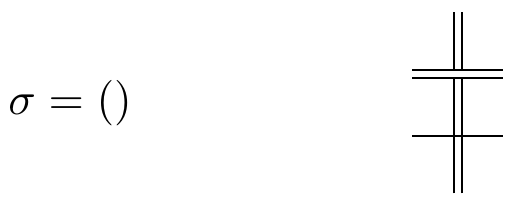
\includegraphics{Serialismo-matematicas-diagrama-11}
\end{center}
	
		Con $n=1$ se da el caso de monofonismo. Con solamente una posible nota, el grupo sim�trico de orden 1 tiene $1!=1$ elemento. Por tanto, hay una sola posible serie, $\sigma_0$, que es igual a su inversa, a su retrogradaci�n y a su retrogradaci�n inversa:
		
%		\[\sigma_0=\drow{0}
%		\qquad\qquad\qquad
%		\begin{array}{l|c|r}
%			&{I}_{0}&\\
%			\hline
%			{T}_{0}&0&{R}_{0}\\
%			\hline
%			&{IR}_{0}&\\
%			\hline
%			&{RI}_{0}&
%		\end{array}\]
\begin{center}
					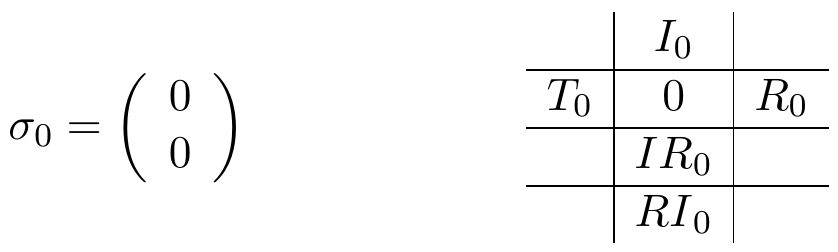
\includegraphics{Serialismo-matematicas-diagrama-12}
\end{center}
	
		Con $n=2$ se da el caso de difonismo. Tiene dos posibles notas, as� que su grupo sim�trico, el de orden 2, tiene $2!=2$ elementos. Por tanto, hay dos series distintas, $\sigma_0$ y $\sigma_1$. Se puede observar que ambas pertenecen al mismo espectro serial, dado que $\sigma_1={T}^1(\sigma_0)$. Adem�s, al igual que en el monofonismo, ambas coinciden con sus inversas, incumpliendo la regla general para $n>2$ probada en el apartado \ref{s:itr}.
		
%		\[\sigma_0=\drow{0,1}
%		\qquad\qquad
%		\begin{array}{l|cc|r}
%			&{I}_{0}&{I}_{1}&\\
%			\hline
%			{T}_{0}&0&1&{R}_{0}\\
%			{T}_{1}&1&0&{R}_{1}\\
%			\hline
%			&{IR}_{0}&{IR}_{1}&\\
%			\hline
%			&{RI}_{0}&{RI}_{1}&
%		\end{array}
%		\qquad\qquad
%		\sigma_1=\drow{1,0}\]
\begin{center}
					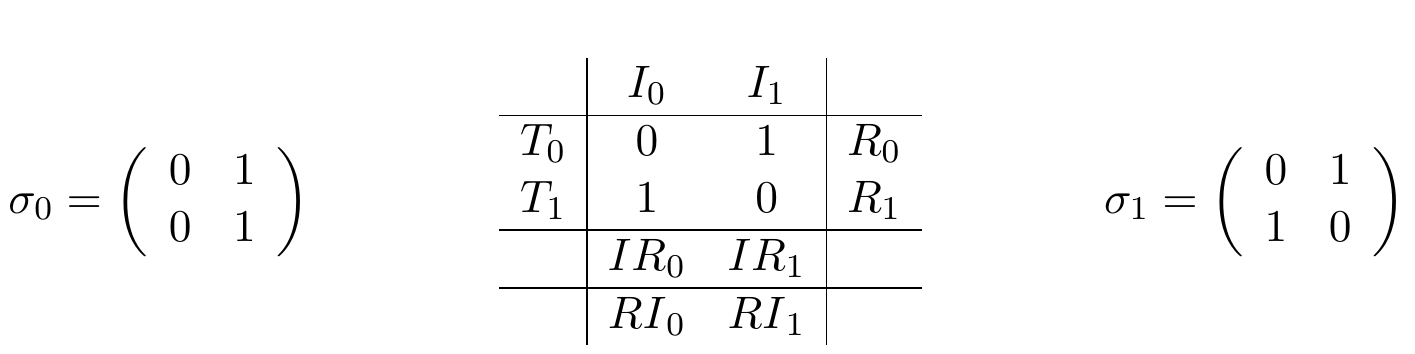
\includegraphics{Serialismo-matematicas-diagrama-13}
\end{center}

    
    \part{MODIFICACIONES}
	\chapter{EL SERIALISMO EN LA FILOSOFÍA DEL ARTE}\label{ch:filosofia}
	 % TODO
        % 08.Recorrido filosófico histórico, filosofía del arte (quotes), motivos míos (filosofía actual)
    \section{Recorrido filosófico del serialismo}
    Schoenberg thought 'classical' tonality (aka. common-practise) was a social construct, every law was arbitrary, and that people enjoyed that kind of music because the system had internal consistency. Therefore, he created a new system (12-tone) that in his opinion had the same logic. He believed that in 100 years lay people would be singing his tunes!!
    
    Some aspects of traditional tonality *are* arbitrary, e.g. Why are maj./min. chords consonant but 7ths and 9ths not? We could move the line and say that 7ths are consonant too but 9ths still not, etc. Also, we could use scales from 'foreign' musical traditions, like the acoustic scale, and so on.
    
    Studies show that some concepts are universal. E.g. unrelated cultures like Scotland and China have pentatonic melodies (c-d-e-g-a). That's not a coincidence, most scales around the world share certain properties. In no culture is the octave split in equal intervals (e.g.12), and are all the notes treated equally.
    
    Debussy, Ravel, and Stravinsky used uncommon scales, harmonies (no tonic/dominant chords...), and rhythms; but they're still popular because they followed some of the musical universals. Also, Indian Ragas, Arabic Maqam, and Blues melodies don't follow traditional tonality, but they can be easily grasped.
    
    Scriabin too used dissonance and ambiguity, but he isn't atonal in Schoenberg's sense. He mostly used the octatonic scale (used in Jazz, a 'popular' genre), and the acoustic scale (like the Simpsons theme!!). He uses 7 and 8-note scales, not all 12 tones. Also, his harmonies respect the harmonic series and follow a vague form of tonality, e.g. Vers la Flamme begins and ends with a chord built on E, and he 'modulates' by 3rds and tritones.
    
    Schoenberg and his acolytes were obsessed in making history by writing something radically new. However, I still like some of their stuff, but Berg's concerto isn't beautiful because it's serial, it's rather because he was so cunning that he could 'circumvent' the rules and write something meaningful. Nobody 'hears' a tone row. In some way, when someone says "Boulez's 2nd sonata is random notes", he's actually right, because we can't *hear* the patterns. They can only be *read* in the score. They're the emperor's clothes.
    
    
    Pensive, those are some great points. The systems of tonality vary around the world. However I disagree with you on Schoenberg's reason for developing the twelve tone system. I believe Schoenberg thought the twelve tone system was a natural developm
    
        
    Oh yeah, I was simplyfying a lot about Schoenberg. To be more exact, he (and Webern, Berg...) were first obsessed with the motif (ie. tiny melodic bit). Check out Berg's Piano Sonata: everything's based on the motifs of the very first bars. He thought that if the motif became the strutural 'glue' of a piece, then tonality was not necessary as a 'unifying' force. But that overthrow is controversial, and implies many personal circumstances... Later, he substituted the motif for the tone row as the main principle.
    
    In any case, Schoenberg's 12-tone technique was not the "natural" continuation of tonality, it was just one alternative. What makes Scriabin's or Stravinski's methods less valid? However, Schoenberg, unlike the others, wrote many many books ('selling' his ideas) that became the official textbooks of many American universities (see http://www.nytimes.com/2000/07/23/arts/l-serialist-history-textbook-dogma-297585.html)... And for a time, contradicting him became a sin (e.g. %http://www.nytimes.com/2000/07/09/arts/music-midcentury-serialists-the-bullies-or-the-besieged.html?pagewanted=all&src=pm).
    
    \section{La visión artística de Schoenberg}
    En julio de 1921, tras haber ideado los fundamentos del dodecafonismo, Schoenberg anunció a su discípulo Josef Rufer: \begin{quote}\emph{He realizado un descubrimiento que asegurará la supremacía de la música alemana durante los próximos cien años.}\end{quote}Durante la mayor parte de su vida, Schoenberg creyó que el público general acabaría aceptando la música dodecafónica del mismo modo que se habían aceptado los sistemas tonales durante siglos. No solo eso, sino que pensaba que trascurridos esos cien años los niños cantarían canciones infantiles dodecafónicas por el mundo. El dodecafonismo sería la música del mañana.
    
    Para él, la naturalidad del sistema dodecafónico residía en que era el resultado final de un proceso histórico: desde el contrapunto y el desarrollo motívico, practicado por los grandes maestros de la tradición alemana, hasta la disolución de la tonalidad, anticipada por la música postwagneriana e impresionista. Era parte de un continuo, del desarrollo de la historia de la música.
    
    \begin{quote}
    	Yo creo que la composición con doce sonidos y la que muchos llaman erróneamente «música atonal», no es el final de un viejo período, sino el comienzo de otro nuevo. Una vez más, como hace dos siglos, hay algo a lo que se llama anticuado; y una vez más, se trata de ninguna obra en particular, en , de varias obras de determinado compositor; de nuevo, no es la mayor o menor maestría de tal compositor, sino que otra vez sucede que es un estilo el condenado al ostracismo. Vuelve ve a darse a sí misma la denominación de Música Nueva e vea impulsado a evocar.
    \end{quote}

	\begin{quote}
		La composición con doce sonidos no tiene otra finalidad que la comprensión. A la vista de ciertos acontecimientos en la historia musical reciente, ésto puede causar asombro, ya que las obras escritas en este estilo no han sido entendidas a pesar del nuevo medio de organización. Por lo que, si nos olvidáramos de que nuestros contemporáneos no son los últimos jueces, sino que la historia es generalmente la que predomina, habríamos de considerar condenado este método. Pero, si bien parece aumentar las dificultades para el oyente, ésto se compensa con las penalidades del compositor. Porque no resulta fácil el componer de esta forma, sino diez veces más difícil; solo el compositor perfectamente preparado será quien componga para el oyente musical igualmente bien dispuesto.
	\end{quote}
    
    \begin{quote}
    	El método de composición con doce sonidos surgió de una necesidad.
    	
    	En los últimos cien años, el concepto de la armonía cambió enormemente mediante el desarrollo del cromatismo. La idea de que la tonalidad fundamental -o radical- predominara en la constitución de los acordes y regulara su sucesión -concepto de tonalidad- hubo de determinar primeramente el concepto de tonalidad extendida. Muy pronto resultó dudoso el que la tónica constituyese el centro permanente al que habría de corresponder toda armonía o sucesión armónica. Asimismo, resultó dudoso si la tónica que apareciese al principio, al final, o en cualquier otro lugar, tendría realmente un sentido constructivo. La armonía de Richard Wagner hubo de promover el cambio en la lógica y en la facultad constructiva de la armonía . Una de sus consecuencias fue el llamado empleo impresionista de armonías, practicado especialmente por Debussy. Sus armonías, sin ninguna significación constructiva, eran utilizadas frecuentemente con fines coloristas para expresar estados o paisajes. Paisajes y estados que, aun siendo extra-musicales, se convertirían en elementos constructivos al incorporarlos a la función emocional. De esta manera, si no en la teoría, la tonalidad fue ya destronada en la práctica. Esto solo quizá no hubiese causado un cambio radical en la técnica de la composición. Sin embargo, fue preciso tal cambio al sumársele el desarrollo que terminó con lo que yo llamo la emancipación de la disonancia.
    \end{quote}
    
    \begin{quote}
    	El oído se fue familiarizando gradualmente con gran número de disonancias, hasta que llegó a perder el miedo a su efecto «perturbador». Ya no se esperaba ninguna preparación para las disonancias de Wagner, ni resolución para las discordancias de Strauss; no nos molestaban las armonías irregulares de Debussy, ni las asperezas contrapuntísticas de los últimos compositores. Este estado de cosas condujo a un empleo más libre de las disonancias, comparable a la utilización entre los compositores clásicos de los acordes de séptima disminuida, que podían preceder o suceder a cualquier otra armonía, consonante o disonante, como si no existiese ninguna clase de disonancia. Lo que distingue las disonancias de las consonancias no es el mayor o menor grado de belleza, sino el mayor o menor grado de comprensión.
    \end{quote}
        
     
	\section{El valor intrínseco del dodecafonismo}
	Tras la muerte de Schoenberg en 1951 y durante dos décadas más, su sistema compositivo fue venerado por los compositores jóvenes más brillantes, pero después se desvaneció de las salas de conciertos y de la memoria musical colectiva. Hoy en día la música dodecafónica está muerta. Ya solo vive académicamente: como un ejemplo que estudiar del éxito de las vanguardias elitistas del siglo XX, como una antigualla en la vitrina de un museo. Pero musicalmente ya nadie la disfruta, nadie desea escucharla ni tocarla.
	
	¿Qué valor artístico tiene un arte que ya no se practica? Aún más, ¿qué valor tiene un arte que no gusta, no sólo a las mayorías desinformadas, sino incluso a los músicos más conocedores, un arte que solo gusta al propio autor y a su grupo de discípulos? El dodecafonismo emplea los recursos matemáticos con el fin de dotar de una sintaxis a la atonalidad, pero si estos no son identificables a través de la escucha, ¿cuál es entonces su cometido? ¿En qué medida afectan las reglas dodecafónicas al discurso sonoro de una pieza? Apenas es posible distinguir auditivamente una pieza meramente atonal de una dodecafónica. \cite{basomba}
	
	Si cuando se ideó tuvo un valor intrínseco, fue por haber prescindido de algunas de las preconcepciones musicales más arraigadas, como la melodía, la consonancia o la tonalidad. Pero precisamente por eso el dodecafonismo es desagradable al oído, porque toma la disonancia y la pone al frente de toda la composición. Para Schoenberg, la aprobación del público no era el objetivo de su arte, y, de hecho, el desagrado colectivo era un signo del alto nivel artístico y espiritual al que se encontraba:
	
	\begin{quote}
		\emph{La belleza es una necesidad de los mediocres.}\footnote{A. Schoenberg, \emph{Harmonielehre}, 1922.}
	\end{quote}
	\begin{quote}
		\emph{El valor de mercado es irrelevante para el valor intrínseco. Un juicio no cualificado puede como máximo decidir el valor de mercado - un valor que puede ser inversamente proporcional al valor intrínseco.}\footnote{A. Schoenberg, \emph{An Artistic Impression} (1909) en \emph{Style and Idea}, 1985.}
	\end{quote}
	\begin{quote}
		\emph{Ningún artista, ningún poeta, ningún filósofo y ningún músico, cuyo pensamiento se desenvuelve en la más alta esfera, habrá de descender a la vulgaridad para mostrarse complacientes con un eslogan tal como <<Arte para todos>>. Porque si es arte no será para todos, y si es para todos no será arte.}\footnote{A. Schoenberg, \emph{New Music, Outmoded Music, Style and Idea}, 1946.}
	\end{quote}
	
	\section{Serialismo de escalas no cromáticas}
	Tras cien años de cambios históricos transcendentales como el desarrollo de la tecnología y la globalización, la definición de arte es muy diferente a la que Schoenberg expresaba en su tiempo. El arte está cada vez más cerca del ciudadano de a pie, y se le intenta explicar y simplificar por todos los medios el arte que no entiende.
	
	Por ello, he decidido experimentar con la idea del dodecafonismo y despojarle de lo que, en mi opinión, provoca el rechazo general: la disonancia. Ya que esta proviene del cromatismo, la idea es utilizar escalas que no tengan intervalos de semitono, y con ellas crear un serialismo de menos notas. Modificaré las notas de una obra dodecafónica ya existente para que se adapte a la nueva escala utilizada, mientras que el ritmo, la duración, el timbre y las dinámicas, que siguen siendo producto del compositor original, se dejan intactas.
	
	El objetivo de este experimento es modificar algunas obras que ya están compuestas mediante el método dodecafónico, y cambiar su serialismo de doce notas por otro pseudoserialismo de menos notas. 
		\chapter{ESTUDIO DE LAS OBRAS Y ESCALAS A MODIFICAR}
    % 09.Obras y escalas a utilizar y su estudio: por qué suena mal la hexafónica.
    \section{OBRAS A MODIFICAR}
    	El objetivo de este experimento es modificar algunas obras que ya están compuestas mediante el método dodecafónico, y cambiar su serialismo de doce notas por otro pseudoserialismo de menos notas. Para abarcar distintos estilos compositivos y hacer este estudio más riguroso, se han escogido obras de los tres principales compositores dodecafónicos: Schoenberg, Berg y Webern.
        
        Sin embargo, no se han escogido obras de compositores posteriores ni serialistas integrales. Uno de los motivos es porque interesa en este estudio la relación entre los sonidos: no se modifican más que las alturas de las notas, y por tanto no importa el resto de elementos musicales. Que estén compuestos serialmente no afecta a las conclusiones de este estudio.
        
        Por otro lado, los compositores posteriores a Schoenberg todavía no han pasado al dominio público. Eso impide, por desgracia, que se pueda trabajar libremente con su música.
        
        Por último, el hecho de que cada nota tenga su propia dinámica, su propia articulación o su propio timbre hace de las obras serialistas integrales que sean difíciles de manipular. Además, como los audios están hechos mediante ordenador y no con intérpretes reales, la calidad y la intención musical de estas partituras tan complicadas nunca pueden plasmarse a la perfección.
        
    	\subsection{SCHOENBERG: \textit{Suite para piano}, OP. 25}
        	La primera obra que pasará por el algoritmo de modificación serial es la Suite para piano de Schoenberg, ya comentada en el capítulo \ref{suitechapter}. En dicha sección se estudió su serie principal, la estructura general de la obra y su razón de ser, así como su tercer movimiento en profundidad.
            
            http://www.ccarh.org/publications/data/humdrum/tonerow/files/schoenberg/schoenberg04.pc.krn
            
    	\subsection{BERG: \textit{Lied der Lulu}}
        	La gran calidad emocional de la música de Alban Berg se refleja en esta segunda obra: es una de las arias más destacadas de su segunda ópera, \textit{Lulu}. El arreglo a voz y piano fue realizado por Erwin Stein, un músico austriaco amigo y discípulo de Schoenberg.
        	
        	%argumento de la ópera
        	
        	%series utilizadas (por personaje)

BERG: LULU: PRIMARY ROW

{0,4,5,2,7,9,6,8,B,A,3,1} (Jarman)

http://www.ccarh.org/publications/data/humdrum/tonerow/files/berg/berg10.pc.krn


BERG: LULU, ACT I , SCENE XX -- PERM. (EVERY 7TH NOTE OF PRIMARY ROW)

{10,6,3,8,5,11,4,2,9,0,1,7}


BERG: LULU, ACT II, SCENE 1 -- PERM. (EVERY 5th NOTE OF PRIMARY ROW)

{10,7,1,0,9,2,4,11,5,8,3,6}
            
        % argumento de esta aria
        
        \subsection{BERG: \textit{Der Wein}}
        
        BERG: DER WEIN
        
        {2,4,5,7,9,A,1,6,8,0,B,3}
        
        http://www.ccarh.org/publications/data/humdrum/tonerow/files/berg/berg09.pc.krn
        
        Der Wein (The Wine) (1929), Concert Aria for Soprano and Orchestra
        
        Alban Berg's concert aria Der Wein (1929) is a setting of three poems from Charles Baudelaire's "Le Vin" as translated into German by Stephan George: "Die Seele des Weines" (The Wine's Soul), "Der Wein der Liebenden" (The Wine of Lovers), "Der Wein des Einsamen" (The Wine of the Lonely One). The poems express not only the happiness and confidence (real or imagined) of those who enjoy wine's restorative powers, but also wine's celebration of itself as a giver of strength to the weak, pride to the poor, and inspiration to poets.

		Appropriately, Berg's setting is lush, evoking earthly sensations through the use of jazz elements and tango rhythms in the manner so popular in Europe in the 1920s. (Compare, for example, the contemporaneous music of Kurt Weill and Paul Hindemith.) The principal twelve-tone row Berg fashioned for Der Wein lends itself to the construction of diatonic sonorities: the first six pitches comprise most of a D minor scale, while of the row's remaining six, five are part of a G flat major scale. Few of Berg's works place as apparent an emphasis on symmetry as does Der Wein. There are no breaks between the poems, and the two outer songs provide the exposition and recapitulation of a sonata-form movement. "Die Seele des Weines" consists of an orchestral introduction, first and second theme groups with a transition, and closing material. All of this music, albeit abbreviated, returns in "Der Wien des Einsamen" in the same order and is followed by a coda. Where a traditional development section might be expected, Berg instead interpolates the scherzo-like "Der Wein der Liebenden." This middle song itself falls into three sections, the third of which is a retrograde of the second. Extended palindromes of this sort reappear in Berg's opera Lulu (1935), notably in the film music of Act II.

		Der Wein was commissioned by Ruzena Herlinger, who gave the first performance of the work in Frankfurt on June 4, 1930.
		
		\subsection{WBWERN: \textit{Variations}, OP. 27}     
		
		WEBERN: OP. 27--VARIATIONS FOR PIANO
		
		{3,B,A,2,1,0,6,4,7,5,9,8}
		
		\subsection{WEBERN: \textit{3 Lieder}, OP. 18}
		
		WEBERN: OP. 18, NO. 1, "SCHATZERL KLEIN"
		
		{0,B,5,8,A,9,3,4,1,7,2,6}
		
		WEBERN: OP. 18, NO. 2, "ERLOSUNG"
		
		{6,9,5,8,4,7,3,B,2,A,1,0}
				
		WEBERN: OP. 18, NO. 3, "AVE, REGINA COELORUM"
		
		{4,3,7,6,5,B,A,2,1,0,9,8}	
		
	\section{ESCALAS Y FUNCIONES A UTILIZAR}

        Randomly generated function
        \begin{lstlisting}
        #include <iostream>
        #include <cstdlib>
        #include <algorithm>
        
        using namespace std;
        using VI = int[12];
        
        int main() {
        	srand (time(NULL));
        	VI v;
        	for (size_t i = 0; i < 12; i++)
        		v[i] = rand()%12;
        	sort(v, v+12);
        	for (size_t i = 0; i < 12; i++)
        		cout << v[i] << " ";
        	cout << "\n";
        	return 0;
        }        
        \end{lstlisting}

        Chromatic dodecaphonic scales
        \begin{lstlisting}
        #include <iostream>
        #include <cstdlib>
        
        using namespace std;
        using VI = int[12];
        
        int main() {
        	srand (time(NULL));
        	VI v = {0,1,2,3,4,5,6,7,8,9,10,11};
        	int a,b;
        	for (size_t i = 0; i < 24; i++) {
        		a = rand() % 12;
        		b = v[i%12];
        		v[i%12] = v[a];
        		v[a] = b;
        	}
        	for (size_t i = 0; i < 12; i++)
        		cout << v[i] << " ";
        	cout << "\n";
        	return 0;
        }        
        \end{lstlisting}

        Diatonic heptaphonic scales
        2212221

        Whole tone scale
        222222

        Pentatonic scales
        22323

        Octotonic scales
        21212121

        Repetición de notas en las funciones
                $$
    \begin{array}{l|rrrrrrrrrrrr}&1&2&3&4&5&6&7&8&9&10&11&12\\\hline1&&&&&&&&&&&&1\\\hline2&&&&&&2\\\hline3&&&&3\\\hline4&&&4\\\hline5&&3&2\\\hline6&&6\\\hline7&2&5\\\hline8&4&4\\\hline9&6&3\\\hline10&8&2\\\hline11&10&1\\\hline12&12&\\\end{array}
                $$

		\chapter{RESULTADOS DE LAS MODIFICACIONES}
    
    % 10.plugin de musescore, conclusiones
    \section{Página de modificaciones y plugin}
   
    He creado una página interactiva que transforma cada nota de una partitura a la nota requerida. Está escrita en Elm y el código puede encontrarse en \textit{https://gitlab.com/dodecafonismo/modificaciones}.
   
    \begin{wrapfigure}{l}{0.2\textwidth}
    	\vspace{-0.5cm}
    	\qrcode{https://modificaciones.netlify.com/}
    	\vspace{-1.5cm}
    \end{wrapfigure} Este es el enlace de la aplicación web. Sus instrucciones de uso se encuentran al final de la página. El enlace es \textit{https://modificaciones.netlify.com/}.
    
    \section{Obra de Schoenberg}
   
   	Tomando la música debussiana y las músicas orientales como referencia, he escogido la escala pentatónica para aplicarla a la Musette de la Suite para piano Op. 25 de Schoenberg. Para relacionar la escala dodecafónica con la nueva escala, se debe crear una función que relacione las notas de ambos conjuntos. Yo he tomado esta función:
   	\[\left.\begin{matrix}\text{Escala dodecafónica:}&0&1&2&3&4&5&6&7&8&9&10&11\\\text{Escala pentatónica:}&0&0&2&2&4&4&7&7&7&9&9&0\\\end{matrix}\right.\]
   	\[\left.\begin{matrix}\text{Do}&\text{Do\#}&\text{Re}&\text{Re\#}&\text{Mi}&\text{Fa}&\text{Fa\#}&\text{Sol}&\text{Sol\#}&\text{La}&\text{La\#}&\text{Si}\\\text{Do}&\text{Do}&\text{Re}&\text{Re}&\text{Mi}&\text{Mi}&\text{Sol}&\text{Sol}&\text{Sol}&\text{La}&\text{La}&\text{Do}\\\end{matrix}\right.\]
   	
   	Se puede observar que, ya que 5 no es divisor de 12, no hay una repartición equitativa, por lo que en cada serie habrá notas que aparezcan más que otras. En mi función, las notas repetidas son el Do (nota 0) y el Sol (nota 7). Además, estas notas forman el bordón de la Musette, por lo que tendrá aspecto sonoro de Do Mayor. En el Anexo , página  se encuentra la partitura de la modificación pentatónica, sin incluir las dinámicas por cuestión de simplificación, y en la pista 2 se encuentra la grabación de la misma, creada con el programa Musescore.
   	
   	Un estudio ulterior muy interesante consistiría en probar con otras funciones que repitieran notas diferentes, o probar con otras escalas como la hexafónica (de tonos enteros) o la heptafónica (las escalas tonales), y sus respectivas funciones posibles, o incluso aplicarlo a diversas obras. La extensión de mi investigación no puede abarcar ese trabajo, además de que se necesitaría un programa que aplicara automáticamente las funciones a la partitura en vez de tener que cambiar cada nota manualmente.
   	
   	Sin embargo, he hecho una prueba sobre la primera sección de la Musette con una única función de la escala hexafónica y otra de la heptafónica, para así justificar mi elección de la escala pentatónica como la mejor entre las tres.
   	
   	Con la escala hexafónica habría una repartición equitativa en la función, por lo que la obra seguiría siendo estrictamente serialista y ninguna nota sobresaldría. El problema de esta escala es que tampoco suena natural al oído, como se puede comprobar en la pista 3 (partitura en el Anexo , página ), que es la modificación hexafónica de la primera sección de la Musette con la siguiente función:
   	\[\left.\begin{matrix}\text{Escala dodecafónica:}&0&1&2&3&4&5&6&7&8&9&10&11\\\text{Escala hexafónica:}&0&0&2&2&4&4&6&6&8&8&10&10\\\end{matrix}\right.\]
   	\[\left.\begin{matrix}\text{Do}&\text{Do\#}&\text{Re}&\text{Re\#}&\text{Mi}&\text{Fa}&\text{Fa\#}&\text{Sol}&\text{Sol\#}&\text{La}&\text{La\#}&\text{Si}\\\text{Do}&\text{Do}&\text{Re}&\text{Re}&\text{Mi}&\text{Mi}&\text{Fa\#}&\text{Fa\#}&\text{Sol\#}&\text{Sol\#}&\text{La\#}&\text{La\#}\\\end{matrix}\right.\]
   	
   	Por último, la escala heptafónica tiene el problema de contener dos intervalos de semitono, por lo que la obra modificada suena también disonante. Esto se muestra en la pista 4 (partitura en el Anexo , página ), que es la modificación heptafónica de la primera sección de la Musette con la siguiente función:
   	\[\left.\begin{matrix}\text{Escala dodecafónica:}&0&1&2&3&4&5&6&7&8&9&10&11\\\text{Escala heptafónica:}&0&0&2&2&4&5&5&7&7&9&9&11\\\end{matrix}\right.\]
   	\[\left.\begin{matrix}\text{Do}&\text{Do\#}&\text{Re}&\text{Re\#}&\text{Mi}&\text{Fa}&\text{Fa\#}&\text{Sol}&\text{Sol\#}&\text{La}&\text{La\#}&\text{Si}\\\text{Do}&\text{Do}&\text{Re}&\text{Re}&\text{Mi}&\text{Fa}&\text{Fa}&\text{Sol}&\text{Sol}&\text{La}&\text{La}&\text{Si}\\\end{matrix}\right.\]	
   
    \section{Obras de Berg}
    \section{Obras de Webern}
    \section{Conclusiones}
    
       \cleardoublepage
	\appendix
	\addappheadtotoc
	\appendixpage
	\fancyhead{}
	\pagestyle{plain}
    
\begin{appendices}
		\chapter{Código para el cálculo de matrices dodecafónicas.}
	\label{app:codigo}
		
	\lstset{
		tabsize=3,
		language=C++,
		frame=lines,
		numbers=left,
		identifierstyle=\color{magenta},
%			
%		numberstyle=\tiny,
		numberstyle=\ttfamily\tiny\color[gray]{0.3},		
%		basicstyle=\footnotesize,
		basicstyle=\small\sffamily,
%		keywordstyle=\color[rgb]{0,0,1},
		keywordstyle=\bfseries\rmfamily,
%		commentstyle=\color[rgb]{0.09, 0.45, 0.27},
		commentstyle=\it,
%		stringstyle=\color{red}
		stringstyle=\mdseries\rmfamily,
%		
		xleftmargin=2pt,
		stepnumber=1,
		numbersep=5pt,
		belowcaptionskip=\bigskipamount,
		captionpos=b,
		escapeinside={*'}{'*},
		emphstyle={\bf},
		showspaces=false,
		columns=flexible,
		showstringspaces=false,
	}
		
		\newpage
		\begin{lstlisting}
	#include <iostream>
	using namespace std;
	
	const int N = 12;
	
	int main() {
	
		int s[N + 3][N + 2];
	
		for (int i = 1; i < N + 1; ++i) {
			cin >> s[1][i];
			s[i][0] = (N - s[1][i] + s[1][1]) % N;
			s[i][N + 1] = s[i][0];
			s[0][i] = (N - s[i][0]) % N;
			s[N + 1][i] = s[0][i];
			s[N + 2][i] = (N + s[0][i] + 2 * (s[1][N] - s[1][1])) % N;
		}
	
		for (int i = 2; i < N + 1; ++i) {
			for (int j = 1; j < N + 1; ++j) {
				s[i][j] = (s[1][j] + s[i][0]) % N;
			}
		}
	
		cout << "\n$$\\begin{array}{l|";
		
		for (int i = 0; i < N; ++i) {
			cout << 'c';
		}
		
		cout << "|r}&";
	
		for (int i = 1; i < N + 1; ++i){
			cout << "\\text{I}_{" << s[0][i] << "}&";
		}
		
		cout << "\\\\\\hline";
	
		for (int i = 1; i < N + 1; ++i) {
			cout << "\\text{T}_{" << s[i][0] << "}&";
			
			for (int j = 1; j < N + 1; ++j) {
				cout << s[i][j] << "&";
			}
			
			cout << "\\text{R}_{" << s[i][N + 1] << "}\\\\";
		}
	
		cout << "\\hline&";
		
		for (int i = 1; i < N + 1; ++i) {
			cout << "\\text{IR}_{" << s[N + 1][i] << "}&";
		}
	
		cout << "\\\\\\hline&";
		
		for (int i = 1; i < N + 1; ++i) {
			cout << "\\text{RI}_{" << s[N + 2][i] << "}&";
		}
	
		cout << "\\end{array}$$\n";
	
		system("PAUSE");
	
		return 0;
	}


	\end{lstlisting}
		\newpage
	\section{Paquete de \LaTeX{}: \texttt{ddphonism}}	
	\lstset{
				language=[Latex]Tex,
		%
		basicstyle=\footnotesize\sffamily,
		keywordstyle=\footnotesize\sffamily,
		identifierstyle=\footnotesize\sffamily,
		commentstyle=\footnotesize\sffamily,
		stringstyle=\footnotesize\sffamily,
		escapechar=¬,
	}
	\label{app:latex}
	
	\verb|\lstinputlisting{ddphonism.sty}|
%	\chapter{Series de la Suite Op. 25}
	\label{app:series}
	
	\newpage
	$$\text{T}^0=\left(\begin{matrix}0&1&2&3&4&5&6&7&8&9&10&11\\4&5&7&1&6&3&8&2&11&0&9&10\\\end{matrix}\right)$$
	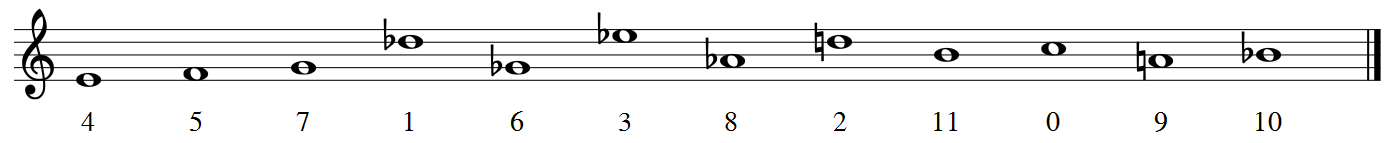
\includegraphics[width=\textwidth]{1.png}
	\bigskip\bigskip
	$$\text{T}^6=\left(\begin{matrix}0&1&2&3&4&5&6&7&8&9&10&11\\10&11&1&7&0&9&2&8&5&6&3&4\\\end{matrix}\right)$$
	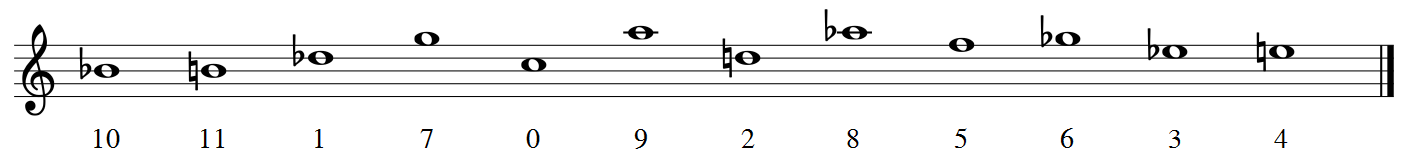
\includegraphics[width=\textwidth]{2.png}
	\bigskip\bigskip
	$$\text{IT}^0=\left(\begin{matrix}0&1&2&3&4&5&6&7&8&9&10&11\\4&3&1&7&2&5&0&6&9&8&11&10\\\end{matrix}\right)$$
	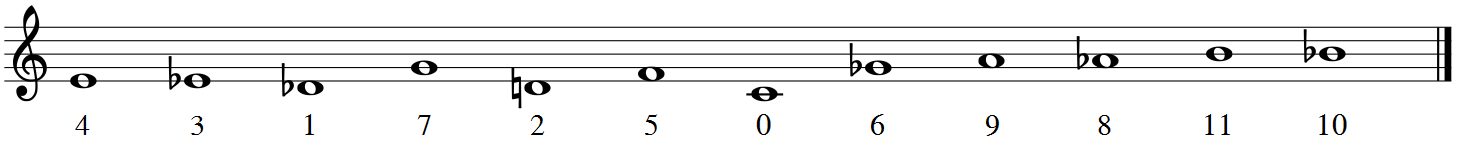
\includegraphics[width=\textwidth]{4.png}
	\bigskip\bigskip
	$$\text{IT}^6=\left(\begin{matrix}0&1&2&3&4&5&6&7&8&9&10&11\\10&9&7&1&8&11&6&0&3&2&5&4\\\end{matrix}\right)$$
	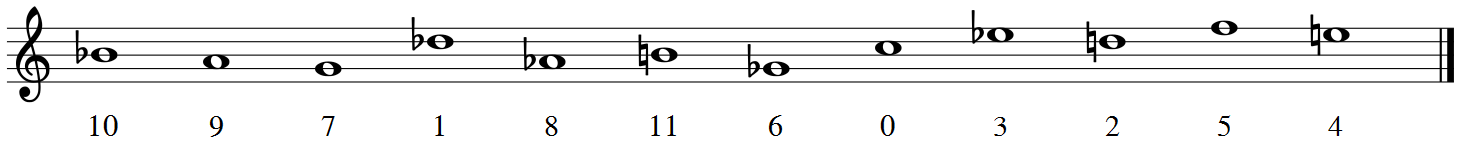
\includegraphics[width=\textwidth]{6.png}
	\newpage
	$$\text{RT}^0=\left(\begin{matrix}0&1&2&3&4&5&6&7&8&9&10&11\\10&9&0&11&2&8&3&6&1&7&5&4\\\end{matrix}\right)$$
	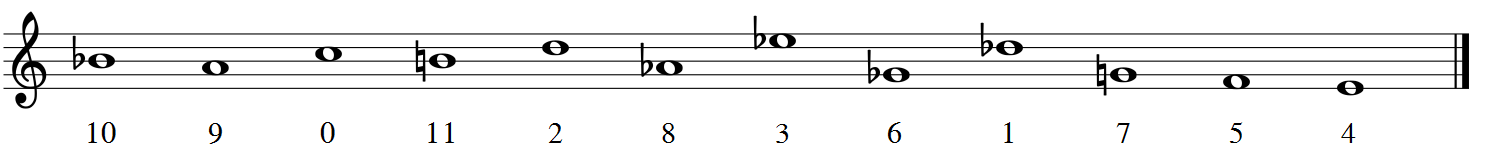
\includegraphics[width=\textwidth]{3.png}
	\bigskip\bigskip
	$$\text{RT}^6=\left(\begin{matrix}0&1&2&3&4&5&6&7&8&9&10&11\\4&3&6&5&8&2&9&0&7&1&11&10\\\end{matrix}\right)$$
	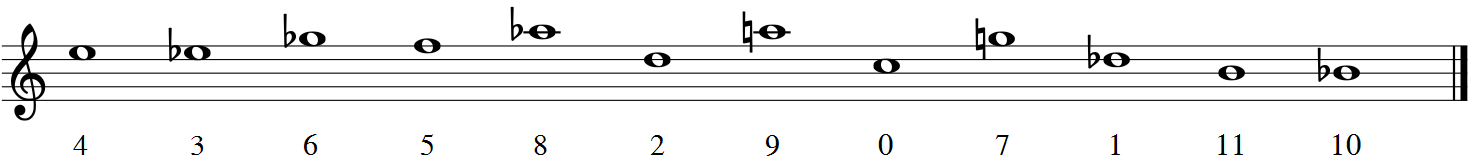
\includegraphics[width=\textwidth]{7.png}
	\bigskip\bigskip
	$$\text{IRT}^0=\left(\begin{matrix}0&1&2&3&4&5&6&7&8&9&10&11\\10&11&8&9&6&0&5&2&7&1&3&4\\\end{matrix}\right)$$
	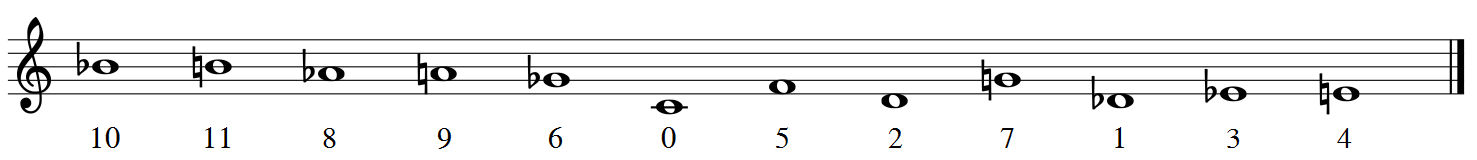
\includegraphics[width=\textwidth]{5.png}
	\bigskip\bigskip
	$$\text{IRT}^6=\left(\begin{matrix}0&1&2&3&4&5&6&7&8&9&10&11\\4&5&2&3&0&6&11&8&1&7&9&10\\\end{matrix}\right)$$
	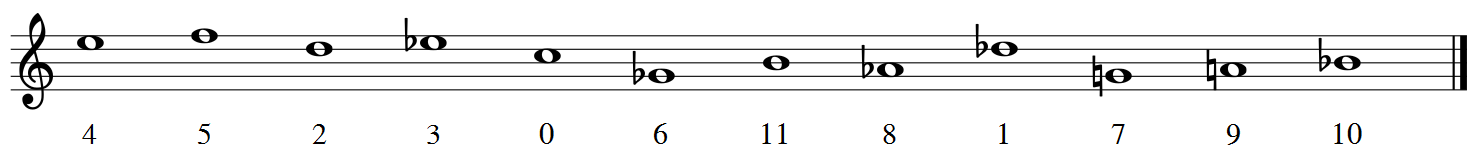
\includegraphics[width=\textwidth]{8.png}%
%    \chapter{Análisis serial de la Musette}
	\label{app:score}
    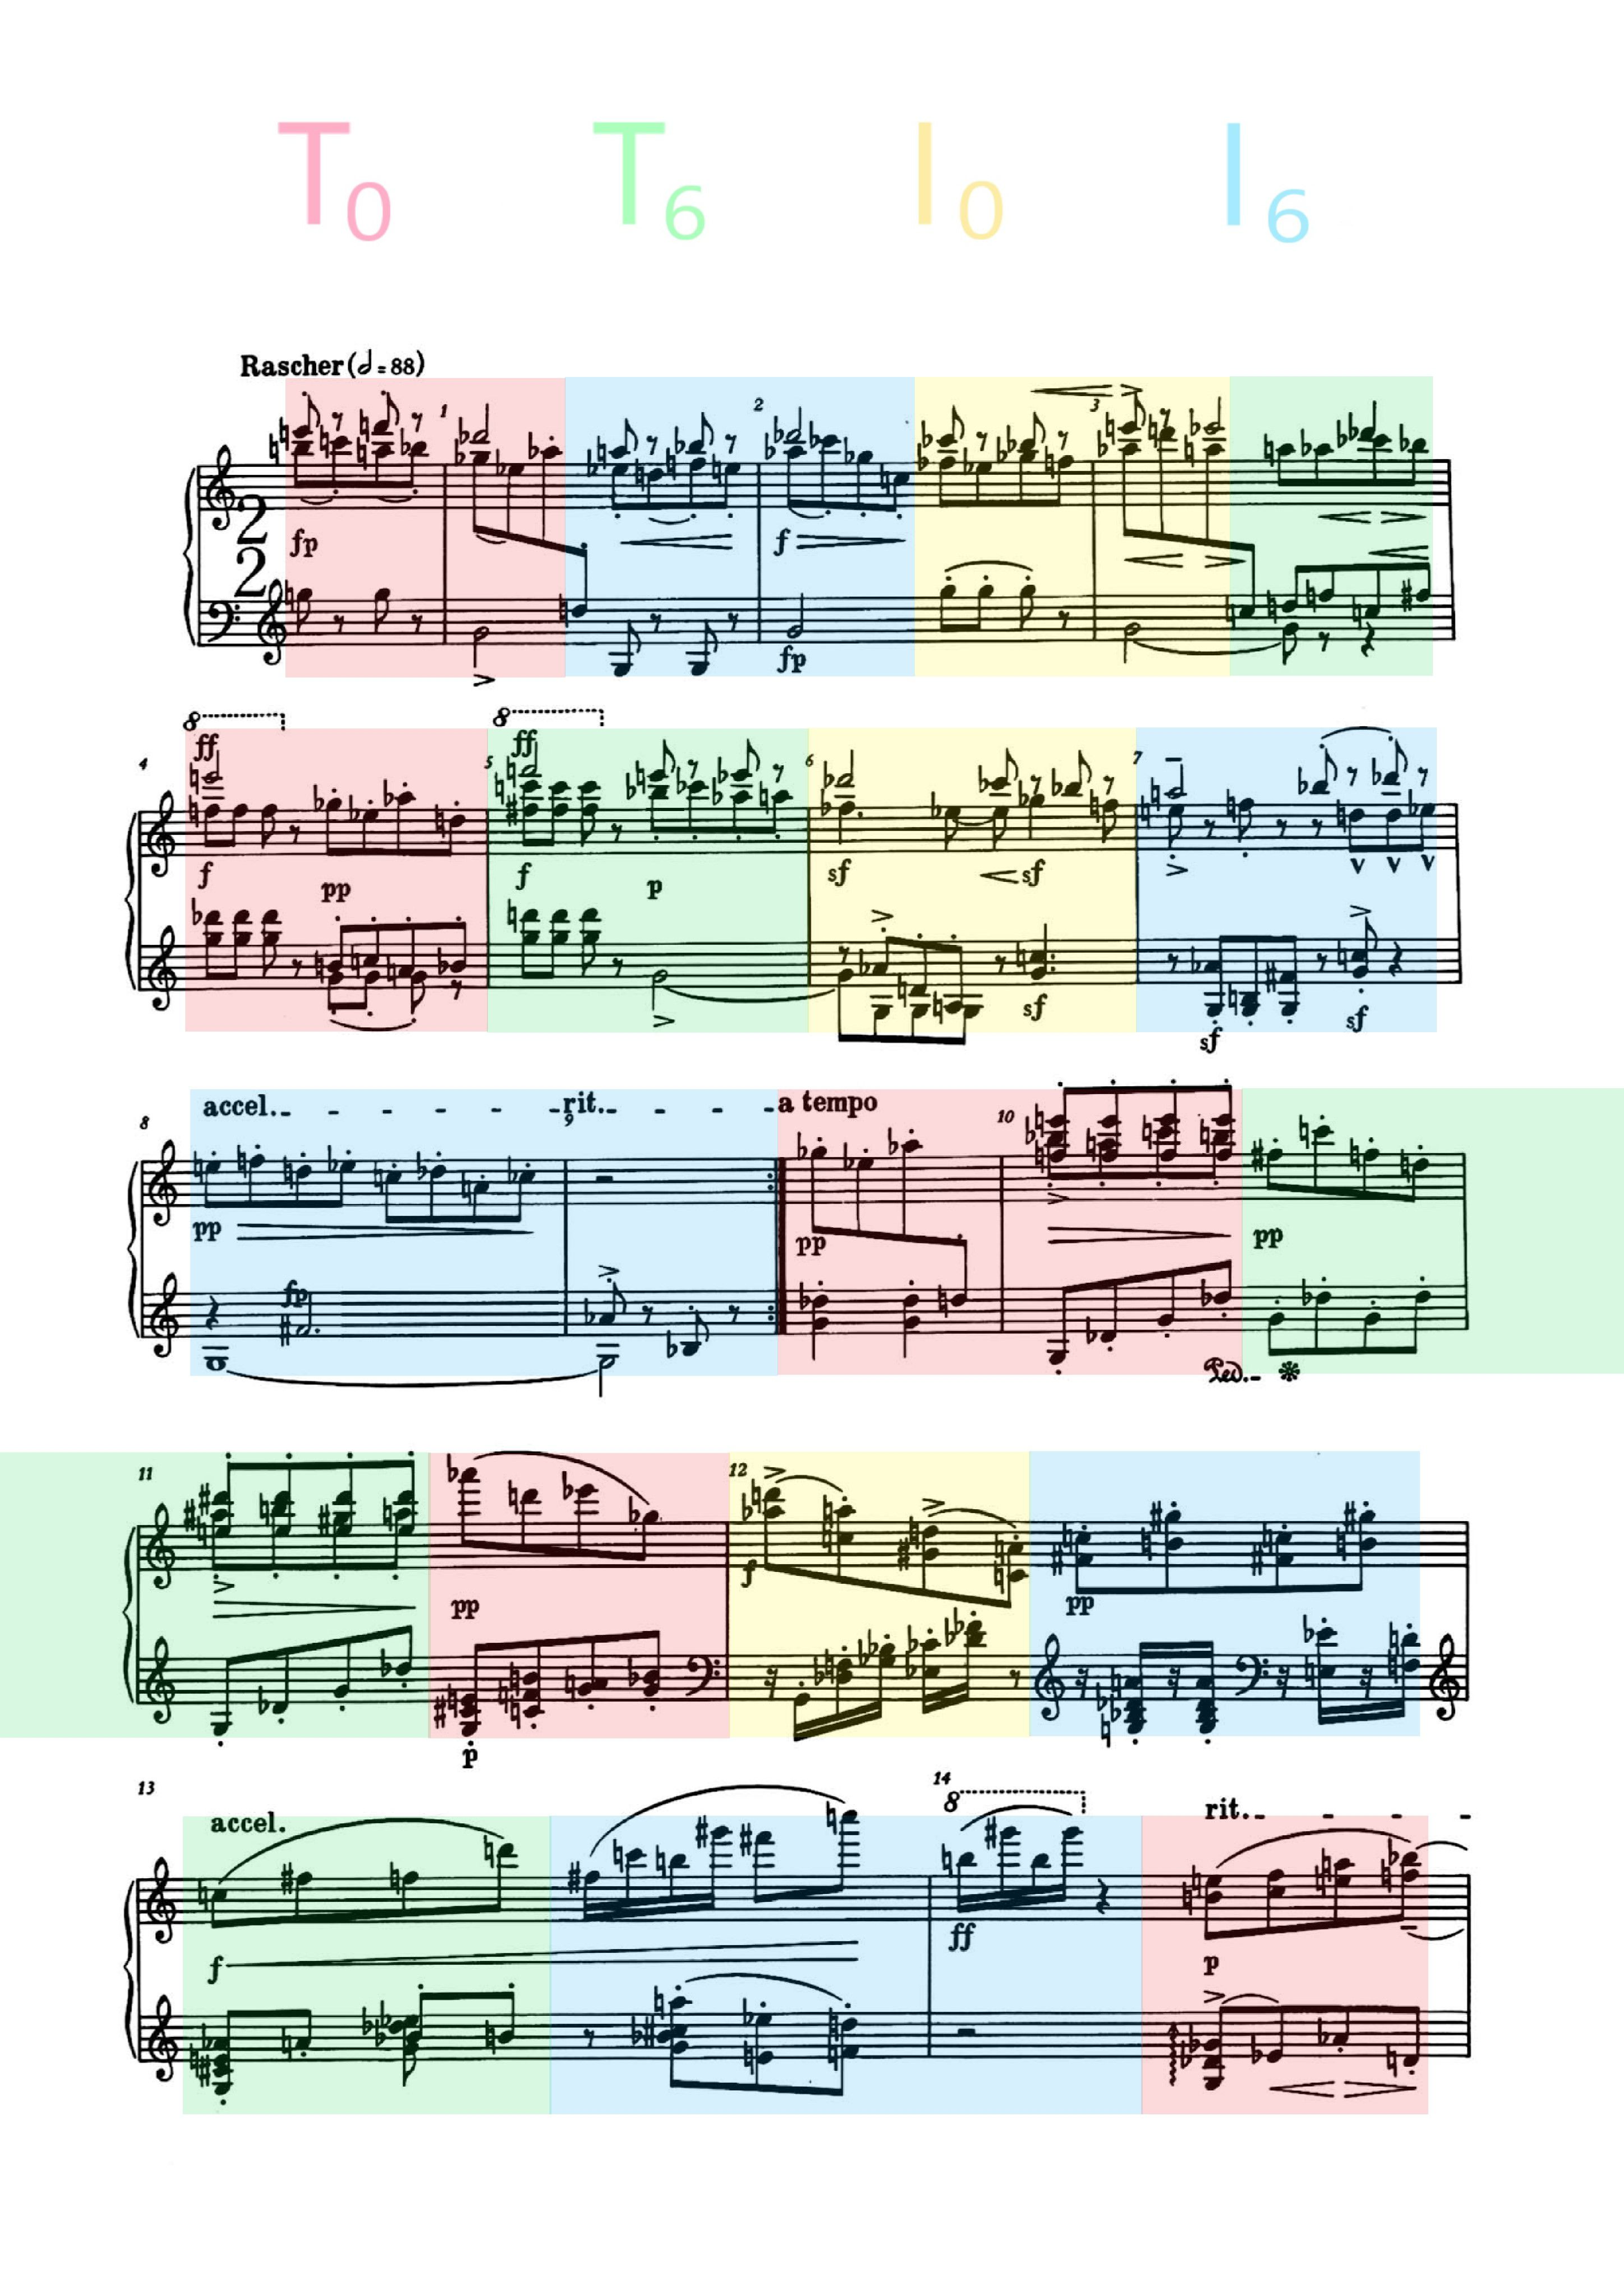
\includepdf[pages=-]{Anexos/Musette.pdf}%
    	\chapter[Conmutatividad del grupo D$_{\textbf{12}}$ x D$_{\textbf{12}}$]{Conmutatividad del grupo \\D$_{\textbf{12}}$ x D$_{\textbf{12}}$}
	\label{app:commm}
		\subsubsection*{S y T no conmutan:}
		
		$\text{S}\circ\text{T}(\sigma(m))=\text{S}(\sigma(m)+1)=-(\sigma(m)+1)=-\sigma(m)-1$
		
		$\text{T}\circ\text{S}(\sigma(m))=\text{T}(-\sigma(m))=-\sigma(m)+1$
		
		$\text{S}\circ\text{T}^{-1}(\sigma(m))=\text{S}(\sigma(m)-1)=-(\sigma(m)-1)=-\sigma(m)+1=\text{T}\circ\text{S}(\sigma(m))$
		
		\subsubsection*{V y C no conmutan:}
		
		$\text{V}\circ\text{C}(\sigma(m))=\text{V}(\sigma(m+1))=\sigma(-(m+1))=\sigma(-m-1)$
		
		$\text{C}\circ\text{V}(\sigma(m))=\text{C}(\sigma(-m))=\sigma(-m+1)$
		
		$\text{V}\circ\text{C}^{-1}(\sigma(m))=\text{V}(\sigma(m-1))=\sigma(-(m-1))=\sigma(-m+1)=\text{C}\circ\text{V}(\sigma(m))$
		
		\subsubsection*{S y V conmutan:}
		
		$\text{S}\circ\text{V}(\sigma(m))=\text{S}(\sigma(-m))=-\sigma(-m)$
		
		$\text{V}\circ\text{S}(\sigma(m))=\text{V}(-\sigma(m))=-\sigma(-m)$
		
		\subsubsection*{S y C conmutan:}
		
		$\text{S}\circ\text{C}(\sigma(m))=\text{S}(\sigma(m+1))=-\sigma(m+1)$
		
		$\text{C}\circ\text{S}(\sigma(m))=\text{C}(-\sigma(m))=-\sigma(m+1)$
		
		\subsubsection*{T y V conmutan:}
		
		$\text{T}\circ\text{V}(\sigma(m))=\text{T}(\sigma(-m))=\sigma(-m)+1$
		
		$\text{V}\circ\text{T}(\sigma(m))=\text{V}(\sigma(m)+1)=\sigma(-m)+1$
		
		\subsubsection*{T y C conmutan:}
		
		$\text{T}\circ\text{C}(\sigma(m))=\text{T}(\sigma(m+1))=\sigma(m+1)+1$
		
		$\text{C}\circ\text{T}(\sigma(m))=\text{C}(\sigma(m)+1)=\sigma(m+1)+1$
    	\chapter{Código para generar funciones E-inducidas}
	\label{app:function}
	
	\lstset{
		language=Haskell,
		identifierstyle=\color{black},
	}
	
	\newpage
	\lstinputlisting{Anexos/function.hs}
\end{appendices}
    
	\cleardoublepage
    
		\begin{thebibliography}{00}
		\addcontentsline{toc}{chapter}{Bibliografía}
			
%			\item Introducción:
			
			\bibitem{wright}
			{\sc Wright, David.} 
			\textit{Mathematics and Music},
			American Mathematical Society 
			(2009).
			
%			\item Historia:
			
%			\bibitem{kinney}
%			{\sc Kinney, James P.} 
%			\textit{Twelve-tone Serialism: Exploring the Works of Anton Webern},
%			Undergraduate Honors Theses.
%			Paper 1
%			(2015)
%			
%			\bibitem{diaz}
%			{\sc Díaz de la Fuente, Alicia.} 
%			\textit{Estructura y significado en la música serial y aleatoria},
%			Universidad Nacional de Educación a Distancia.
%			Tesis Doctoral en Filosofía
%			(2005)
%			
%			\bibitem{delgado}
%			{\sc Prof. Fernando Delgado García.} 
%			Clases y material de Historia de la Música, 5$^{\circ}$ y 6$^{\circ}$ de Enseñanzas Profesionales del Conservatorio Profesional de Música Arturo Soria, cursos 2014-15 y 2015-16.
			
%			NADA
%			\bibitem{dominguez}
%			{\sc Domínguez Romero, Manuel.} 
%			\textit{Las Matemáticas en el Serialismo Musical},
%			Sigma n.24 
%			(2004).

%			\item Suite:
					
%			\bibitem{xiao}
%			{\sc Xiao, June.} 
%			\textit{Bach’s Influences in the Piano Music of Four 20th Century Composers},
%			Indiana University Jacobs School of Music.
%			Doctoral Theses in Music
%			(2014)
%			
%			\bibitem{clercq}
%			{\sc Clercq, Trevor de.} 
%			\textit{A Window into Tonality via the Structure of Schoenberg's ``Musette'' from the Piano Suite, op. 25},
%			Theory/Analysis of 20th-Century Music.
%			Prof. David Headlam
%			(2006)
%			
%			\bibitem{hyde}
%			{\sc Hyde, Martha.} Chapter 4: “Dodecaphonism: Schoenberg”,
%			\textit{Models of Musical Analysis: Early Twentieth-century Music},
%			Ed. Mark Everist and Jonathan Dunsby.
%			Oxford: Blackwell
%			(1993)
%			
%			\bibitem{ilomaki}
%			{\sc Ilom\"aki, Tuukka.}
%			\textit{On the Similarity of Twelve-Tone Rows},
%			Sibelius Academy
%			(2008).
			
%			\item Acciones:
			
%			\bibitem{armstrong}
%			{\sc Armstrong, M. A.} Chapter 6: “Permutations”, Chapter 17: “Actions, Orbits, and Stabilizers”, Chapter 18: “Counting Orbits”,
%			\textit{Groups and Symmetry},
%			New York: Springer-Verlag
%			(1988)
			
%			\item Espectros:
			
			\bibitem{polygons}
			{\sc Golomb, S. W., Welch, L. R.}
			\textit{On the enumeration of polygons},
			The American Mathematical Monthly, Vol. 67, 349-353
			(1960).
			
			\bibitem{reiner}
			{\sc Reiner, David L.}
			\textit{Enumeration in Music Theory},
			The American Mathematical Monthly, Vol. 92, No. 1
			(1985).
			
%			\item Filosofía:
			
%			\bibitem{basomba}
%			{\sc Basomba García, Daniel.} 
%			\textit{El último Bach y el dodecafonismo como ideal musical: una lectura estética y sociológica},
%			Universidad Carlos III de Madrid.
%			Tesis Doctoral en Ciencia Política y Sociología
%			(2013)
			
%			NADA
%			\bibitem{bhalerao}
%			{\sc Bhalerao, Rasika.} 
%			\textit{The Twelve-Tone Method of Composition},
%			Math 336.
%			Prof. Jim Morrow
%			(2015)
			
%			NADA
%			\bibitem{morris}
%			{\sc Morris, Robert.}
%			\textit{Mathematics and the Twelve-Tone System: Past, Present, and Future},
%			Perspectives of New Music 45.2 
%			(2007)
			
%			NADA
%			\bibitem{cook}
%			{\sc Cook, Nicholas.} Chapter 9: “Analyzing Serial Music”,
%			\textit{A Guide to Musical Analysis},
%			New York: G. Braziller
%			(1987)
			
%			NADA
%			\bibitem{roberts}
%			{\sc Roberts, Gareth E.}
%			\textit{Composing with Numbers: Arnold Schoenberg and His Twelve-Tone Method},
%			Math/Music: Aesthetic Links
%			(2012).
			
%			NADA
%			\bibitem{hunter}
%			{\sc Hunter, David J.; von Hippela, Paul T.}
%			\textit{How Rare Is Symmetry in Musical 12-Tone Rows?},
%			The American Mathematical Monthly, Vol. 110, No. 2
%			(2003).
			
%			NADA
%			\bibitem{rowdata}
%			{\sc London, J., von Hippel, P., Huron, D., Cartano, J., Kingery, K., Olsen, B., Santelli, T.}
%			\textit{Row forms in the serial works of Schoenberg, Berg, and Webern}
%			[Computer database.] Stanford, CA: Center for Computer Assisted Research in the Humanities (www.ccarh.org/publications/data/humdrum/tonerow/) (2000/2001).
						
	\end{thebibliography}

	\cleardoublepage
    
\end{document}